\documentclass[SE,lsstdraft,authoryear,toc]{lsstdoc}
\input{meta}

% Package imports go here.
\usepackage{subcaption}                 % supports \begin{subfigure}...\end{subfigure}
\usepackage{xspace}

% Local commands go here.
\newcommand{\ComCam}{ComCam\xspace}
\setlength{\headheight}{62pt}           % heed warnings that these values need adjusting
\addtolength{\topmargin}{-7pt}

%If you want glossaries
%\input{aglossary.tex}
%\makeglossaries

\title{An Interim Report on the ComCam On-Sky Campaign}

% This can write metadata into the PDF.
% Update keywords and author information as necessary.
\hypersetup{
    pdftitle={An Interim Report on the ComCam On-Sky Campaign},
    pdfauthor={SITCOM G6},
    pdfkeywords={}
}

% Optional subtitle
% \setDocSubtitle{A subtitle}

\author{%
On behalf of Rubin Observatory Project
}

\setDocRef{SITCOMTN-149}
\setDocUpstreamLocation{\url{https://github.com/lsst-sitcom/sitcomtn-149}}

\date{\vcsDate}

% Optional: name of the document's curator
% \setDocCurator{The Curator of this Document}

\setDocAbstract{%
A summary of what we have learned from the initial period of ComCam observing
}

% Change history defined here.
% Order: oldest first.
% Fields: VERSION, DATE, DESCRIPTION, OWNER NAME.
% See LPM-51 for version number policy.
\setDocChangeRecord{%
  \addtohist{1}{YYYY-MM-DD}{Unreleased.}{Robert Lupton}
}


\begin{document}

% Create the title page.
\maketitle
% Frequently for a technote we do not want a title page  uncomment this to remove the title page and changelog.
% use \mkshorttitle to remove the extra pages

% ADD CONTENT HERE
% You can also use the \input command to include several content files.

\section{Introduction}
\label{sec:introduction}

The Vera C. Rubin Observatory on-sky commissioning campaign using the Commissioning Camera (ComCam) began on 24 October 2024 and ended on 11 December 2024.
This interim report provides a concise summary of our understanding of the integrated system performance based tests and analyses conducted during the ComCam on-sky campaign.
The emphasis is distilling and communicating what we have learned about the system.
The report is organized into sections to describe major activities during the campaign, as well as multiple aspects of the demonstrated system and science performance.

\begin{warning}[Preliminary Results]
All of the results presented here are to be understood as work in progress using engineering data and the
initial versions of the data processing pipelines.
It is expected at this stage, in the middle of on-sky commissioning, that much of the discussion will concern open questions, issues, and anomalies that are actively being worked by the team.
Additional documentation will be provided as our understanding of the demonstrated performance of the as-built system progresses.
\end{warning}

\subsection{Charge}

\begin{note}[Charge Development Historical Note]
    The initial version of the charge developed in November 2024 is provided below for reference.
\end{note}

We identify the following high-level goals for the interim report:

\begin{itemize}

    \item \textbf{Rehearse workflows for collaboratively developing documentation} to describe our current understanding of the integrated system performance, e.g., to support the development of planned Construction Papers and release documentation to support the Early Science Program \citedsp{RTN-011}.
    This report represents an opportunity to collectively exercise the practical aspects of developing documentation in compliance with the policies and guidelines for information sharing during commissioning \citedsp{sitcomtn-076}.

    \item \textbf{Synthesize the new knowledge} gained from the ComCam on-sky commissioning campaign to inform the optimization of activities between the conclusion of the ComCam campaign and the start of the on-sky campaign with the LSST Camera (LSSTCam).

    \item \textbf{Inform the Rubin Science Community} on the progress of the on-sky commissioning campaign using ComCam.

\end{itemize}

Other planned systems engineering activities will specifically address system-level verification (\citedsp{lse-29} and \citedsp{lse-30}) using tests and analysis from the ComCam campaign.
While the analyses in this report will likely overlap with the generation of verification artifacts for systems engineering, and system-level requirement specifications will serve as key performance benchmarks for interpreting the progress to date, formal acceptance testing is not an explicit goal of this report.

\textbf{The groups within the Rubin Observatory project working on each of the activities and performance analyses are charged with contributing to the relevant sections of the report.}
The anticipated level of detail for the sections ranges from a paragraph up to a page or two of text, depending on the current state of understanding, with \textbf{quantitative performance} expressed as summary statistics, tables, and/or figures.
The objective for this document is to \textbf{summarize the state of knowledge of the system}, rather than how we got there or ``lessons learned''.
The sections refer to additional supporting documentation, e.g., analysis notebooks, other technotes with further detail, as needed.
Given the timelines for commissioning various aspects of the system, it is natural that some sections will have more detail than others.

The anticipated milestones for developing this interim report are as follows:

\begin{itemize}

    \item 18 Nov 2024: Define charge

    \item 4 Dec 2024: First drafts of report sections made available for internal review

    \item 18 Dec 2024: Revised drafts of report sections made available for internal review; editing for consistency and coherency throughout the report

    \item 14 Jan 2025: Initial version of report is released

    \item Mid-March 2025: Updated version of report is released based on further iterations of data processing and analysis (planned)

\end{itemize}

\begin{warning}[On-sky Pixel Image Embargo]
    All pixel images and representations of pixel images of any size field of view, including individual visit images, coadd images, and difference images based on ComCam commissioning on-sky observations must be kept internal to the Rubin Observatory Project team, and in particular, cannot be included in this report.
    Embargoed pixel images can only be referenced as authenticated links; unfortunately this means that
    there will be some links which cannot be followed by readers who are not members of the
    Rubin commissioning team.
    See \citedsp{sitcomtn-076} for details.
\end{warning}

\section{System Performance Analysis}
\label{sec:system_performance_analysis}

\newcommand{\TMAMotionSettings}{\href{https://rubinobs.atlassian.net/wiki/spaces/LSSTCOM/pages/53741249/TMA+Motion+Settings}{TMA Motion Settings}\xspace}
\newcommand{\testCase}[1]{\href{https://rubinobs.atlassian.net/projects/BLOCK?selectedItem=com.atlassian.plugins.atlassian-connect-plugin:com.kanoah.test-manager__main-project-page\#!/v2/testCase/#1}{#1}}

Topics to convert into text

\begin{itemize}
    \item M1M3 and M2 glass installed on the Simonyi Survey Telescope.
    \item Since then, we have been operating the telescope with limited velocity,
    acceleration, and jerk limits following the performances defined in \TMAMotionSettings.
    \item For each configuration, defined in terms of a percentage of the maximum
    velocity, acceleration, and jerk, we ran multiple gateway tests.
    \item The gateway tests are described in the \secRef{gateway_tests} below.
\end{itemize}

\subsection{Gateway Tests}
\label{sec:gateway_tests}

We started the ComCam on Sky test campaign using Simonyi Telescope with limited
performance, described as a percentage of the maximum velocity, acceleration,
and jerk limits. The performance is defined in \TMAMotionSettings Confluence page.

Before we can increase the telescope performance, we need to perform a set of
tests that ensure that the system will respond safely to the new velocity, acceleration,
and jerk. These tests are called gateway tests. Here is the list of all the tests.

\begin{itemize}
    \item \testCase{BLOCK-T227} Dynamic Tests at El = 34º short and long slews
    \item \testCase{BLOCK-T294} Dynamic Tests at El = 70º short and long slews
    \item \testCase{BLOCK-T231} TMA Azimuth Brake Test
    \item \testCase{BLOCK-T240} TMA Elevation Brake Distance
    \item \testCase{BLOCK-T241} M2 closed-loop break-out brake test during TMA slew
\end{itemize}


\subsubsection{Long and short slews at different elevations}
\label{subsubsec:long_and_short_slews}

These tests ensure that the force balance systems on M1M3 and on M2 can protect
the mirrors on different telescope positions and while slewing. As we increase
velocity, acceleration, and jerk limits, both mirrors suffer higher inertial
forces and the force actuators must counteract them.

%% TODO @b1quint - Ask Pablo, Holger, and Gabriele about the criteria for the
%% force balance systems for M2.
% For M1M3, the criteria is to keep the measured forces on the hardpoint actuators
% below the operational limit (15\% the breakaway limit). For M2, the criteria is
% ??????? (check with Holger, Gabriele, and Pablo).

The last set of data was collected on 2024-11-28. \figRef{block227_293_azel_slews}
shows the
slews performed when collecting this data starting at higher elevations (70$^\circ$)
and then moving to lower elevations (34$^\circ$).

\begin{center}
  \begin{figure}
    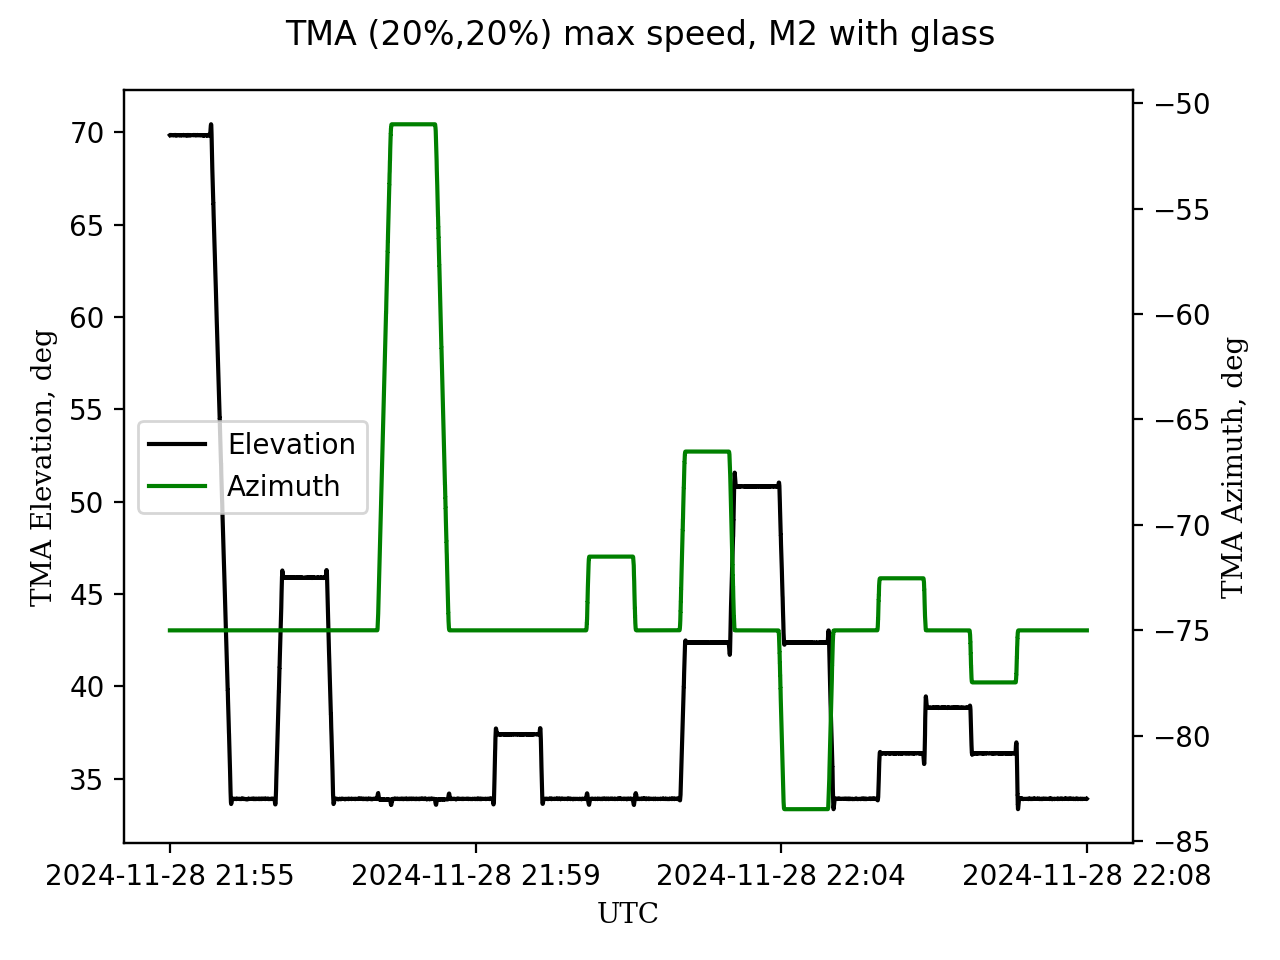
\includegraphics[width=0.5\textwidth]{spa/20_vel_acc_jerk/BLOCK-T227_azel_slews.png}
    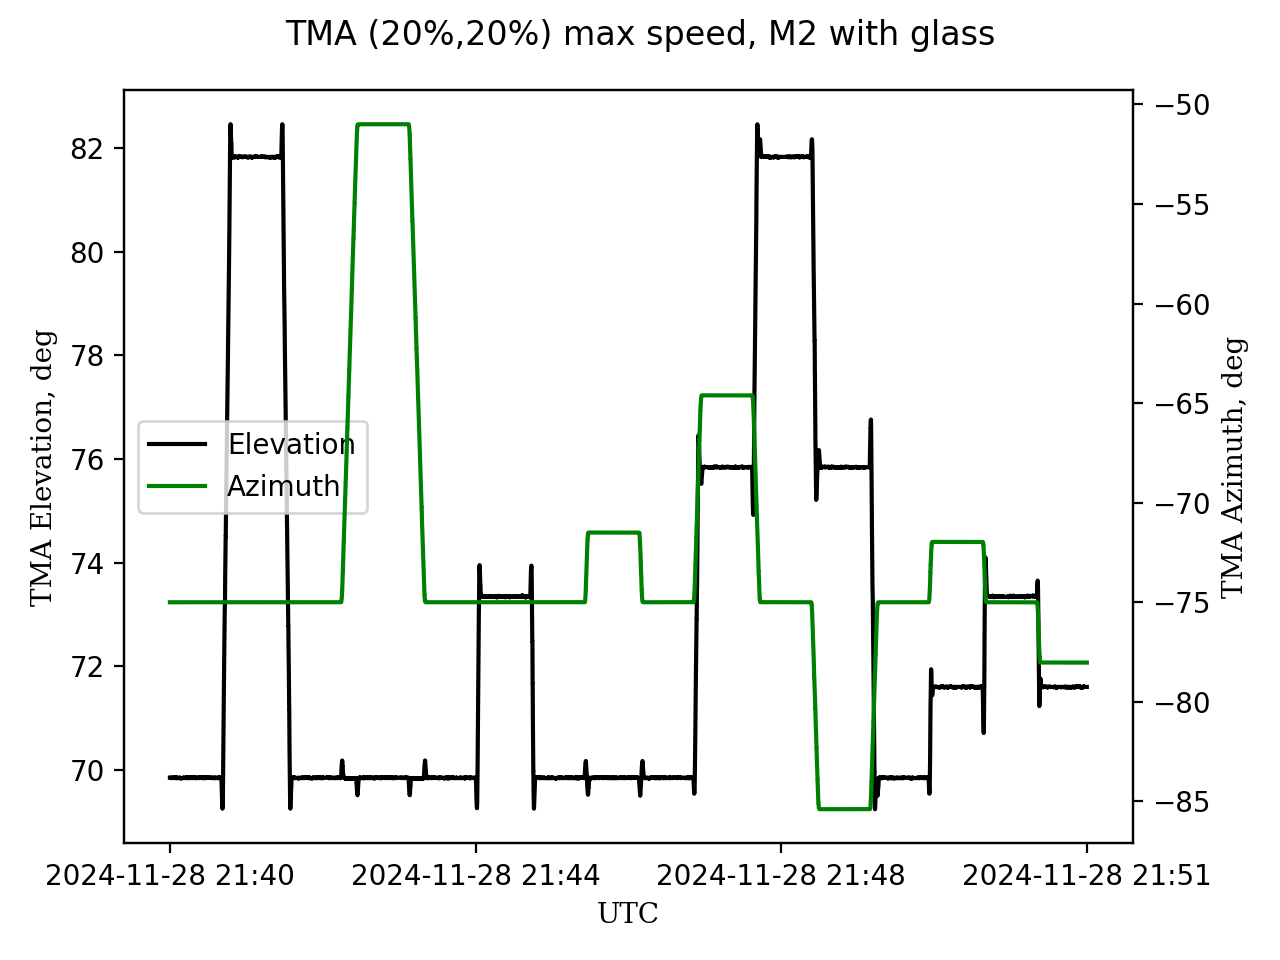
\includegraphics[width=0.5\textwidth]{spa/20_vel_acc_jerk/BLOCK-T293_azel_slews.png}
    \caption{TMA Short and Long slews at El = 34$^\circ$ (left) and El = 70$^\circ$ (right).}
    \label{fig:block227_293_azel_slews}
  \end{figure}
\end{center}

For each of these slews, the force balance system on M1M3 should keep the forces
measured on the hardpoints below an operational limit (15\% of the breakaway limit, nominally 450 N).
\figRefII{block227_m1m3_hp_histograms}{block293_m1m3_hp_histograms}
show histograms with the number of slews that hit certain minima
and maxima values for the hardpoint forces. The left histogram shows the minima
reached on each slew. The right histogram shows the maxima reached on each slew.
The red dashed lines show the fatigue limit (30\% of the breakaway limit, nominally 900 N).

You can see a few slews with min/max reaching 800 N at low elevations.
This is quite close to fatigue limits (900 N).
However, these slews were performed without booster valves enabled.
In addition, the big majority of the slews have measured forces below the operational limit.
This gave us confidence that, from M1M3's perpective, we can use the 20\% velocity, acceleration, and jerk for the rest of the campaign.
Note that we ran a few test slews with booster valves enabled and loads were significantly reduced (<200N per HP) before we got faults in some of the actuators with bad valves (need data analysis).

\begin{figure}
    \centering
    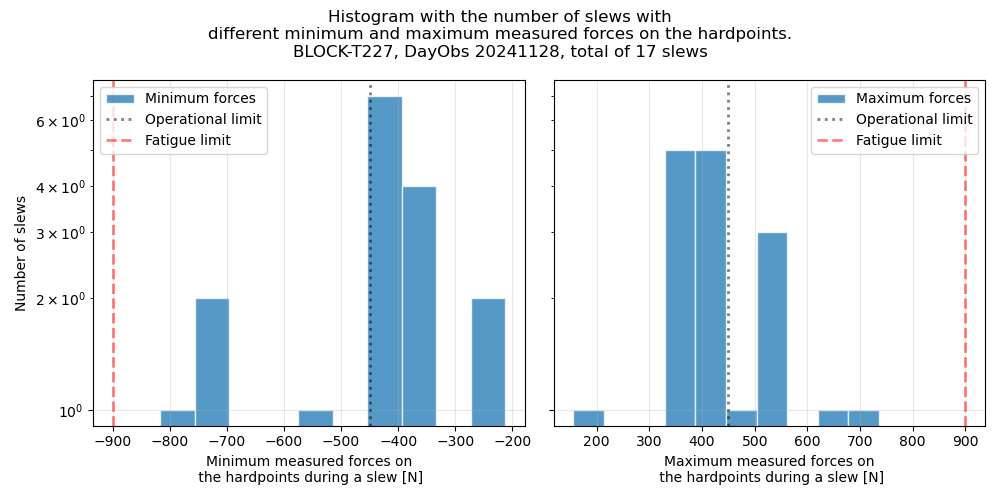
\includegraphics[width=0.8\textwidth]{spa/20_vel_acc_jerk/BLOCK-T227_m1m3_hp_histograms.png}
    \caption{M1M3 hardpoint histograms min/max HP forces at low elevation.}
    \label{fig:block227_m1m3_hp_histograms}
    \end{figure}

\begin{figure}
    \centering
    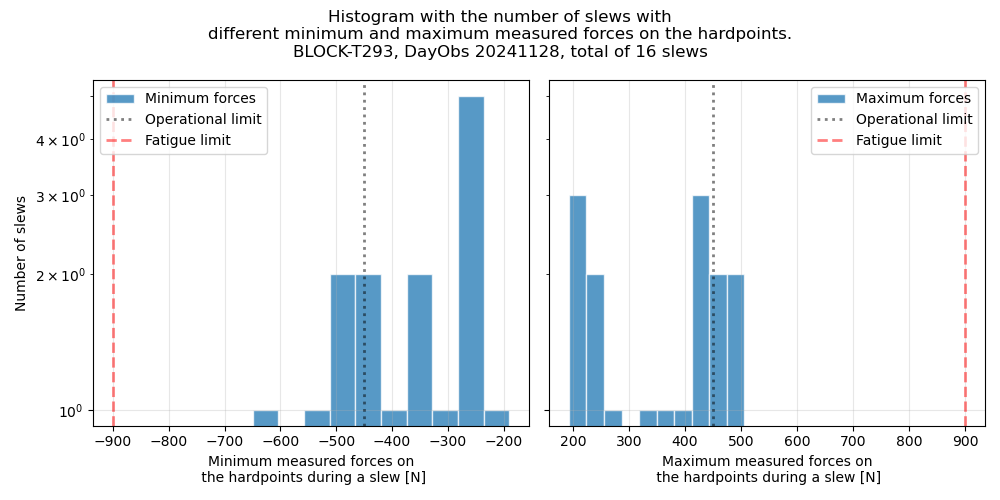
\includegraphics[width=0.8\textwidth]{spa/20_vel_acc_jerk/BLOCK-T293_m1m3_hp_histograms.png}
    \caption{M1M3 hardpoint histograms min/max HP forces at high elevation.}
    \label{fig:block293_m1m3_hp_histograms}
    \end{figure}

Similarly, M2 has limits of the measured forces associated with its closed loop and its
open loop.
\figRefIII{m2_axial_measured_forces}{m2_tangent_measured_forces}{m2_tangent_force_errors}
show the axial forces, the tangent forces, and the tangent
force errors for the slews performed at different elevations. We can see that, for every slew,
all the forces are within the closed loop maximum forces limit. This means that, from M2's
perpective, we are safe to operate the telescope with 20\% velocity, acceleration, and jerk.

\begin{figure}
    \centering
    \begin{subfigure}[b]{0.45\textwidth}
        \centering
        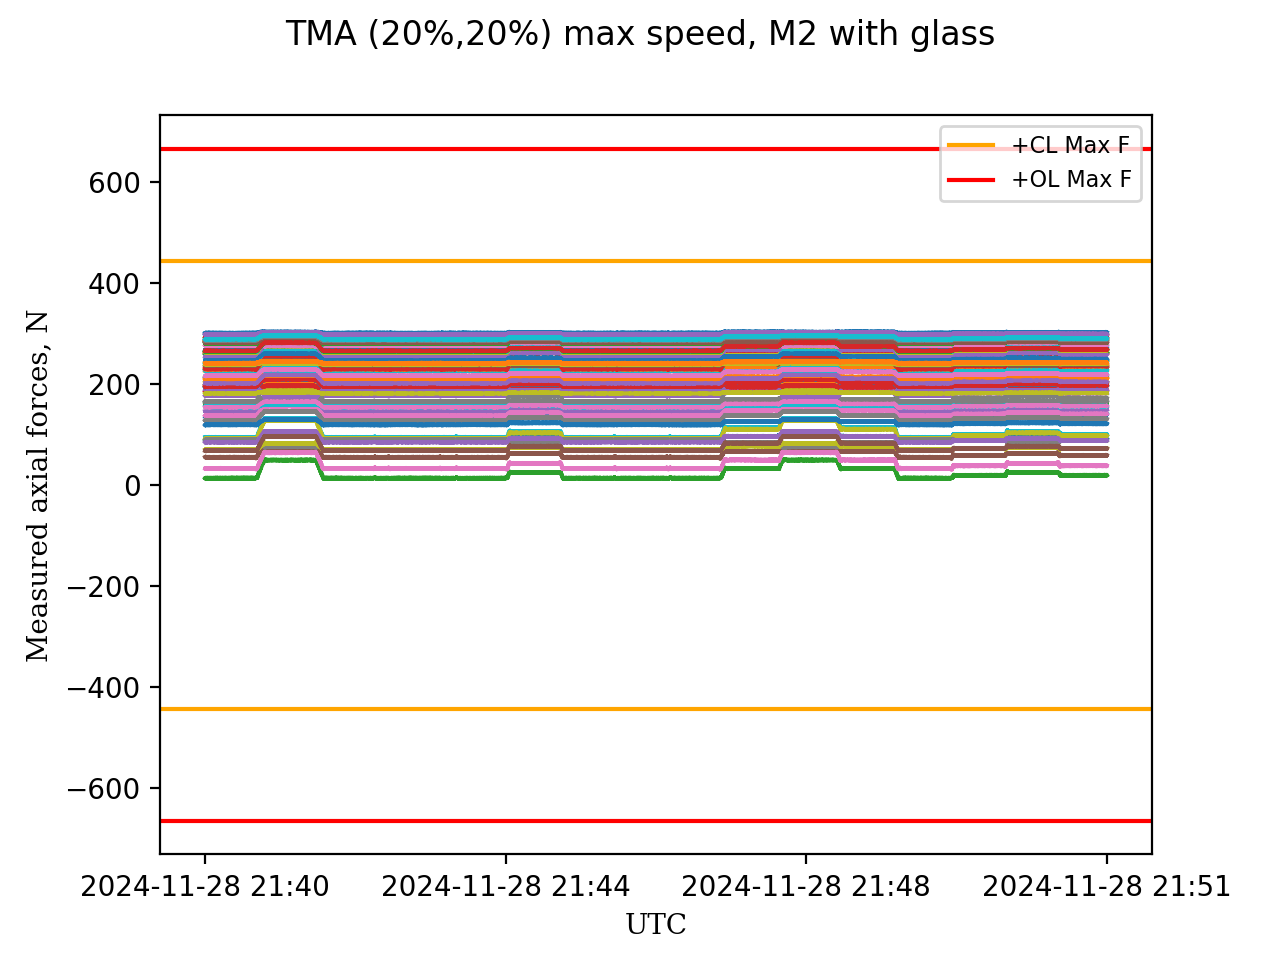
\includegraphics[width=\textwidth]{spa/20_vel_acc_jerk/BLOCK-T227_m2_axial_measured_forces.png}
        \caption{M2 axial measured forces at low elevation.}
        \label{fig:block227_m2_axial_measured_forces}
    \end{subfigure}
    \hfill
    \begin{subfigure}[b]{0.45\textwidth}
        \centering
        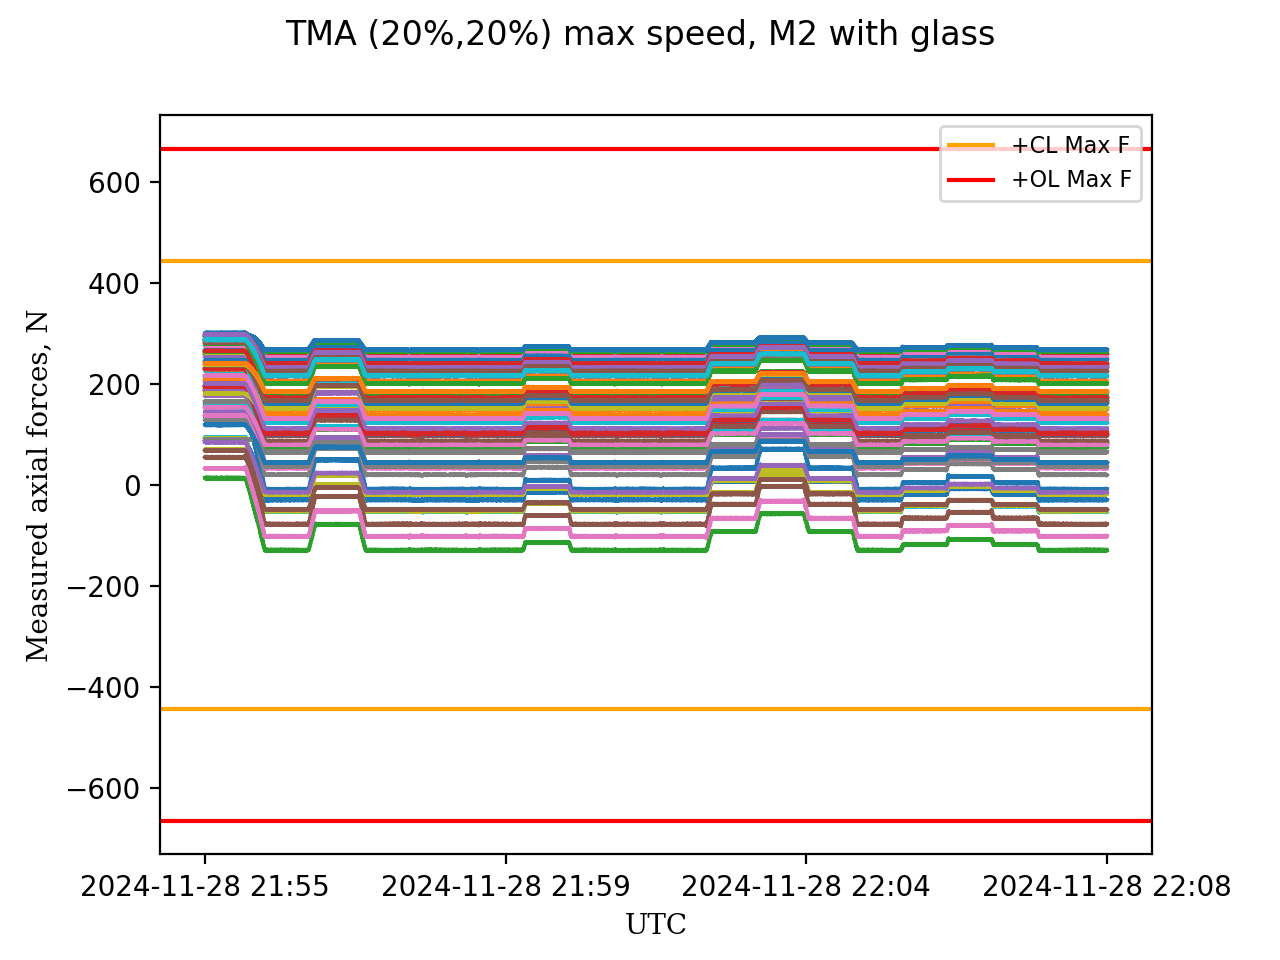
\includegraphics[width=\textwidth]{spa/20_vel_acc_jerk/BLOCK-T293_m2_axial_measured_forces.png}
        \caption{M2 axial measured forces at high elevation.}
        \label{fig:block293_m2_axial_measured_forces}
    \end{subfigure}
    \caption{M2 axial measured forces during the slews at different elevations.}
    \label{fig:m2_axial_measured_forces}
\end{figure}

\begin{figure}
    \centering
    \begin{subfigure}[b]{0.45\textwidth}
        \centering
        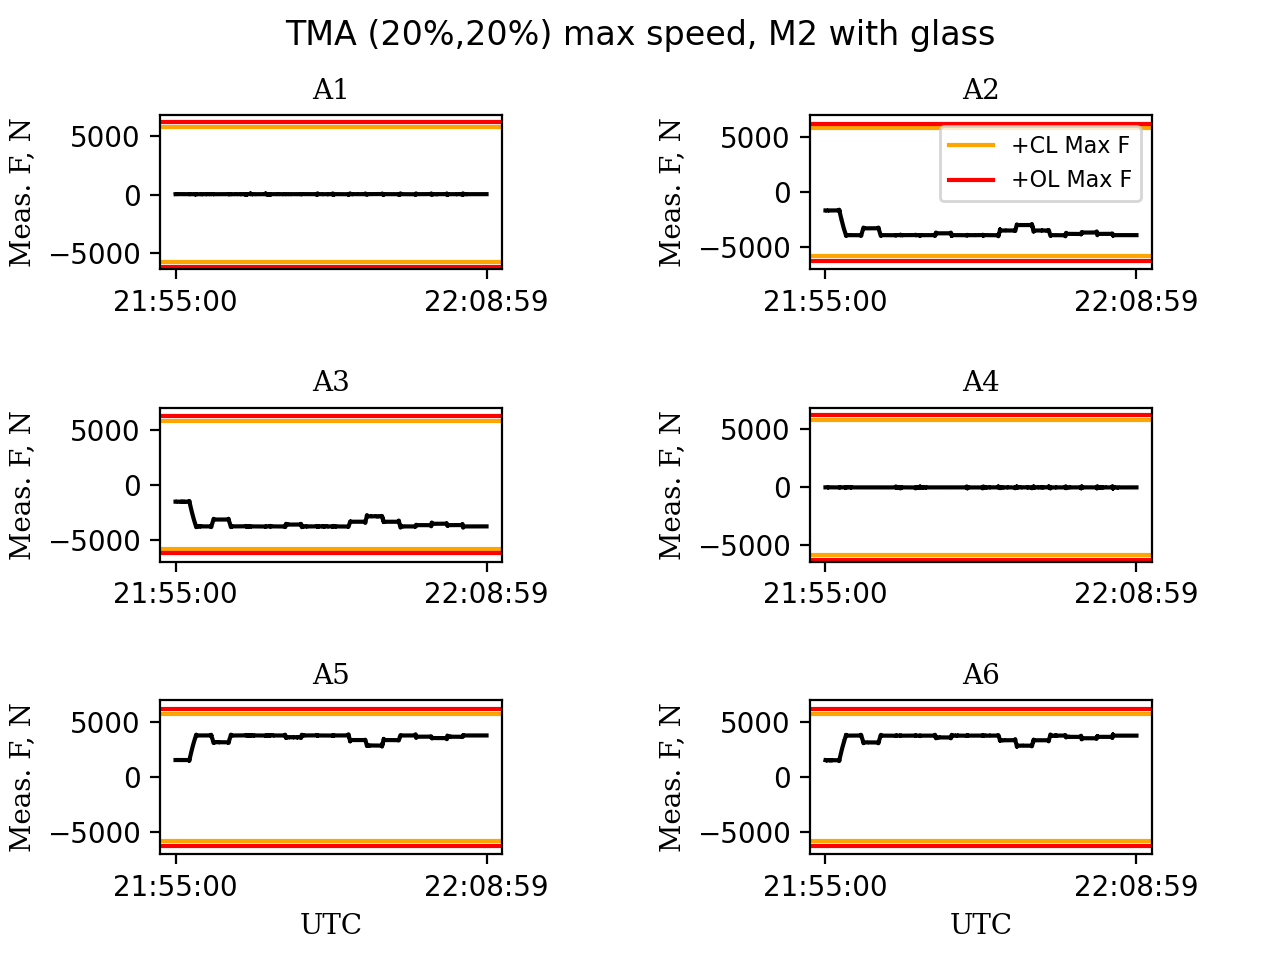
\includegraphics[width=\textwidth]{spa/20_vel_acc_jerk/BLOCK-T227_m2_tangent_measured_forces.png}
        \caption{M2 tangent force errors at low elevation.}
        \label{fig:block227_m2_tangent_measured_forces}
    \end{subfigure}
    \hfill
    \begin{subfigure}[b]{0.45\textwidth}
        \centering
        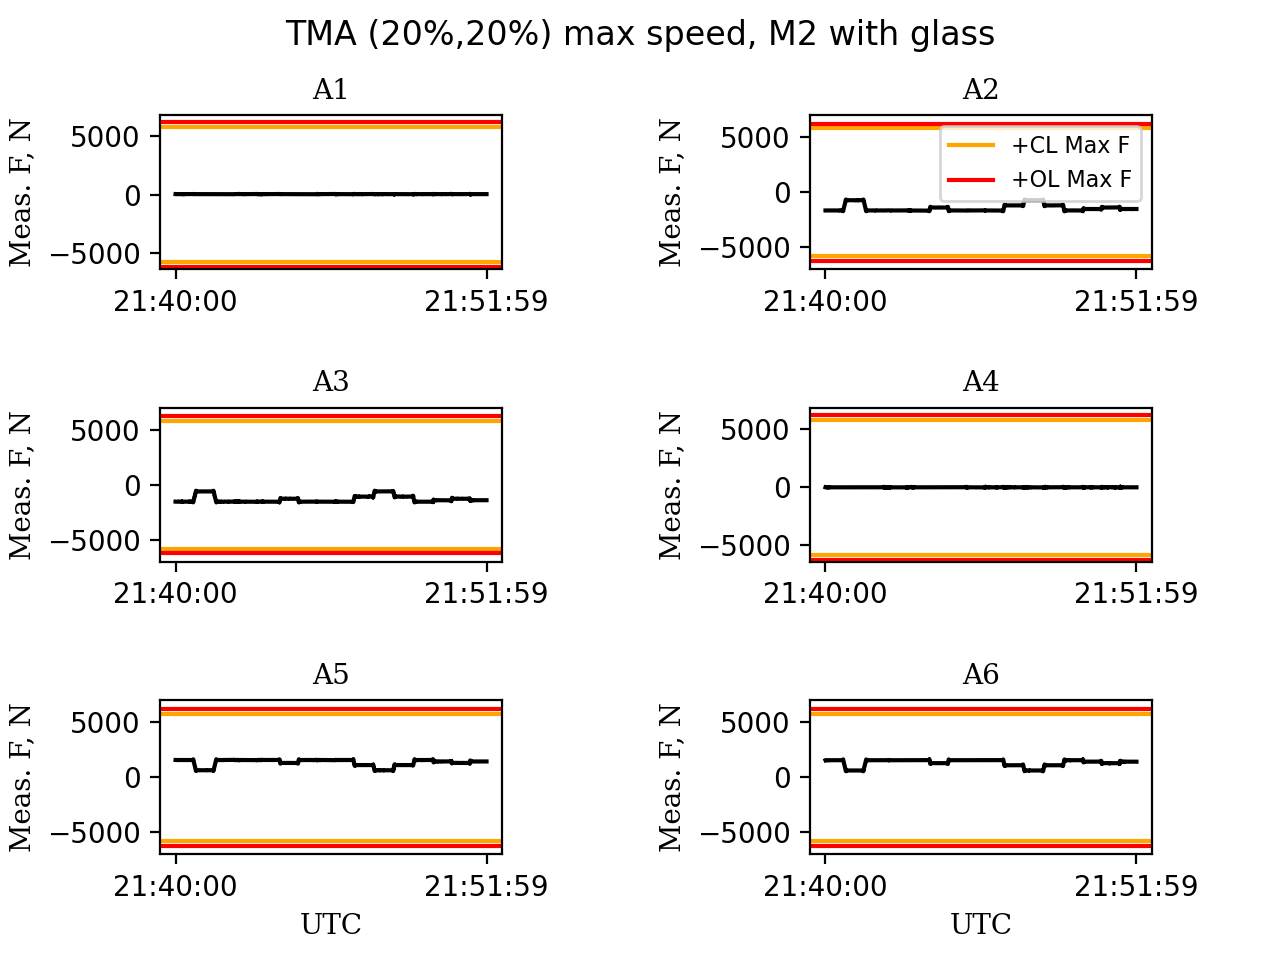
\includegraphics[width=\textwidth]{spa/20_vel_acc_jerk/BLOCK-T293_m2_tangent_measured_forces.png}
        \caption{M2 tangent force errors at high elevation.}
        \label{fig:block293_m2_tangent_measured_forces}
    \end{subfigure}
    \caption{M2 measured tangent forces during the slews at different elevations.}
    \label{fig:m2_tangent_measured_forces}
\end{figure}

\begin{figure}
    \centering
    \begin{subfigure}[b]{0.45\textwidth}
        \centering
        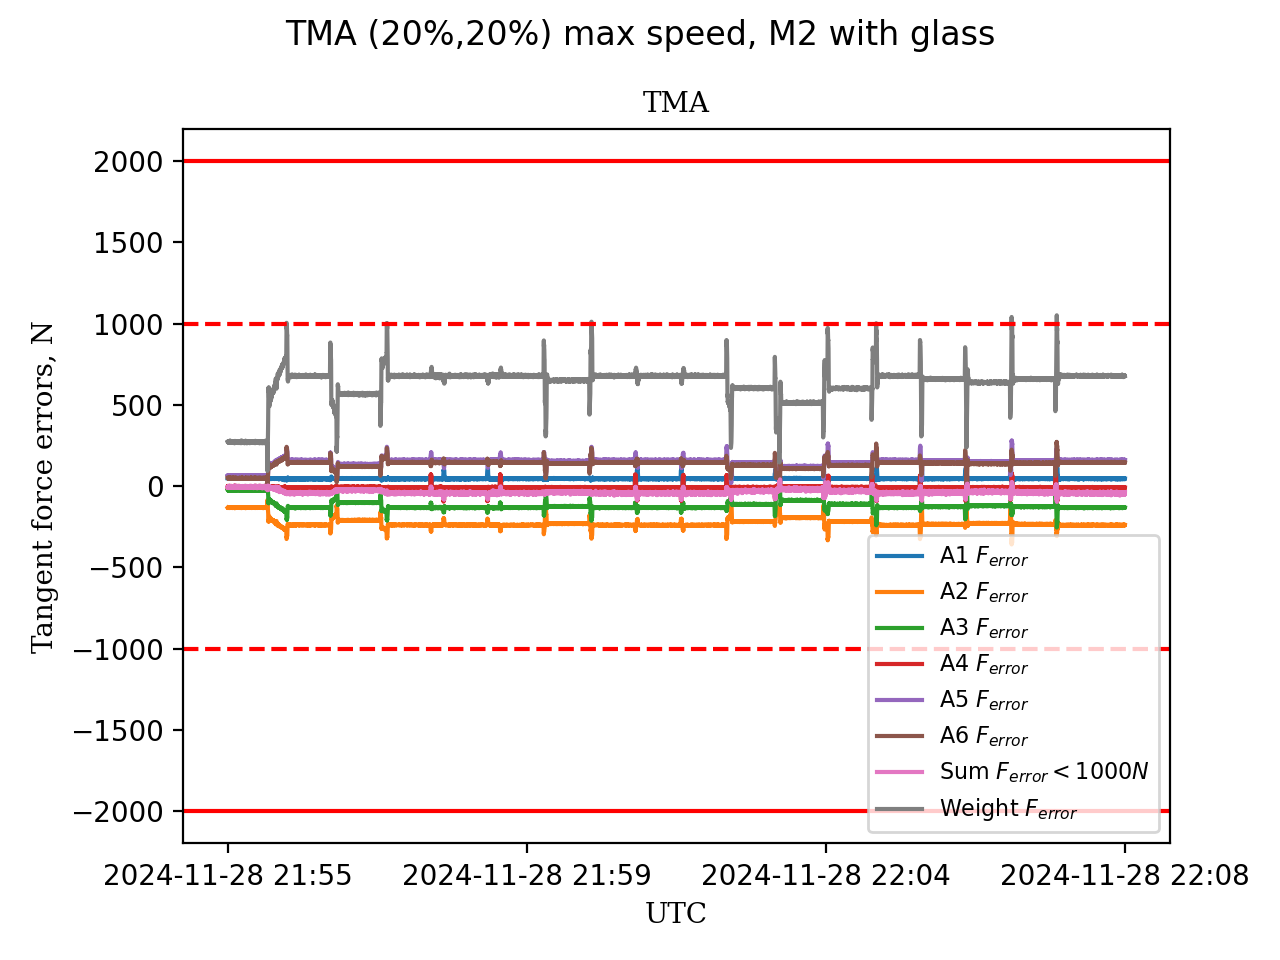
\includegraphics[width=\textwidth]{spa/20_vel_acc_jerk/BLOCK-T227_m2_tangent_force_errors.png}
        \caption{M2 tangent force errors at low elevation.}
        \label{fig:block227_m2_tangent_force_errors}
    \end{subfigure}
    \hfill
    \begin{subfigure}[b]{0.45\textwidth}
        \centering
        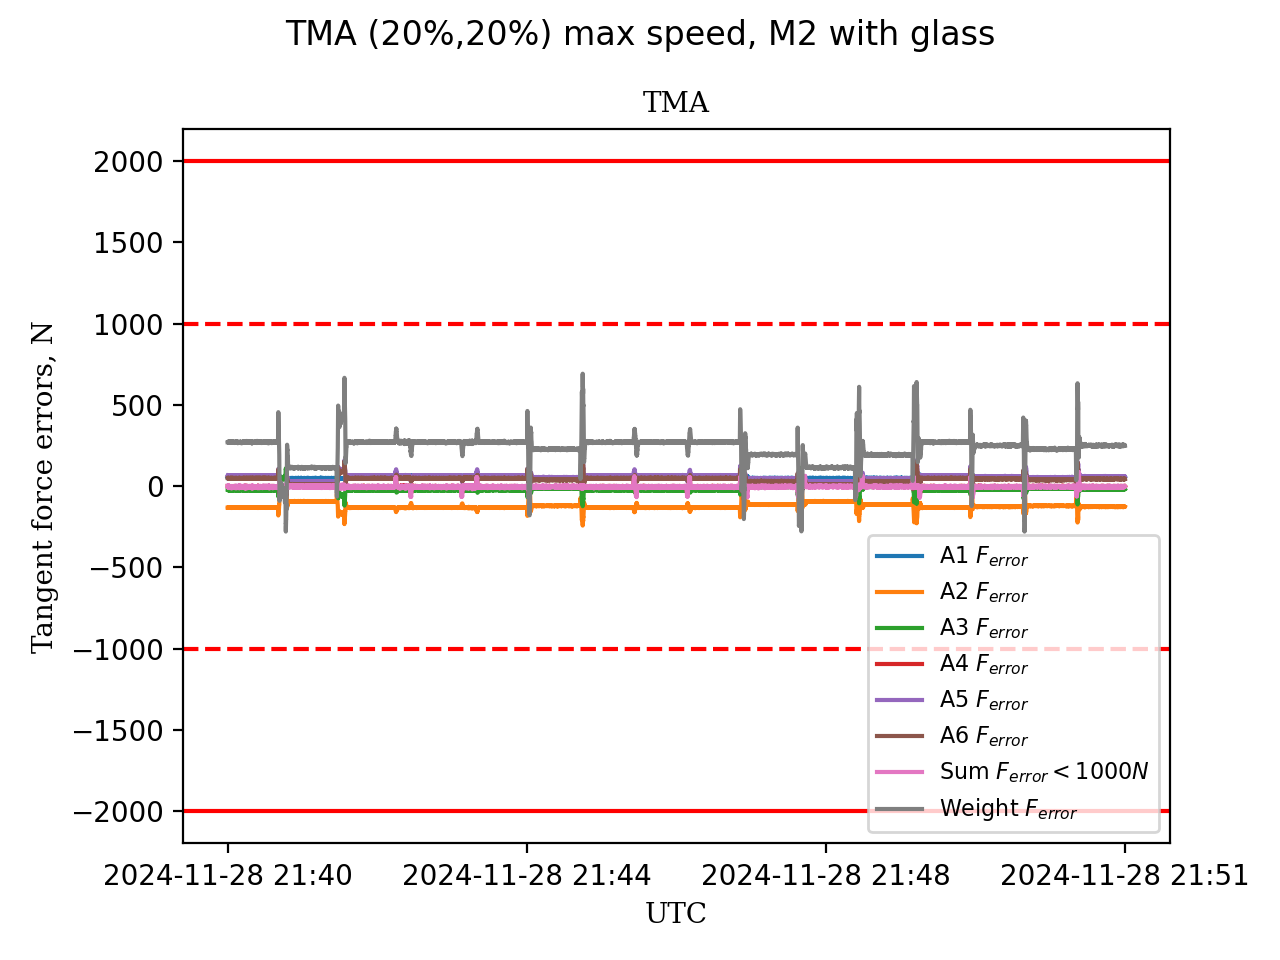
\includegraphics[width=\textwidth]{spa/20_vel_acc_jerk/BLOCK-T293_m2_tangent_force_errors.png}
        \caption{M2 tangent force errors at high elevation.}
        \label{fig:block293_m2_tangent_force_errors}
    \end{subfigure}
    \caption{M2 tangent force errors during the slews at different elevations.}
    \label{fig:m2_tangent_force_errors}
\end{figure}


\subsubsection{M2 close-loop breakout tests}
\label{subsubsec:m2_close_loop_breakout_tests}

\testCase{BLOCK-T241} M2 closed-loop break-out brake test during TMA slew is a test that
ensures that M2 can survive an event where the telescope is slewing and, for whatever reason,
the closed-loop system is disabled. In this case, the telescope will go to a fault and stop.

\figRefIII{block241_m2_axial_measured_forces}{block241_m2_tangent_measured_forces}{block241_m2_tangent_force_errors}
show the axial forces, the tangential forces, and the tangential force errors
during an event where the closed-loop system is disabled. The plots show that both axial and
tangential forces are within the limits. Considering this tests, we can say that M2 is safe to
operate with 20\% velocity, acceleration, and jerk.

\begin{figure}
    \centering
    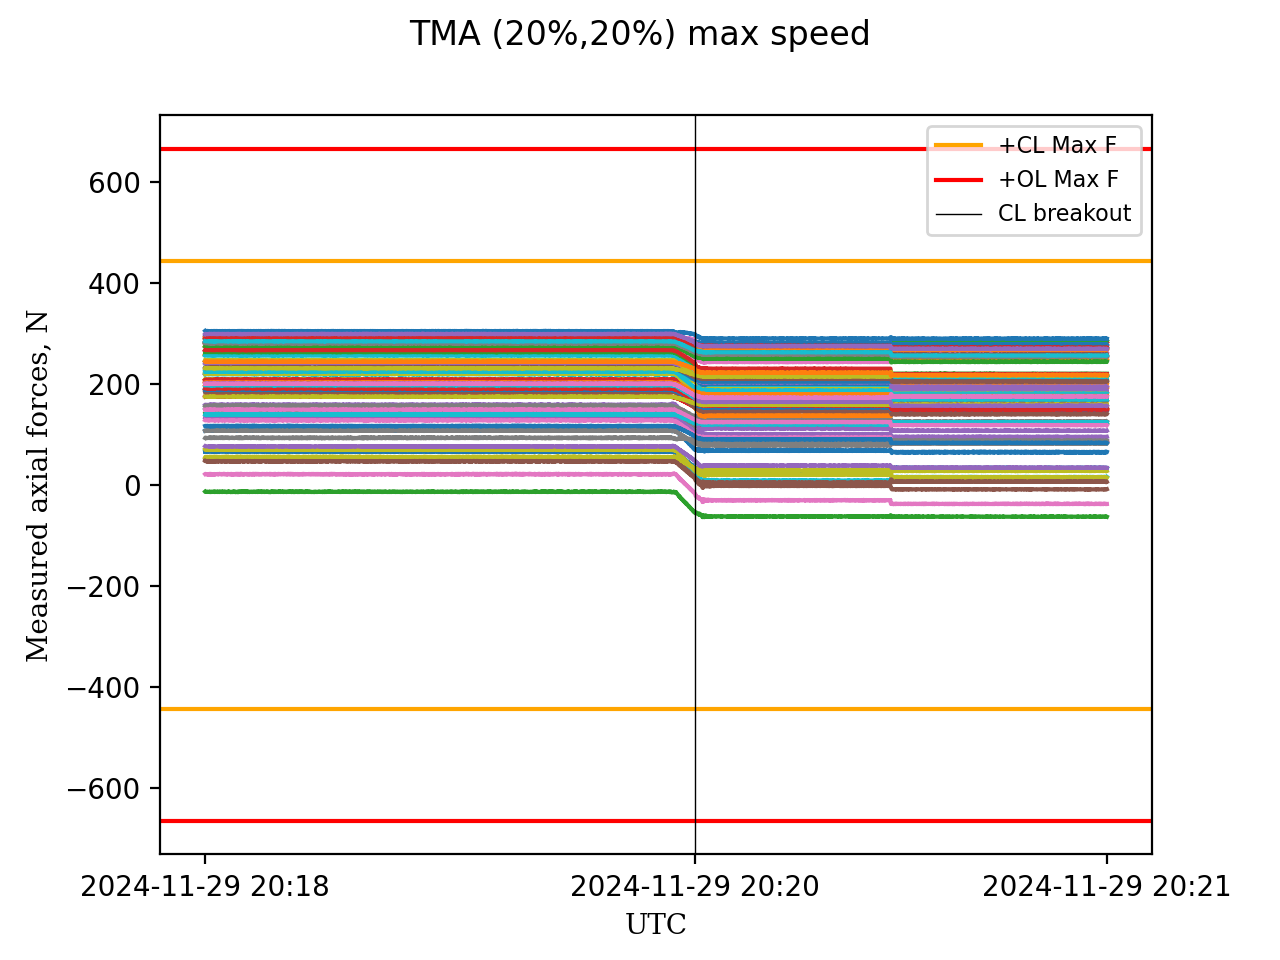
\includegraphics[width=0.8\textwidth]{spa/20_vel_acc_jerk/BLOCK-T241_m2_axial_measured_forces.png}
    \caption{M2 axial measured forces during the closed-loop break-out test.}
    \label{fig:block241_m2_axial_measured_forces}
    \end{figure}

\begin{figure}
    \centering
    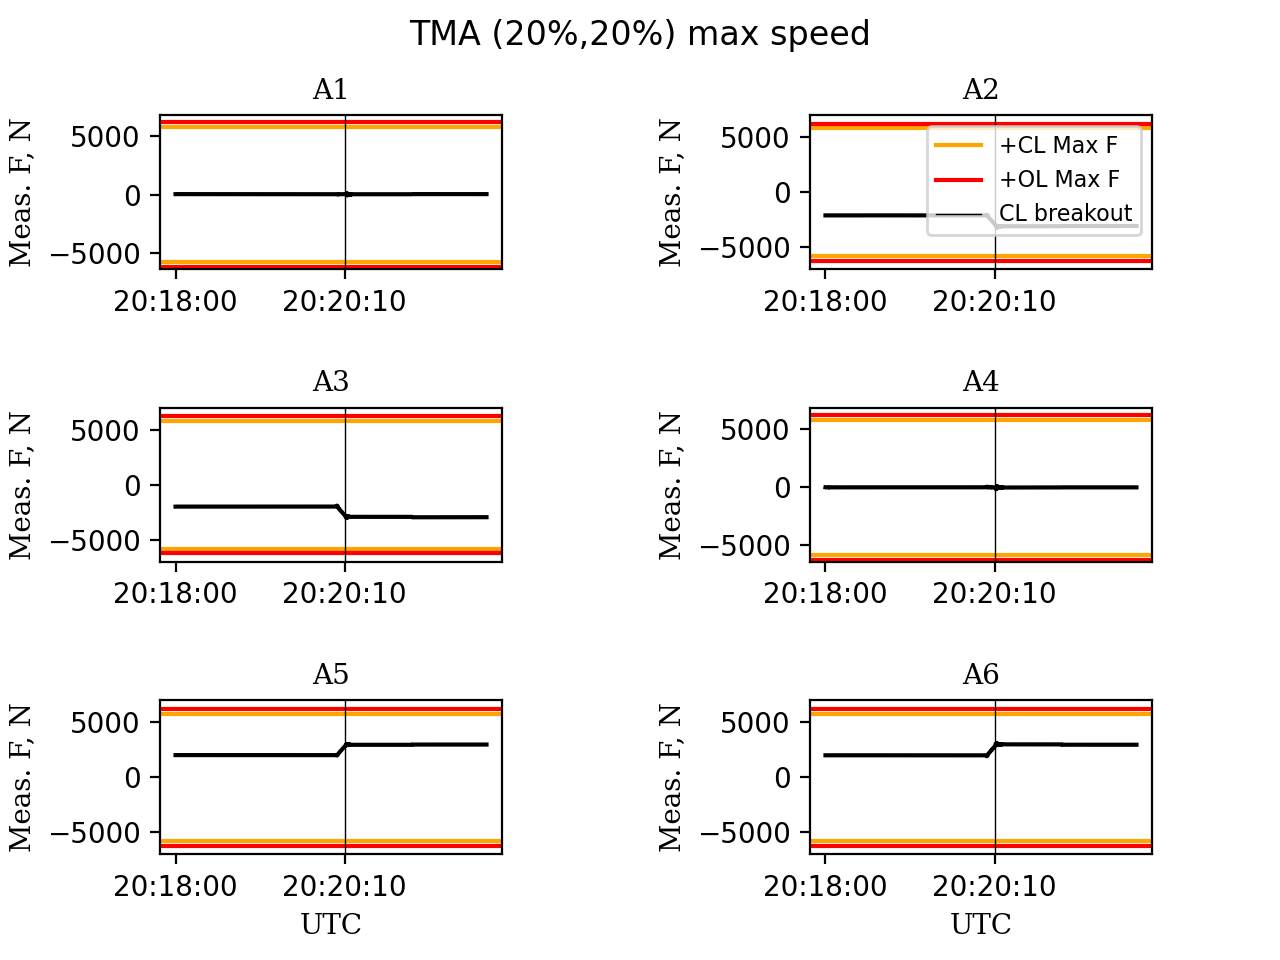
\includegraphics[width=0.8\textwidth]{spa/20_vel_acc_jerk/BLOCK-T241_m2_tangent_measured_forces.png}
    \caption{M2 tangential measured forces during the closed-loop break-out test.}
    \label{fig:block241_m2_tangent_measured_forces}
    \end{figure}

\begin{figure}
    \centering
    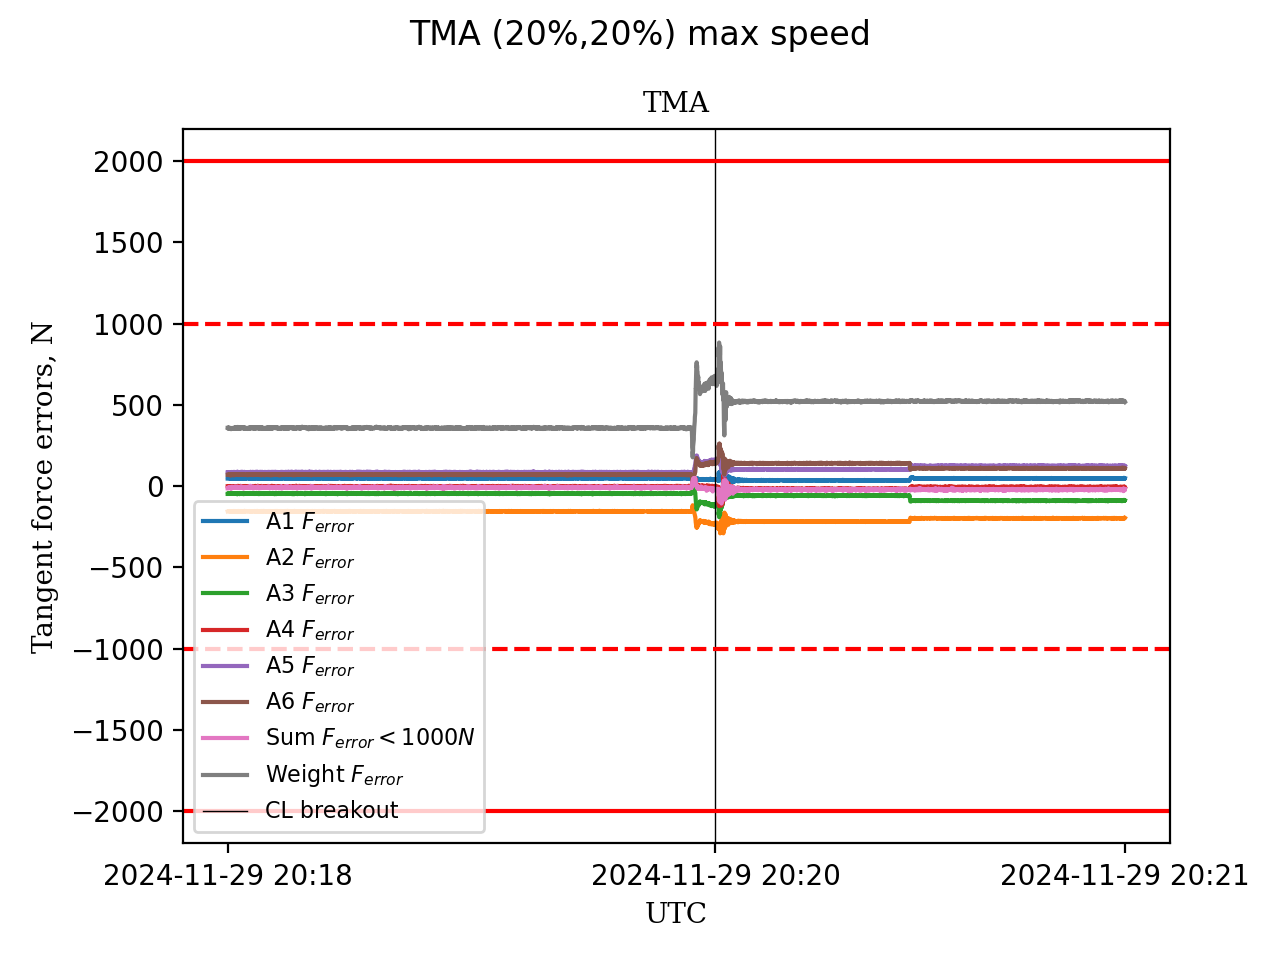
\includegraphics[width=0.8\textwidth]{spa/20_vel_acc_jerk/BLOCK-T241_m2_tangent_force_errors.png}
    \caption{M2 tangential force errors during the closed-loop break-out test.}
    \label{fig:block241_m2_tangent_force_errors}
    \end{figure}


\subsubsection{TMA azimuth and elevation brake tests}
\label{subsubsec:tma_azimuth_and_elevation_brake_tests}

The tests \testCase{BLOCK-T231} TMA Azimuth Brake Test and
\testCase{BLOCK-T240} TMA Elevation Brake Distance are designed to ensure that the
telescope will stop in case of an emergency. Accordingly to \figRef{block240_azEl_brake_distance}
the telescope travels 1.6 degrees in El (2.2 deg/s$^2$ peak deceleration) after the hard stop initiated.
In Az, it travels 1.9 degrees (3.9 deg/s$^2$ peak deceleration) after hard stop initiated.
Both without any mirror faults. These values seem reasonably low and confirm that the telescope
would be safe in case of an emergency.

\begin{figure}
  \centering
  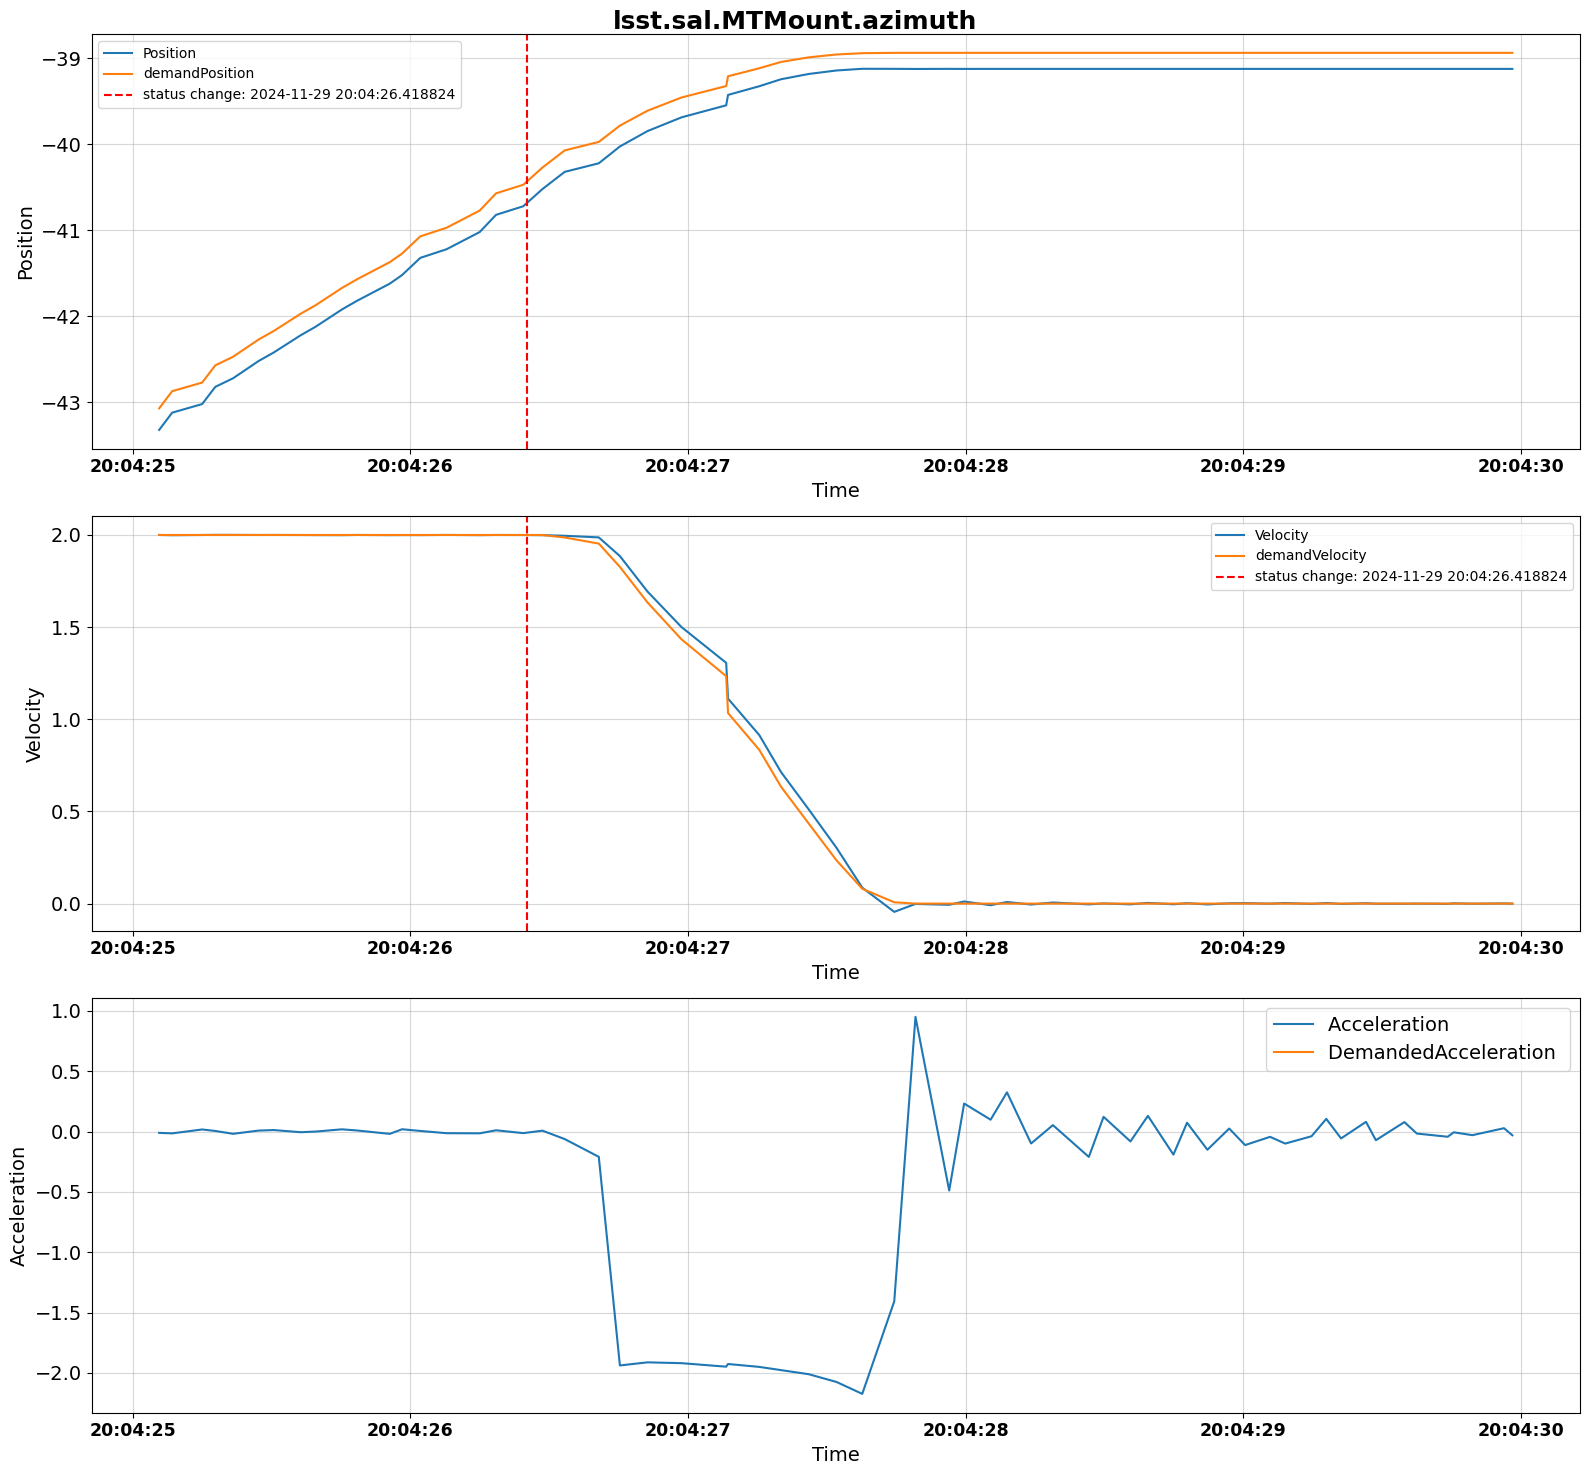
\includegraphics[width=0.45\textwidth]{spa/20_vel_acc_jerk/BLOCK-T231_az_brake_tests.png}
  \qquad
  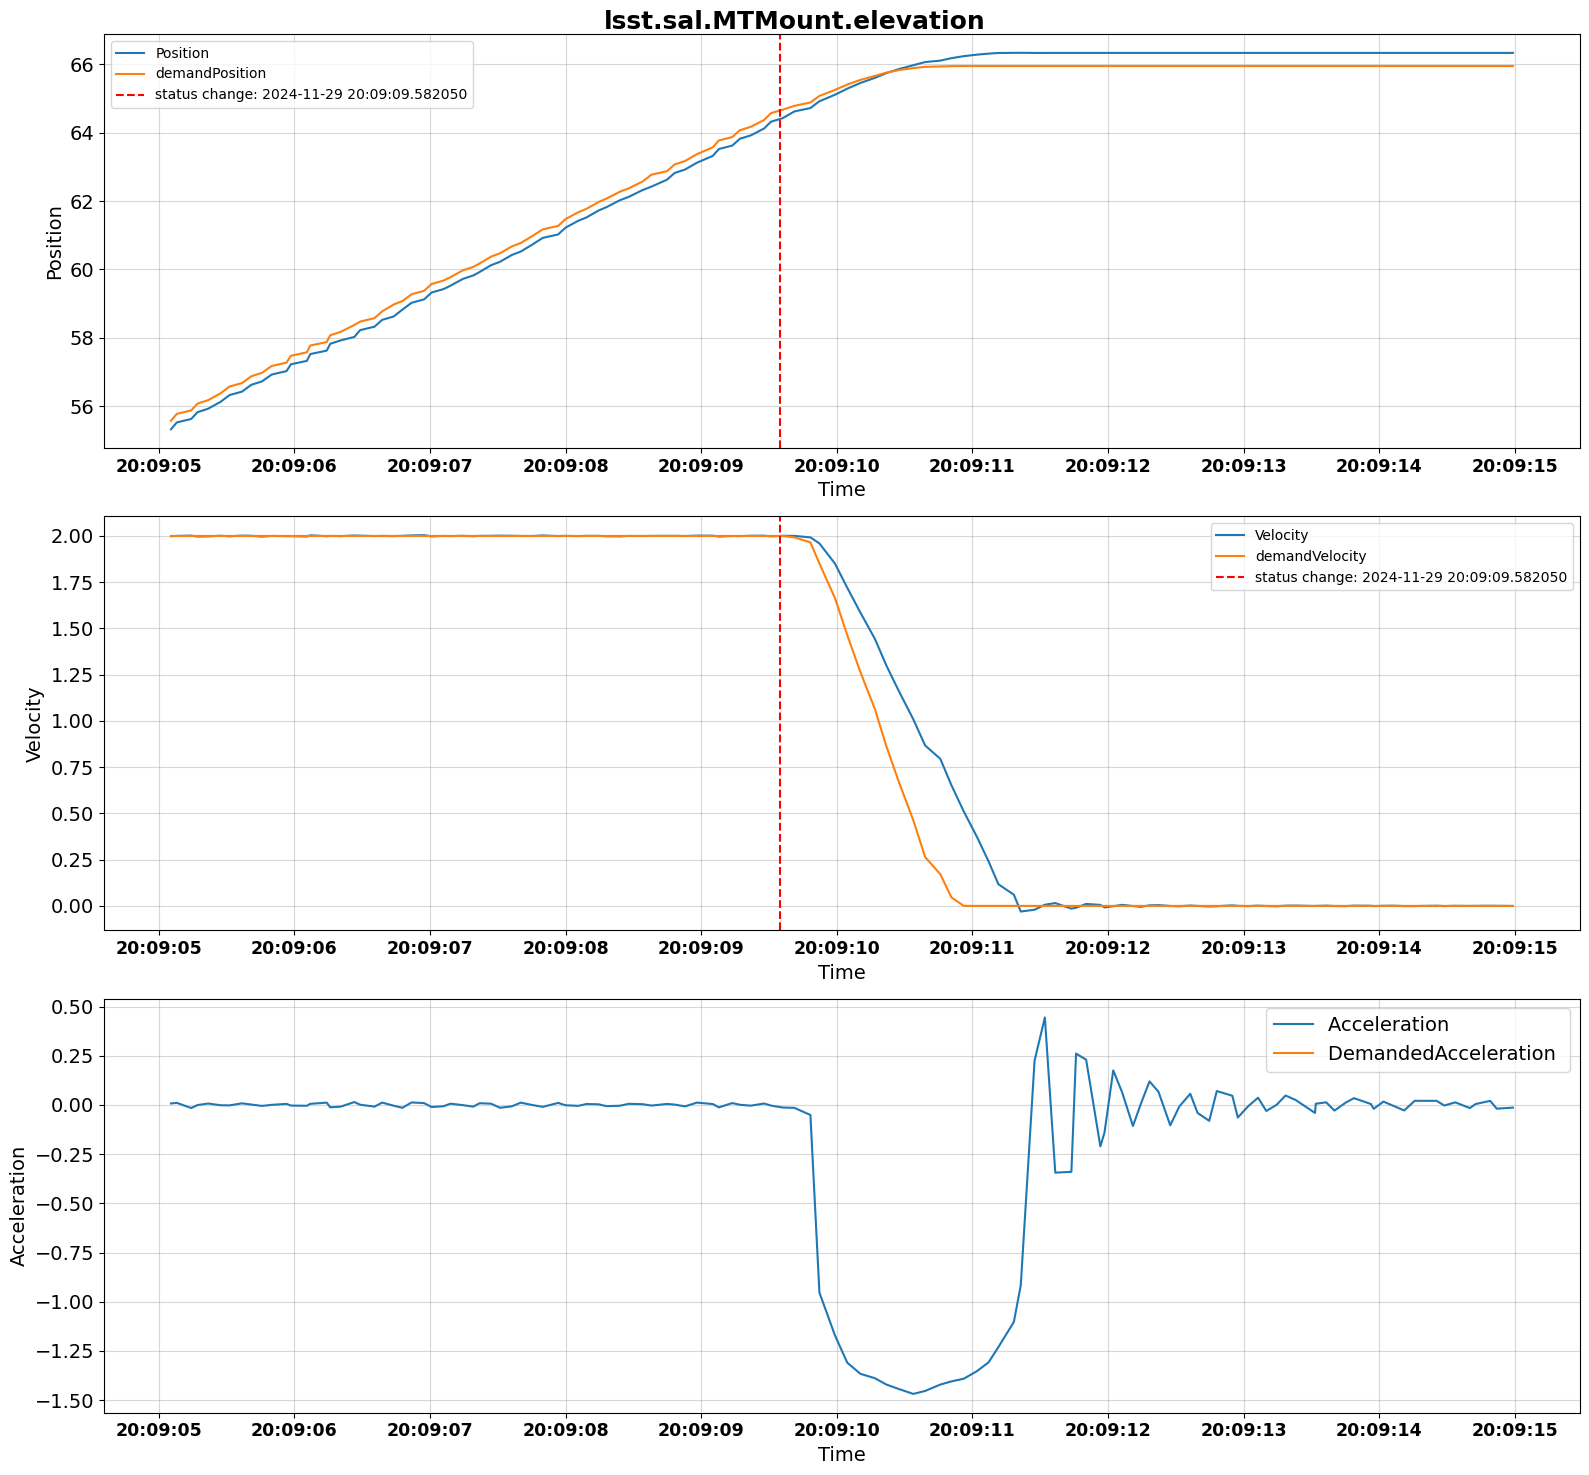
\includegraphics[width=0.45\textwidth]{spa/20_vel_acc_jerk/BLOCK-T240_el_brake_tests.png}
  \caption{TMA Brake Test in Azimuth (left) and Elevation (right).}
  \label{fig:block240_azEl_brake_distance}
\end{figure}

\subsection{Night Performance}

Statistical reports/summaries during the night?
\begin{itemize}
    \item Measured m1m3 hardpoint histograms min/max HP forces.
    \item FRACAS-158 / SITCOMTN-081 / SITCOM-1758 - Oscillations on HP forces and on azimuth torques
\end{itemize}


\section{Active Optics System Commissioning}
\label{sec:aos_commissioning}

The goals for commissioning of the AOS system with ComCam are to demonstrate that we can align the telescope optics, determine and correct for optical aberrations using the hexapods and bending modes for M2 and M1M3, and apply these corrections as a closed loop system. A stretch goal is to demonstrate that, for the limited field-of-view of ComCam, we can meet the image quality requirements of the LSST system (i.e., with the optical system delivering less than 0.4 arcseconds to the image quality budget) and do so consistently as a function of elevation and temperature. We have achieved many of these goals, but there are still significant challenges in delivering seeing limited images consistently as a function of variable observing conditions.

AOS commissioning started on 2024-10-24 with the first ComCam images delivering a 1.7 arcsecond full-width half-maximum (FWHM) image quality. This is a testament to the exceptional metrology work of the engineering and optical teams during assembly and to the optimization of the Look-Up Table (LUT) for all the active optics components using the  laser tracker data as well as mirror force balance data throughout 2024. 

Sub-arcsecond image quality was achieved on the night of 2024-11-06, with a best image quality of 0.66 arcsecond FWHM (with a 0.1 arcsecond variation across the field achieved) on the night of  2024-11-12. Corrections for the optical aberrations have been achieved using two independent approaches; the TIE wavefront estimation algorithm, which is an inversion method, and the Danish wavefront estimation algorithm, which is a forward modeling method. The AOS system was able to achieve closed-loop corrections across varying elevations and stellar densities, with most optical modes utilized (excluding the three highest-order modes on M2). Closed-loop operations have been run autonomously by the observing specialists to show that the scripts and procedures are mature. Preparations are underway to prototype a fully autonomous survey-mode triplet-taking block before the conclusion of ComCam's on-sky operations.

While we have demonstrated that Rubin can achieve the optical performance requirements for the AOS system there are significant challenges in meeting the optical performance requirements consistently as a function of temperature and elevation. It is not currently clear which aspects of the optical system are limiting its performance but the AOS team is working to understand the source of high levels of defocus and some amount of astigmatism that are present in the Zernike measurements. The team is also working to improve the computational efficiency of the system, which currently takes 5 minutes to complete a closed-loop iteration. 

After significant development, the AOS algorithms appear robust for a range of source densities and image qualities. A number of failure modes of the AOS software are present and being investigated. These include failures in processing images through Rapid Analysis when donuts cannot be detected on all sensors, and difficulty in measuring the wavefront when the images are significantly defocused (e.g., when the intra or extra focal images appear in focus). The AOS team is working to improve the robustness of the system to monitor these and other failure modes.

Figure~\ref{fig:aos} shows the FWHM delivered by the optical system (black line) as we correct the alignment and bending modes of the mirrors and camera over the nights 2024-11-25 to 2024-12-01. The FWHM is estimated from the Zernike amplitudes measured from out-of-focus donuts. The grey and blue lines are the 500nm and zenith corrected image qualities measured by SOAR and from the Rubin images respectively. The dashed green line is the 0.25 arcseconds image quality requirement for the telescope optics. From these measurements the AOS system is shown capable of meeting the image quality requirements. Delivering this consistently and without significant fine tuning is the current focus for the AOS team.

\begin{figure}
    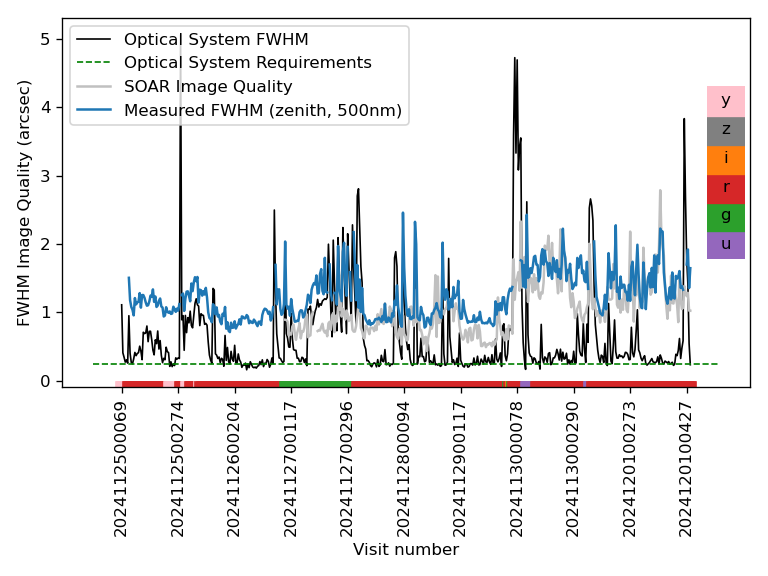
\includegraphics[width=0.7\textwidth]{figures/optical_performance.png}
    \caption{The FWHM delivered by Rubin (blue), the image quality from Rubin's optical system estimated from the AOS (black), and the  image quality measured by SOAR (gray). The Rubin and SOAR measured FWHMs are corrected to 500nm and zenith.}
\end{figure}

%z22 z11

\subsection{Initial Alignment}
Initial alignment of the AOS utilizes an updated laser tracker nominal frame based on a Final Element Analysis Model.  This ensures that the system is brought into focus prior to the start of observations.  Combined with a measurement of the impact of gravity on the telescope, these refinements simplified the alignment process, demonstrating the value of accurate laser tracker data. Once we were able to get on-sky images using curvature wavefront sensing, we finalized the initial state of the hexapods position to ensure a well aligned system at the start of the night. Work is ongoing to understand the stability of the initial hexapod and bending mode positions across nights to determine how well we can predict the  configuration of the AOS system at the start of each night. 


\subsection{Coordinate Systems}
During the first few weeks, significant effort was devoted to understanding and refining coordinate systems at different steps of the Active optics closed-loop process (wavefront sensor estimation and correction calculation). We conducted the test by introducing one degree of freedom at a time and correcting for it. We identified a rotation discrepancy in ComCam's installation compared to the expected design, requiring 
adjustments in our alignment procedures. The coordinate discrepancies were resolved empirically in the early AOS tests. Based on these data the expected as-delivered coordinate system(s) for the mirrors, hexapods, and sensors will need to be derived from first principles and validated prior to AOS observations with LSSTCam.


\subsection{Wavefront estimation}
The wavefront estimator proved robust across diverse observing conditions of seeing, mount elevation and a few filters (r,i and y band) 
On dense fields such as 47 Tuc or NGC 253, the estimator provided accurate results for  all sensors except the central one.  Comparison of observed PSFs with simulations  confirmed the  accuracy of Rubin's ray-tracing software, \texttt{Batoid}.

Wavefront estimation and closed-loop convergence has been demonstrated using \texttt{TIE} and \texttt{Danish}. Other advancements include the implementation of sparse Zernikes,  allowing selective inclusion of Zernike polynomial terms while minimizing cross-contamination 
of modes with identical azimuthal dependencies.

Despite delivering good optical quality, Zernike measurements indicate persistently high levels of defocus and some amount of astigmatism. We are continuing to investigate the source and impact of these measurements.

\subsection{Closed Loop}
Following resolution of initial issues with the AOS pipelines,  closed-loop operations were achieved across varying elevations and filters (u, g, r, i, z, and y).  Most optical modes were utilized, excluding the three highest-order modes on M2.  Consistency in results across nights confirmed the need for further refinement of the LUT. In favorable seeing conditions, the system achieved sub-arcsecond image quality, with FWHM as low as 0.65 arcseconds. Autonomous closed-loop operations were run by observers, demonstrating the maturity of the system. 

%Zernike-based AOS FWHM  contributions confirmed the system's convergence to exceptional image quality. 

The closed loop process still takes 5min  often requiring 5 or more iterations. The best performance for the closed loop achieved convergence in two iterations but delivering this consistently has not been achieved and tuning the closed-loop gain and making further adjustments to improve computational  efficiency remains a priority for the team.

\subsection{LUT}
The LUT underwent initial validation across elevations, azimuths, and rotator angles, 
leading to incremental improvements. While these updates enhanced performance, 
further refinements are needed to address second-order dependencies. Insights 
from ComCam data will inform these efforts, ensuring readiness for LSSTCam, which 
may present distinct challenges due to its larger focal plane and optical system.



\subsection{Lessons Learned and Next Steps}
\textbf{Lessons Learned}
- Coordinate Systems: Precision and methodical testing of coordinate systems are essential. 
Starting with foundational tests and incrementally increasing complexity ensures reliability.
- Observer Training: Comprehensive documentation, including a subsystem overview and closed-loop procedures, 
significantly enhances observer support capabilities.
- Closed-Loop Performance: Iterative testing and tuning of the closed-loop system are essential for delivering a consistently high image quality as a function of temperature, elevation, and other observing conditions. Achieving this performance consistently and without significant fine tuning will be a significant challenge.
- Engagement and Morale: Fun and engaging night summaries boost team morale, fostering a collaborative 
and motivated work environment.
- Transferability: Some ComCam lessons learned, particularly LUT and coordinate system adjustments, 
will not fully transfer to LSSTCam, requiring repeated validation.

\textbf{Next Steps}
- Conduct step-by-step closed-loop validations for LSSTCam, validating signs and rotations for intentional perturbations.
- Collaborate with the Camera Team to anticipate and mitigate known camera tilts.
- Implement and validate tests tailored to LSSTCam's larger focal plane dimensions.
- Prepare RubinTV and donutViz for full-array LSSTCam mode and automate its execution for all triplet-taking sequences.
- Adapt MTAOS to run as a continuous background task, supporting survey-mode operations.
- Optimize the AOS pipeline for speed, including binning and ISR performance improvements.




\subsection{Image Quality}
\label{sec:image_quality}

The AOS team has delivered very impressive image quality, showing images with 0.68 arcsec FWHM. If we assume
that sources of image degradation add in quadrature and we trust our estimates of atmospheric seeing, this is
consistent with reaching the image quality error budget allocation of our full system of 0.400 arcsec.

The best image quality achieved so far is \c 0.65 arcsec, with a median of 1.1 arcsec during science visits;
\tabRef{psf_summary}, \figRef{seeing_plot}, and \figRef{psf_fwhm_distribution}.

\begin{figure*}
  \centering
  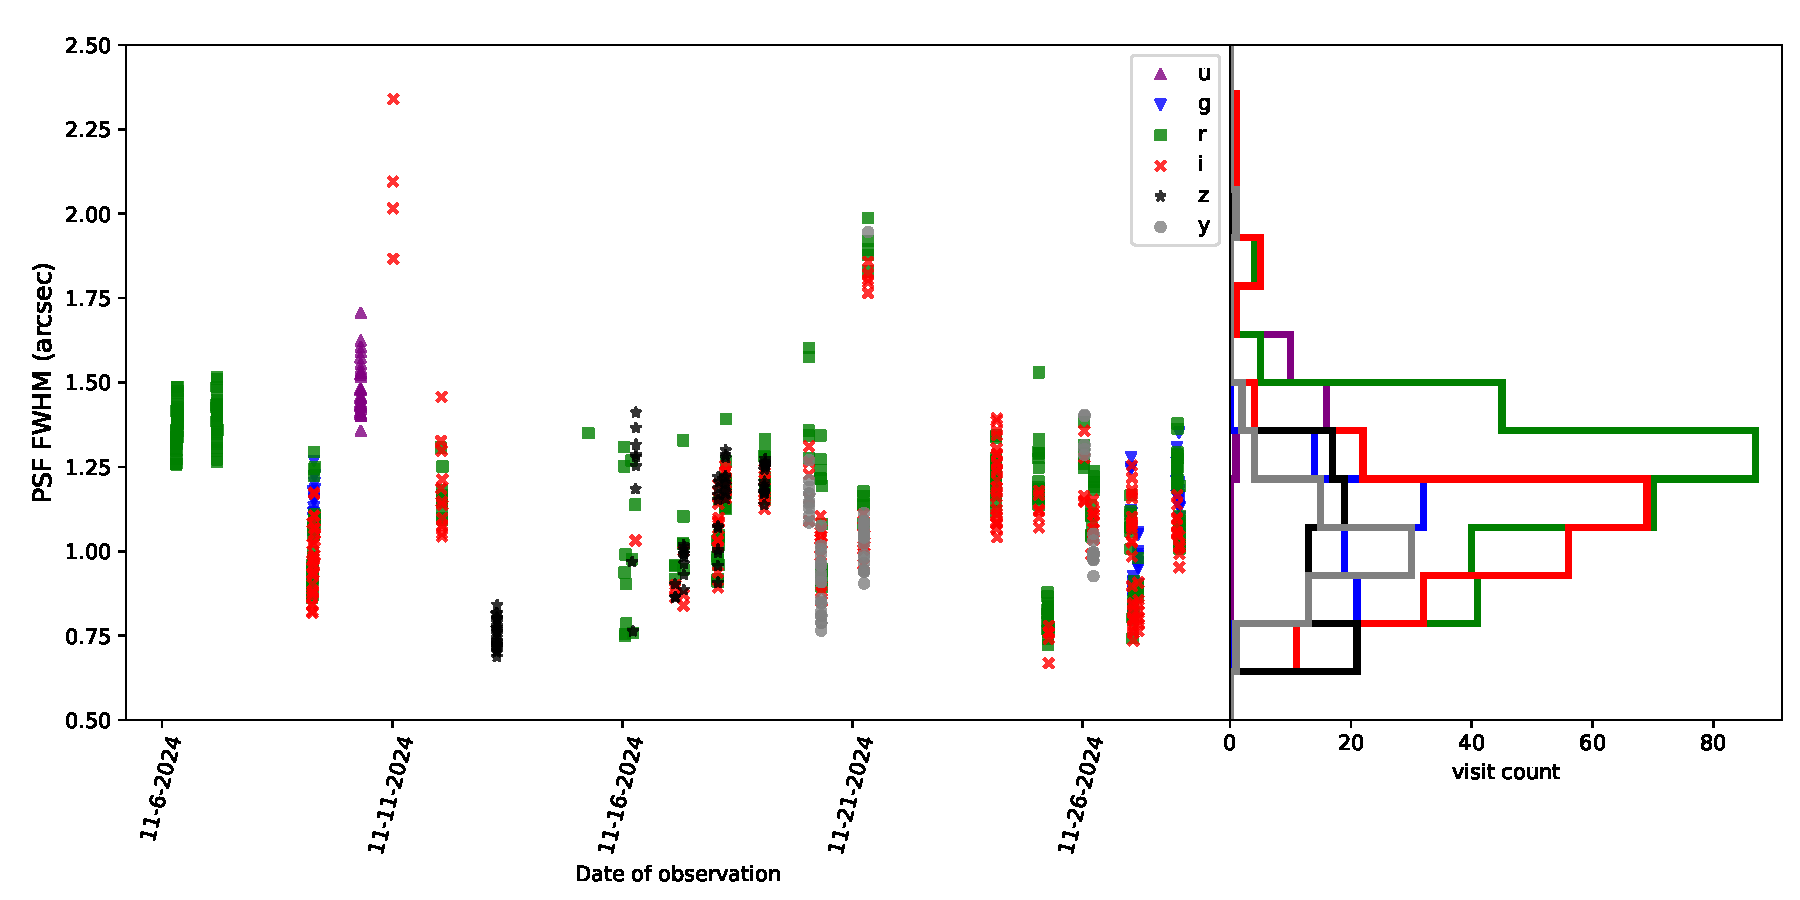
\includegraphics[width=\textwidth]{figures/seeing}
  \caption{\small PSF FWHM as a function of the observed date. Data are from DRP from 2024-11-01 to 2024-11-28.}
  \label{fig:seeing_plot}
\end{figure*}


\begin{table*}
\centering
\begin{tabular}{@{}lccc@{}}
\textbf{Band} & \textbf{Number of Visits} & \textbf{Mean PSF FWHM} & \textbf{STD. DEV. PSF FWHM} \\
 & & \textit{arcsec} & \textit{arcsec} \\
  \hline
All           & 775                      & 1.12                   & 0.23                  \\
u             & 28                       & 1.49                   & 0.08                  \\
g             & 86                       & 1.07                   & 0.14                  \\
r             & 307                      & 1.18                   & 0.22                  \\
i             & 203                      & 1.09                   & 0.24                  \\
z             & 85                       & 1.01                   & 0.21                  \\
y             & 66                       & 1.04                   & 0.18                  \\
\end{tabular}
\caption{Summary of PSF FWHM performance. Data are from DRP from 2024-11-01 to 2024-11-28.}
\label{tab:psf_summary}
\end{table*}

\begin{figure*}
  \centering
  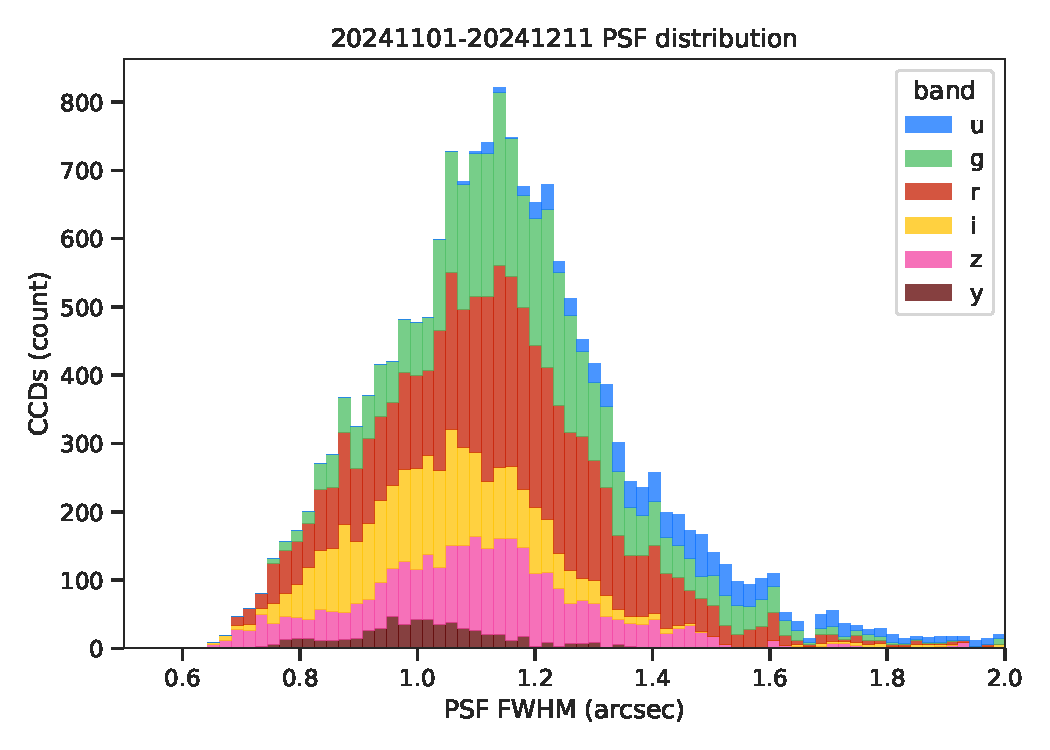
\includegraphics[width=0.7\textwidth]{image_quality_figures/comcam_science_psf_fwhm_hist.pdf}
  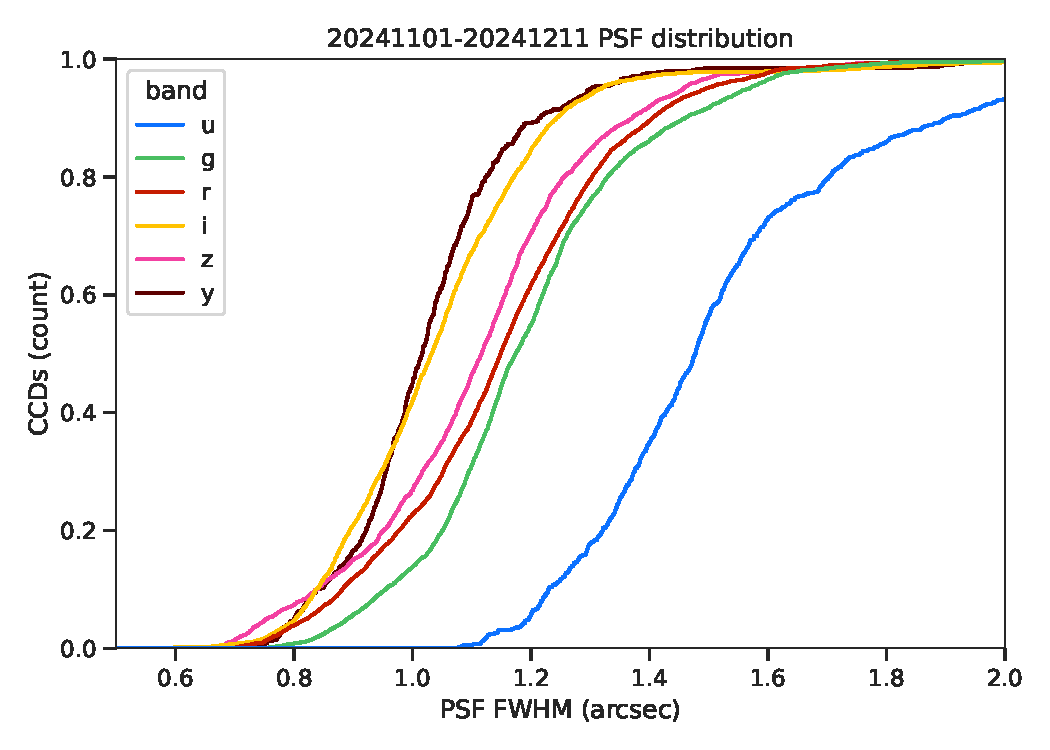
\includegraphics[width=0.7\textwidth]{image_quality_figures/comcam_science_psf_fwhm_cdf.pdf}
  \caption{Distribution of PSF FWHM represented as a histogram (top) and cumulative distribution (bottom).
  Data are from DRP from 2024-11-01 to 2024-12-11.}
  \label{fig:psf_fwhm_distribution}
\end{figure*}

We are in the process of quantifying the different sources of image degradation. The main ones we're focused on measuring are degradation due to the camera/instrument, static optics, dynamic optics, mount motion, and observatory seeing.

\subsubsection{Atmospheric Seeing}

We do not currently have a working Rubin DIMM, although repairs are in progress. In the meantime, we have a livestream of data from the SOAR \RINGSS.\footnote{A  next-generation DIMM developed by Andrei Tokovinin and Edison Bustos} We are working on getting direct access to current and historical data for \RINGSS as well as the Gemini DIMM.

\subsubsection{Static Optics}

See \secRef{aos_commissioning} for more details on the performance of the static optics system.

\subsubsection{Dynamic Optics}

Dynamic optics contributions are caused by oscillations or motion of the mirrors, causing the quality of the
optical alignment to change during an exposure. We have accelerometers in the mirror cell and on the top end
but have not yet analyzed the data.

\subsubsection{Observatory Seeing}

The two main contributors to observatory seeing are dome seeing and mirror seeing. We do not have a direct dome seeing monitor but we do have a 3D sonic anemometer located in the dome that is taking data. Larom Segev has looked at the correlation between the standard deviation of the sonic temperature, which should be a proxy for dome seeing due to thermal turbulence, and measured PSF FWHM in the science images (see \figRef{anemometer}). There may be some correlation, but we need more and better data, and to remove atmospheric seeing contributions.

\begin{figure}
  \begin{center}
    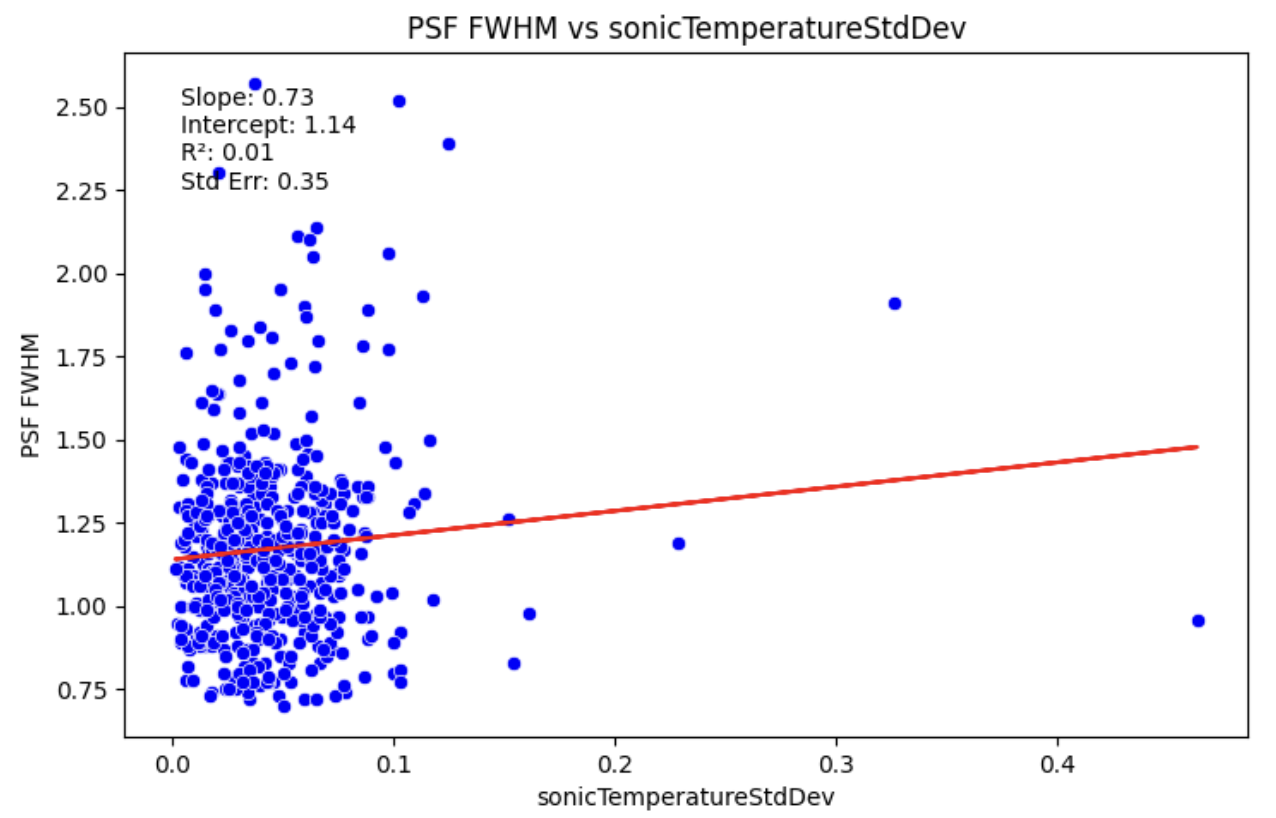
\includegraphics[width=0.6\textwidth]{image_quality_figures/anemometer_PSF.png}
  \end{center}
  \caption{PSF FWHM versus the standard deviation of sonic temperature.}
  \label{fig:anemometer}
\end{figure}

\subsubsection{Mount Motion}

There are two main components to image degradation due to mount motion. The first component comes from drift due to tracking errors. As we have not yet completed a full pointing model at all azimuths and elevations, we have not quantified this component yet. The second component of mount motion image degradation is due to tracking jitter. We quantify this by computing the rms deviation of the mount position as measured by the encoders from the position sent by MTPtg. Craig Lage computed the tracking jitter for all ComCam exposures through the 20th of November. From a total of 5311 images, the median image quality impact is 0.004 arcseconds, and 0.38\% of images have an impact to image quality of above 0.05 arcseconds (see \figRefIII{jitter}{jitter_1}{jitter_2}). This is well below the budgeted mount jitter error of 0.069 arcsec.

\begin{figure}
  \begin{center}
    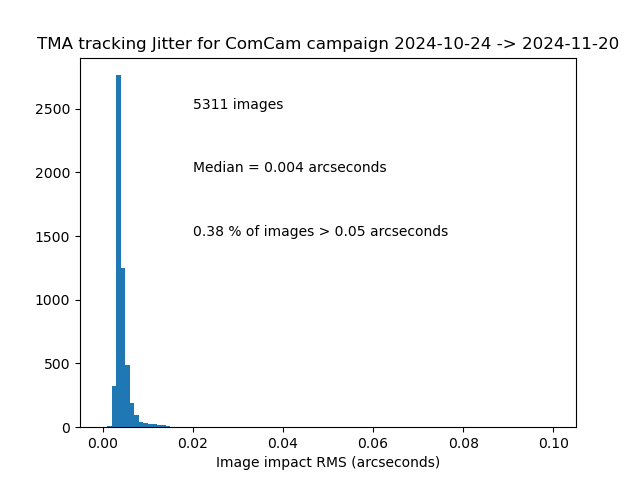
\includegraphics[width=0.8\textwidth]{image_quality_figures/ComCam_Mount_Jitter_21Nov24.png}
  \end{center}
  \caption{Total TMA tracking jitter for all exposures from October 24 to November 20.}
  \label{fig:jitter}
\end{figure}

\begin{figure}[ht]
    \centering
    \begin{minipage}{0.49\textwidth}
        \centering
        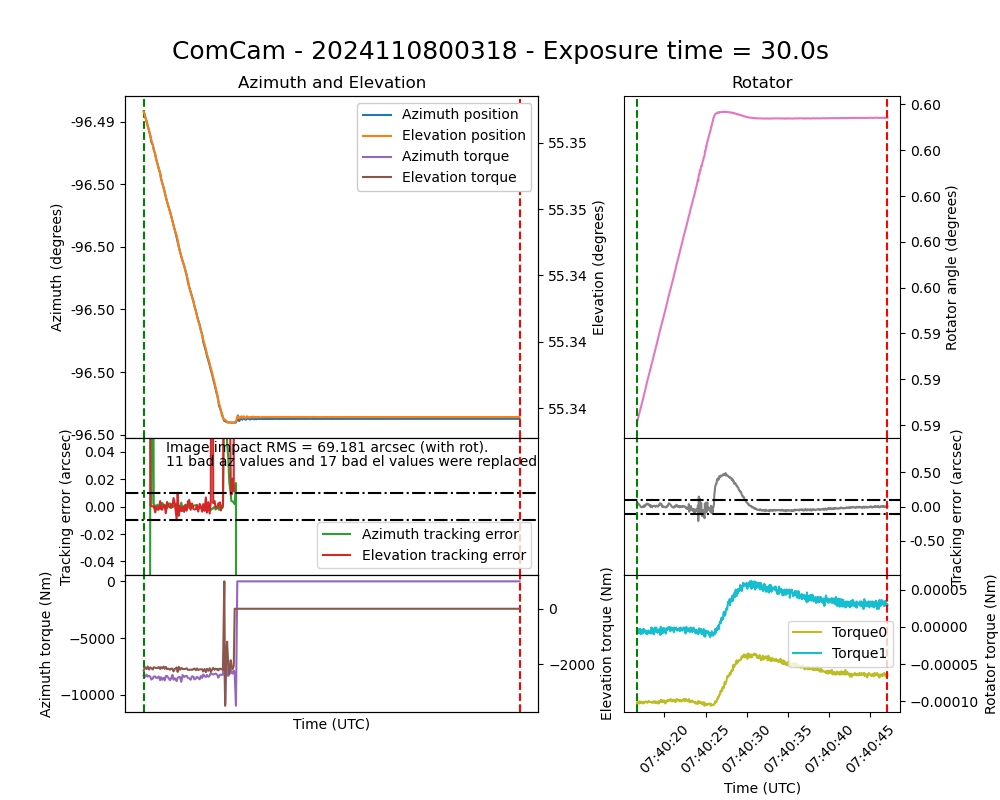
\includegraphics[width=\linewidth]{image_quality_figures/ComCam_Mount_Plot_2024110800318.png}
        \caption{Exposure with an unusually large amount of mount motion image degradation.}
        \label{fig:jitter_1}
    \end{minipage}\hfill
    \begin{minipage}{0.49\textwidth}
        \centering
        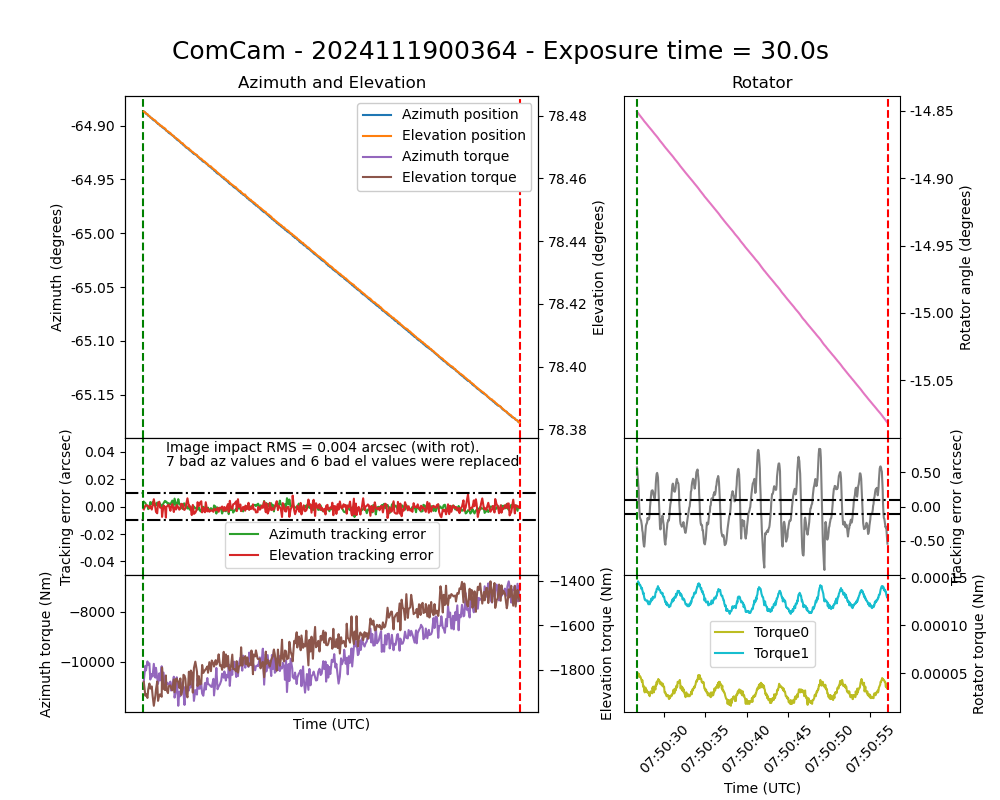
\includegraphics[width=\linewidth]{image_quality_figures/ComCam_Mount_Plot_2024111900364.png}
        \caption{Exposure with a typical amount of mount jitter.}
        \label{fig:jitter_2}
    \end{minipage}
\end{figure}

\section{Data Production}
\label{sec:data_production}

\section{Calibration Data}
\label{sec:calibration_date}

\subsection{Twilight Flats}

Because the flat field screen and illuminator is not expected to be operational while ComCam is on the telescope, we used dithered, tracked twilight flats to generate the combined flat calibration frames. The exposure time of the twilight flats were dynamically adjusted to hit a target count, generally in the range of 10-20k. The flats taken at a wide range of azimuth angles and rotator angles. See Fig.~\ref{fig:twilight_counts} for the counts per pixel per second as a function of sun elevation angle.

\begin{figure}
  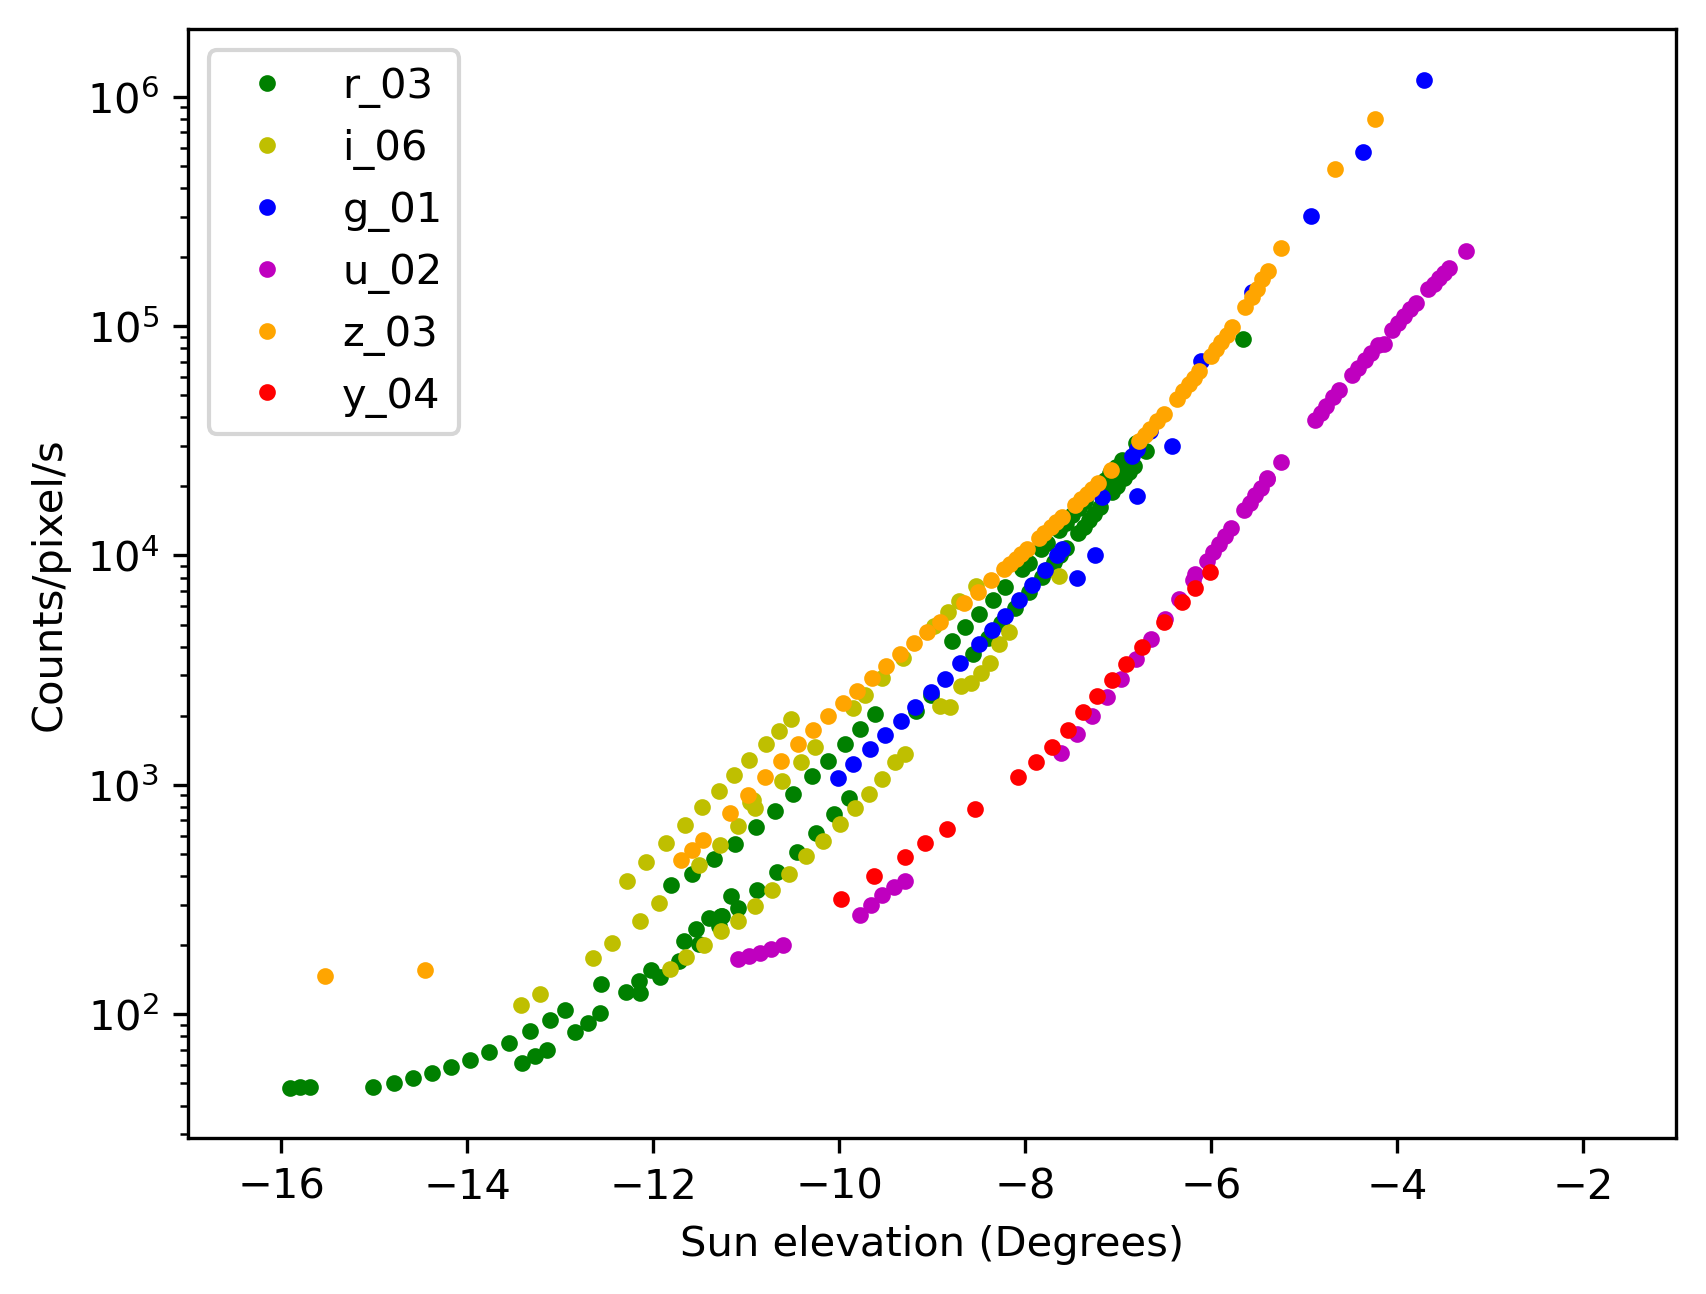
\includegraphics{calibration_data_figures/twilight_flat_counts.png}
  \caption{Twilight flat counts per pixel per second for each filter as a function of sun elevation angle.}
  \label{fig:twilight_counts}
\end{figure}
  

\section{Science Pipelines Commissioning Observations}
\label{sec:science_pipelines_commissioning_observations}

\section{Throughput for Focused Light}
\label{sec:throughout_for_focused_light}

The ComCam throughput has been estimated in ugriz using FGCM and is discussed in detail in Sec.~\ref{sec:photometric_calibration}.

\subsection{Collimated Beam Projector Status}

The Collimated Beam Projector (CBP) and Ekspla tunable laser were both installed on the dome during the week
of November 18. See Figs.~\ref{fig:cbp_1}, \ref{fig:cbp_2}, \ref{fig:laser} They will both be connected to ethernet and a laser interlock system will be installed. First photon from the CBP is projected for December 2.

\begin{figure}[htbp]
  \includegraphics[width=\textwidth]{throughput_for_focused_light_figures/cbp_on_dome_1.png}
  \caption{Image of the CBP, which was installed on the dome on November 22.}
  \label{fig:cbp_1}
\end{figure}
  
\begin{figure}[htbp]
  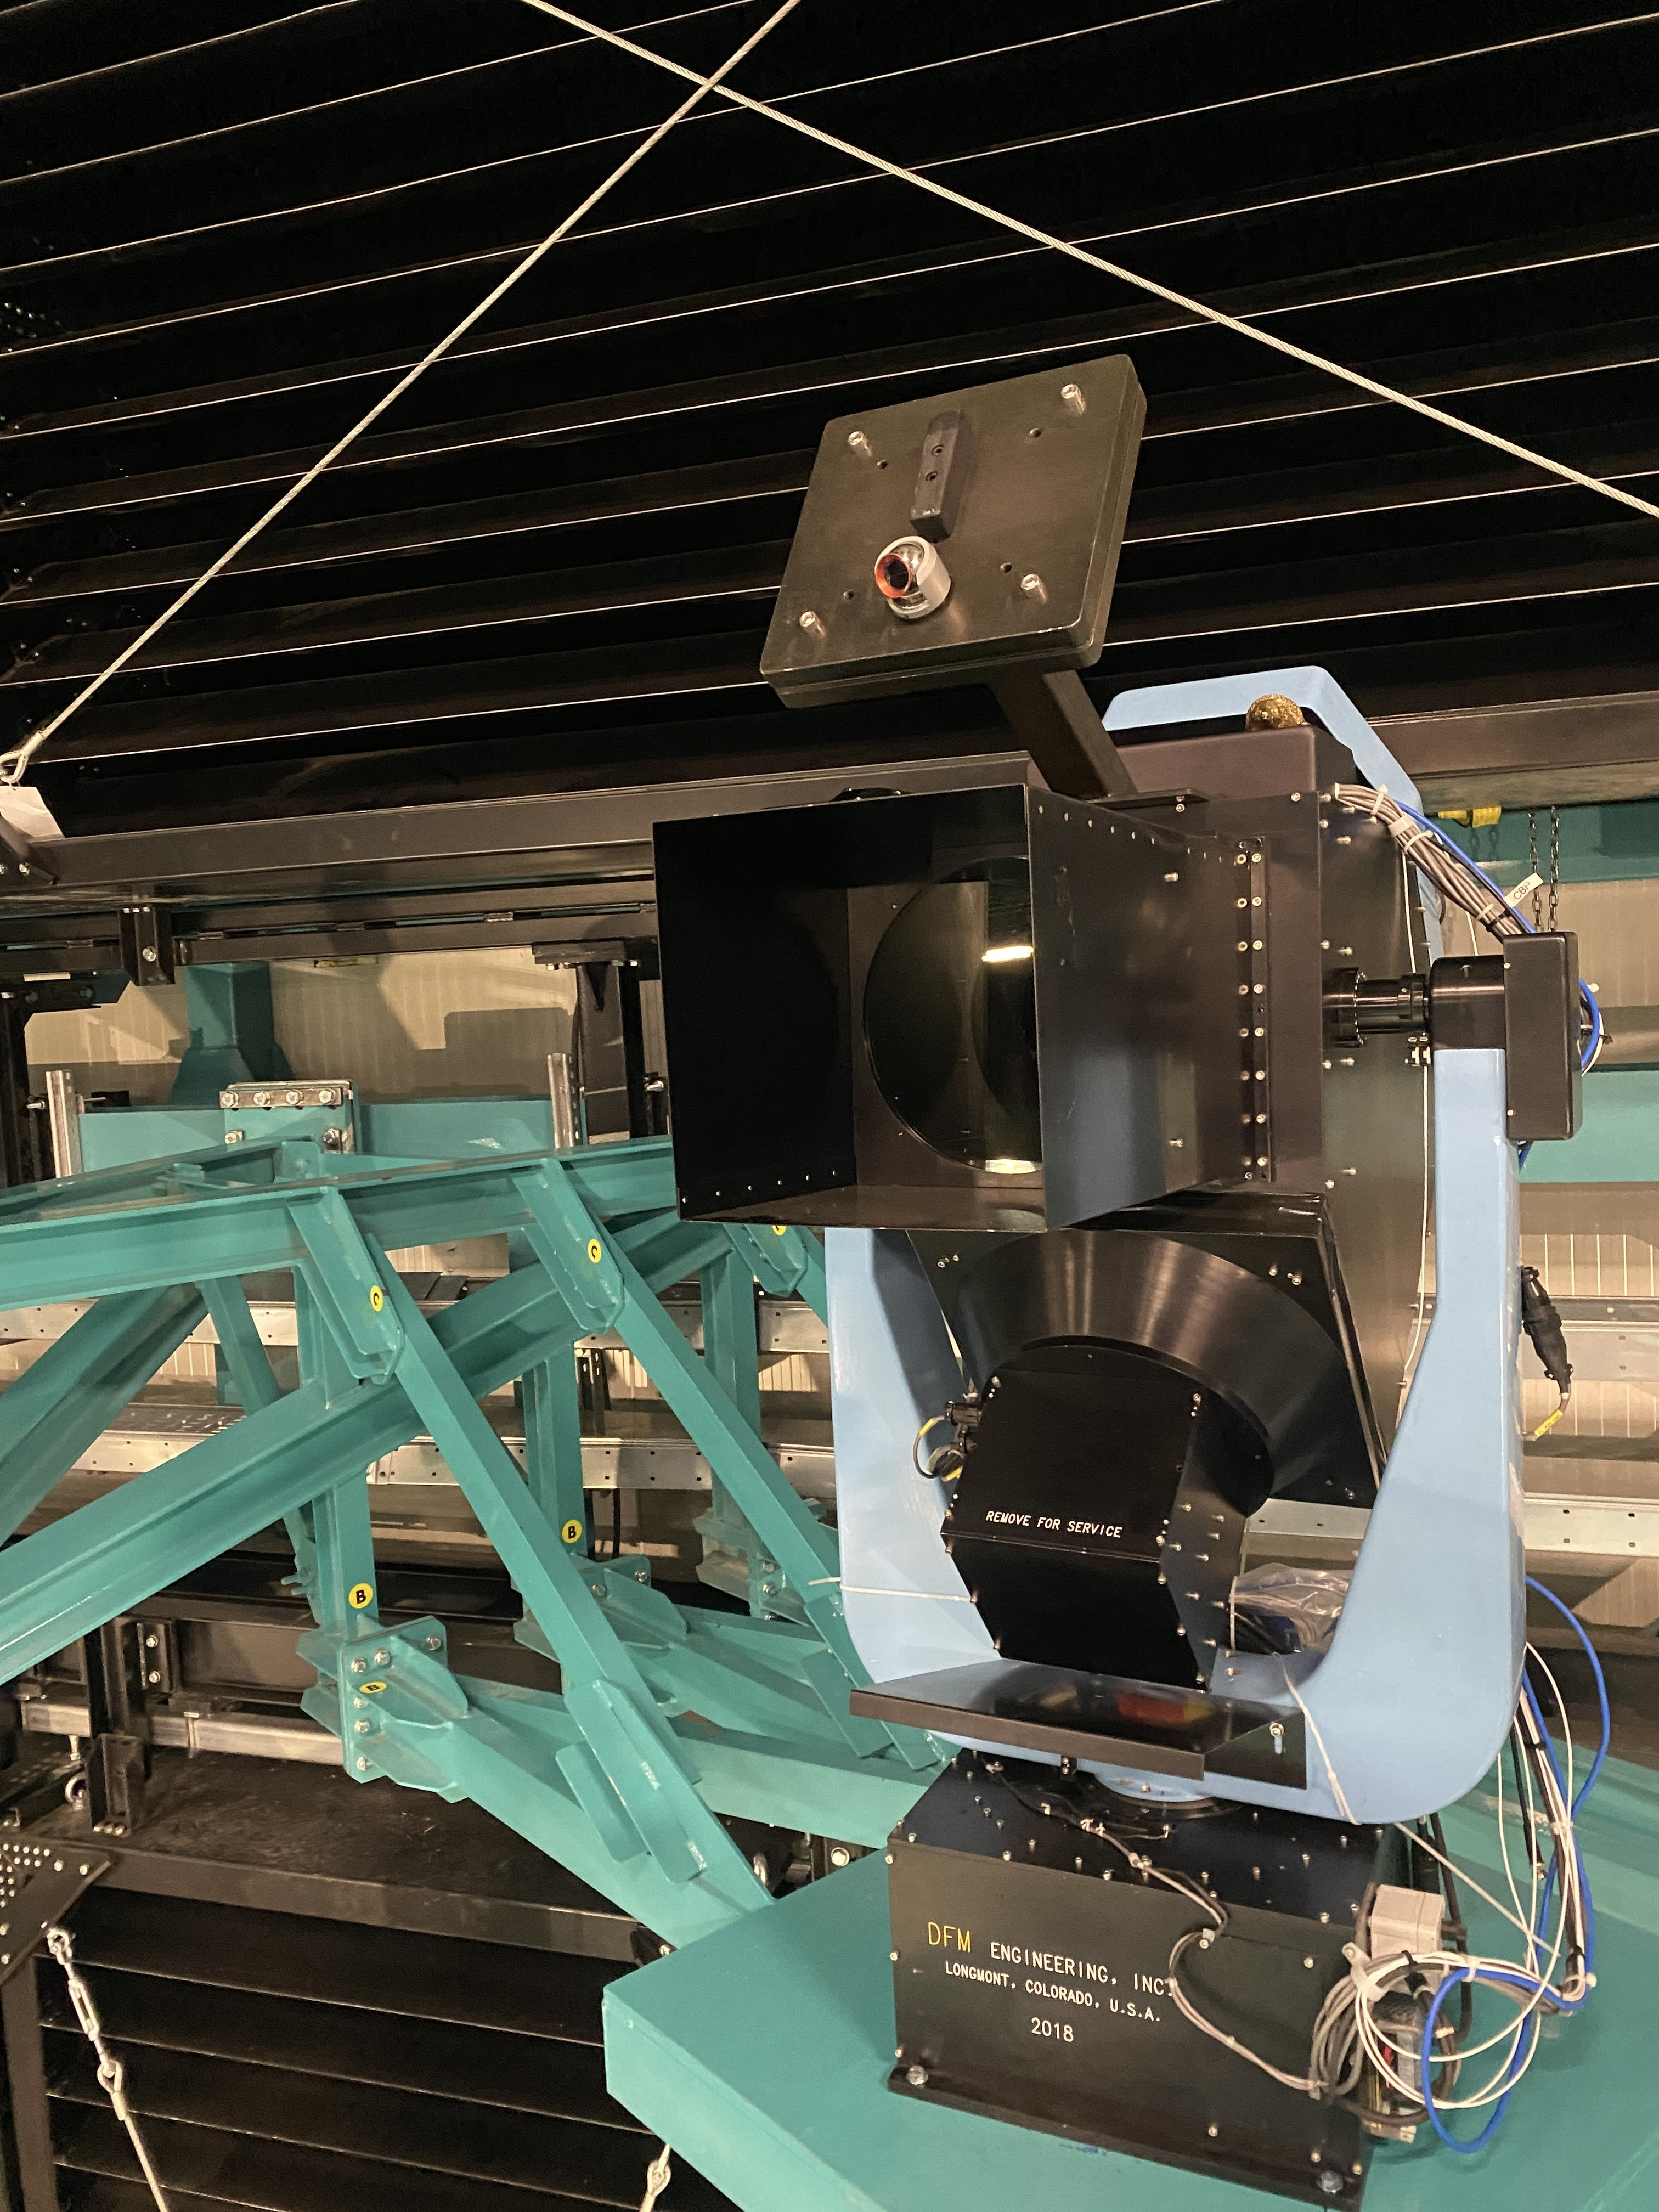
\includegraphics[width=\textwidth]{throughput_for_focused_light_figures/cbp_on_dome_2.png}
  \caption{Image of the CBP, which was installed on the dome on November 22.}
  \label{fig:cbp_2}
\end{figure}
  
\begin{figure}[htbp]
  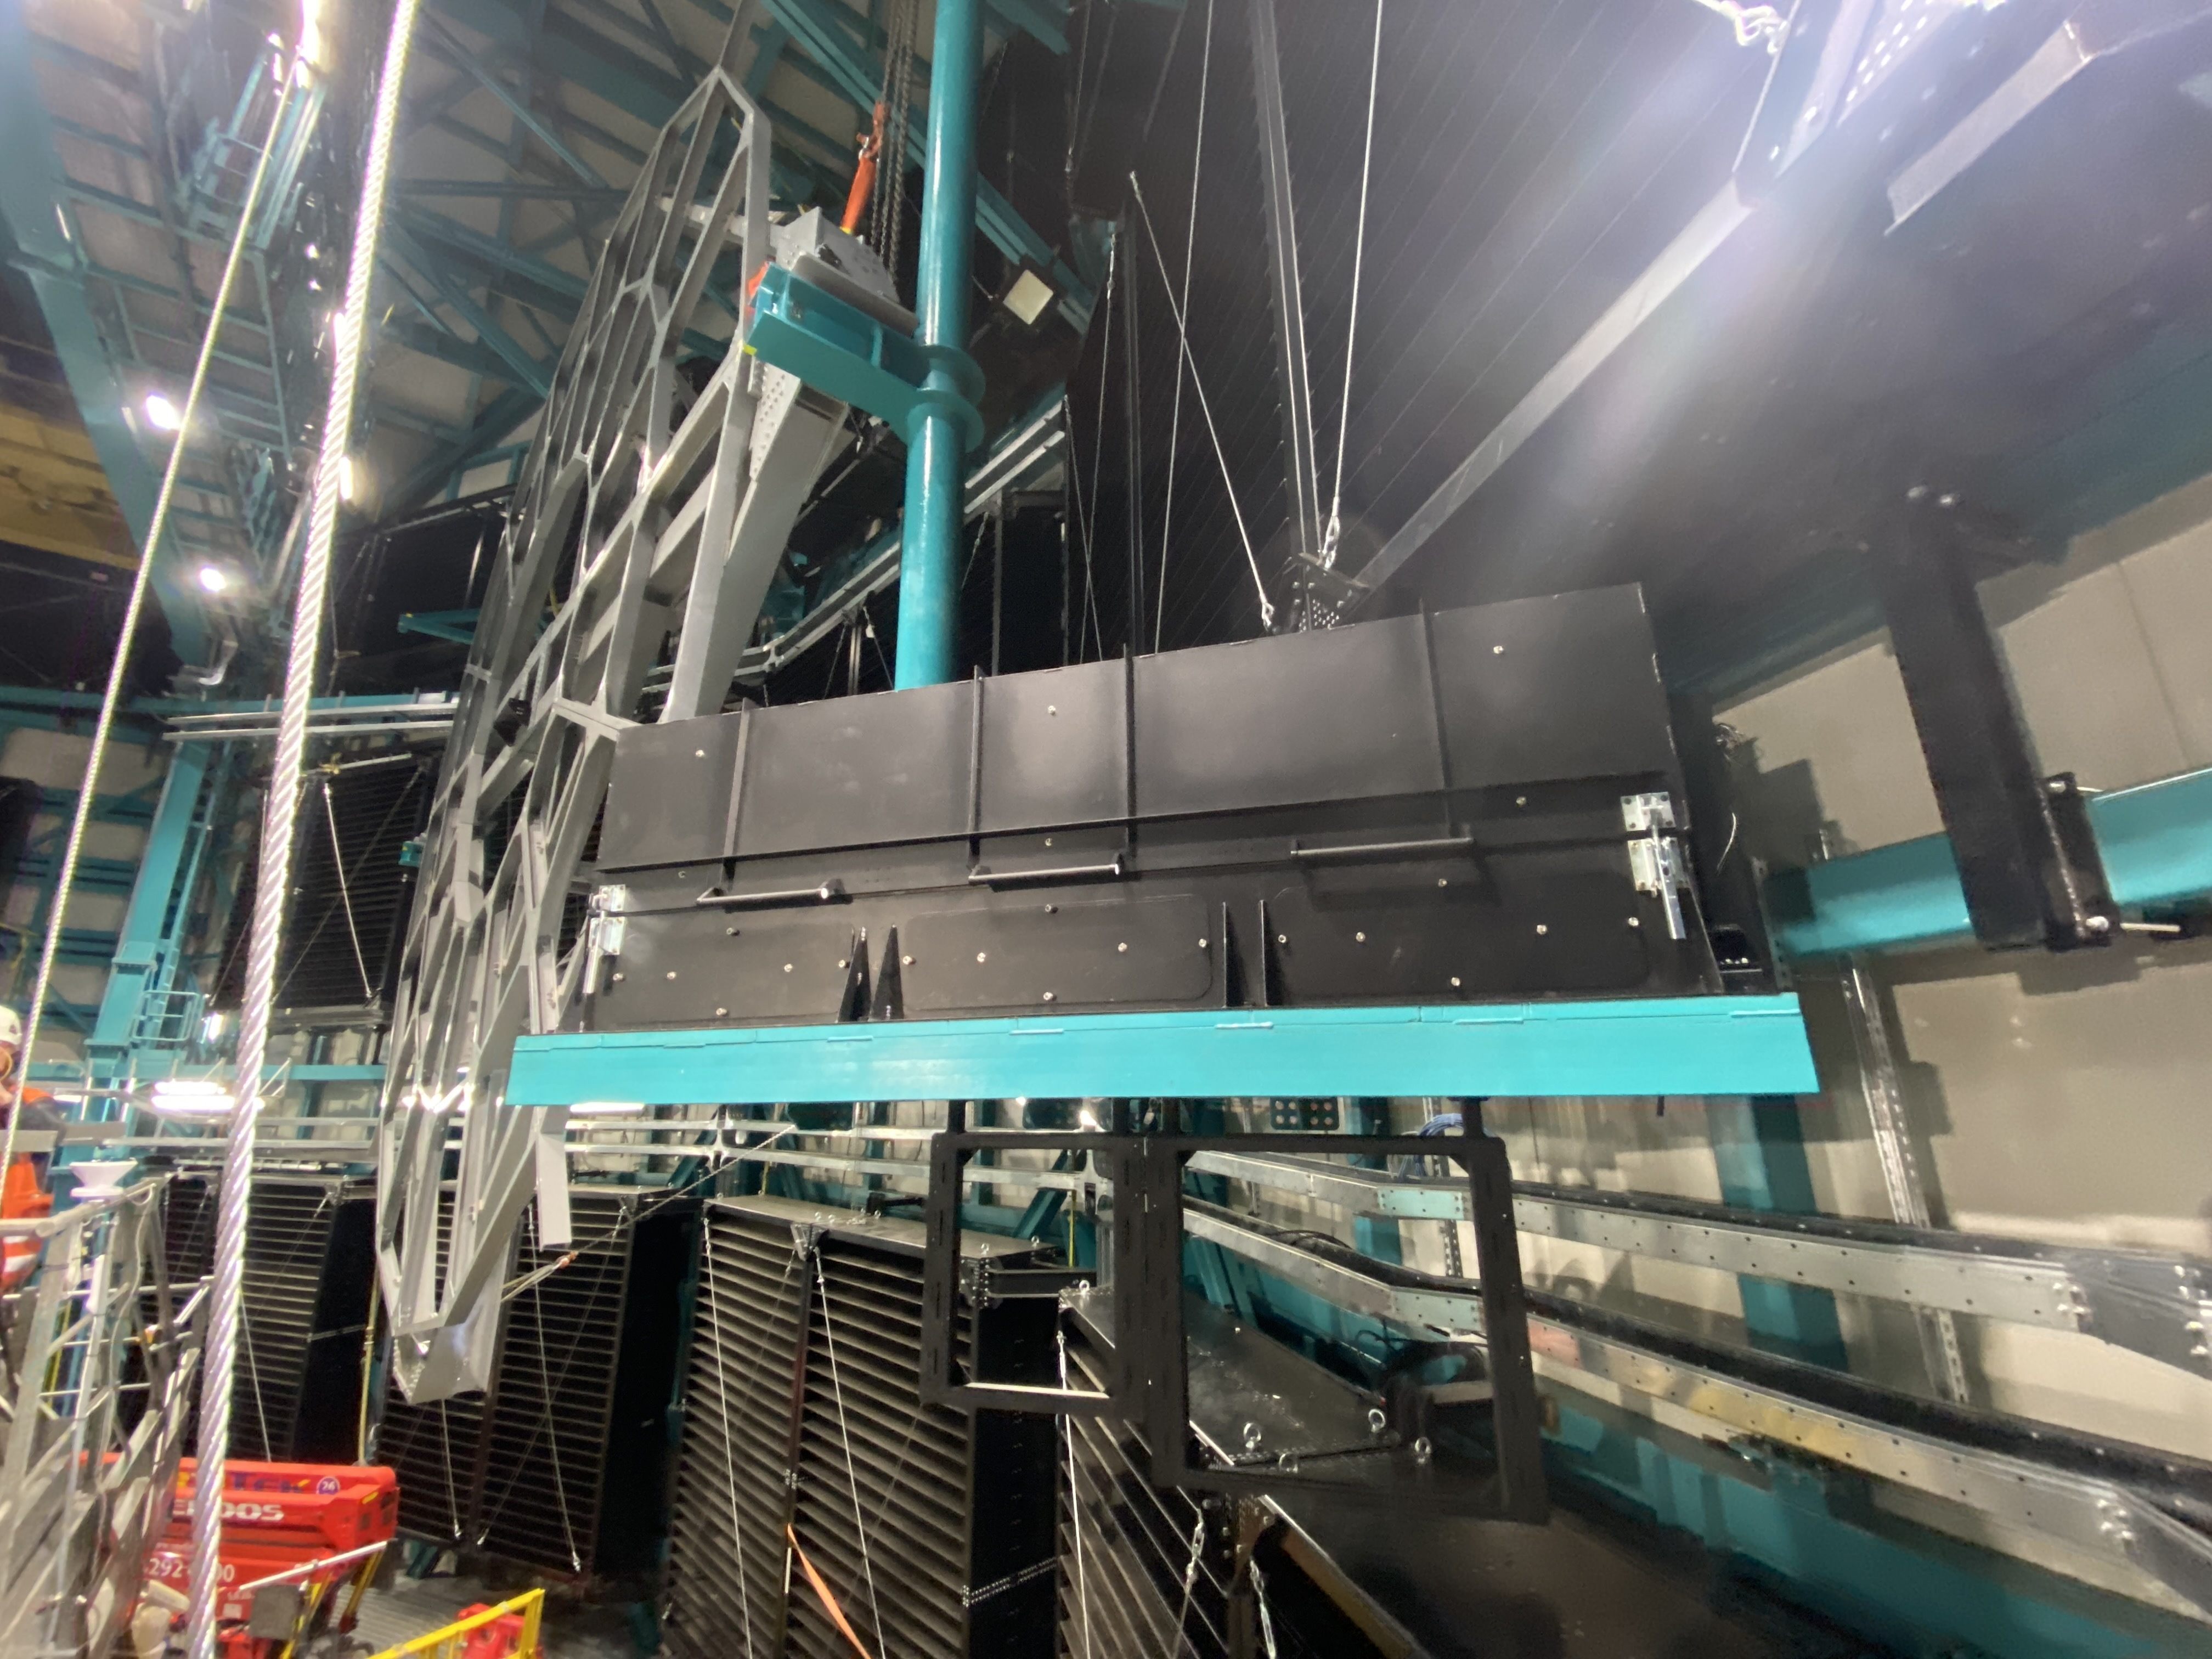
\includegraphics[width=\textwidth]{throughput_for_focused_light_figures/laser_on_dome.png}
  \caption{Image of the laser box, containing the Ekspla tunable laser, which was installed on the dome on November 21.}
  \label{fig:laser}
\end{figure}

\subsection{Delivered Image Quality and PSF}
\label{sec:delivered_image_quality_and_psf}


Image quality and PSF modeling are closely tied to the progress of the AOS system, and here is what can be concluded halfway through the data gathering with \ComCam.

\subsubsection{On Image Quality}

The best image quality achieved so far is 0.7 arcsec, with a median of 1.1 arcsec during science visits. As shown in Table \ref{tab:psf_summary} and Figure \ref{seeing_plot}, the PSF FWHM as a function of observation dates highlights the progress. It is important to note that all these data were collected during the AOS testing and validation phase. This makes the achieved image quality even more encouraging, demonstrating significant progress.

\begin{figure*}
        \centering
        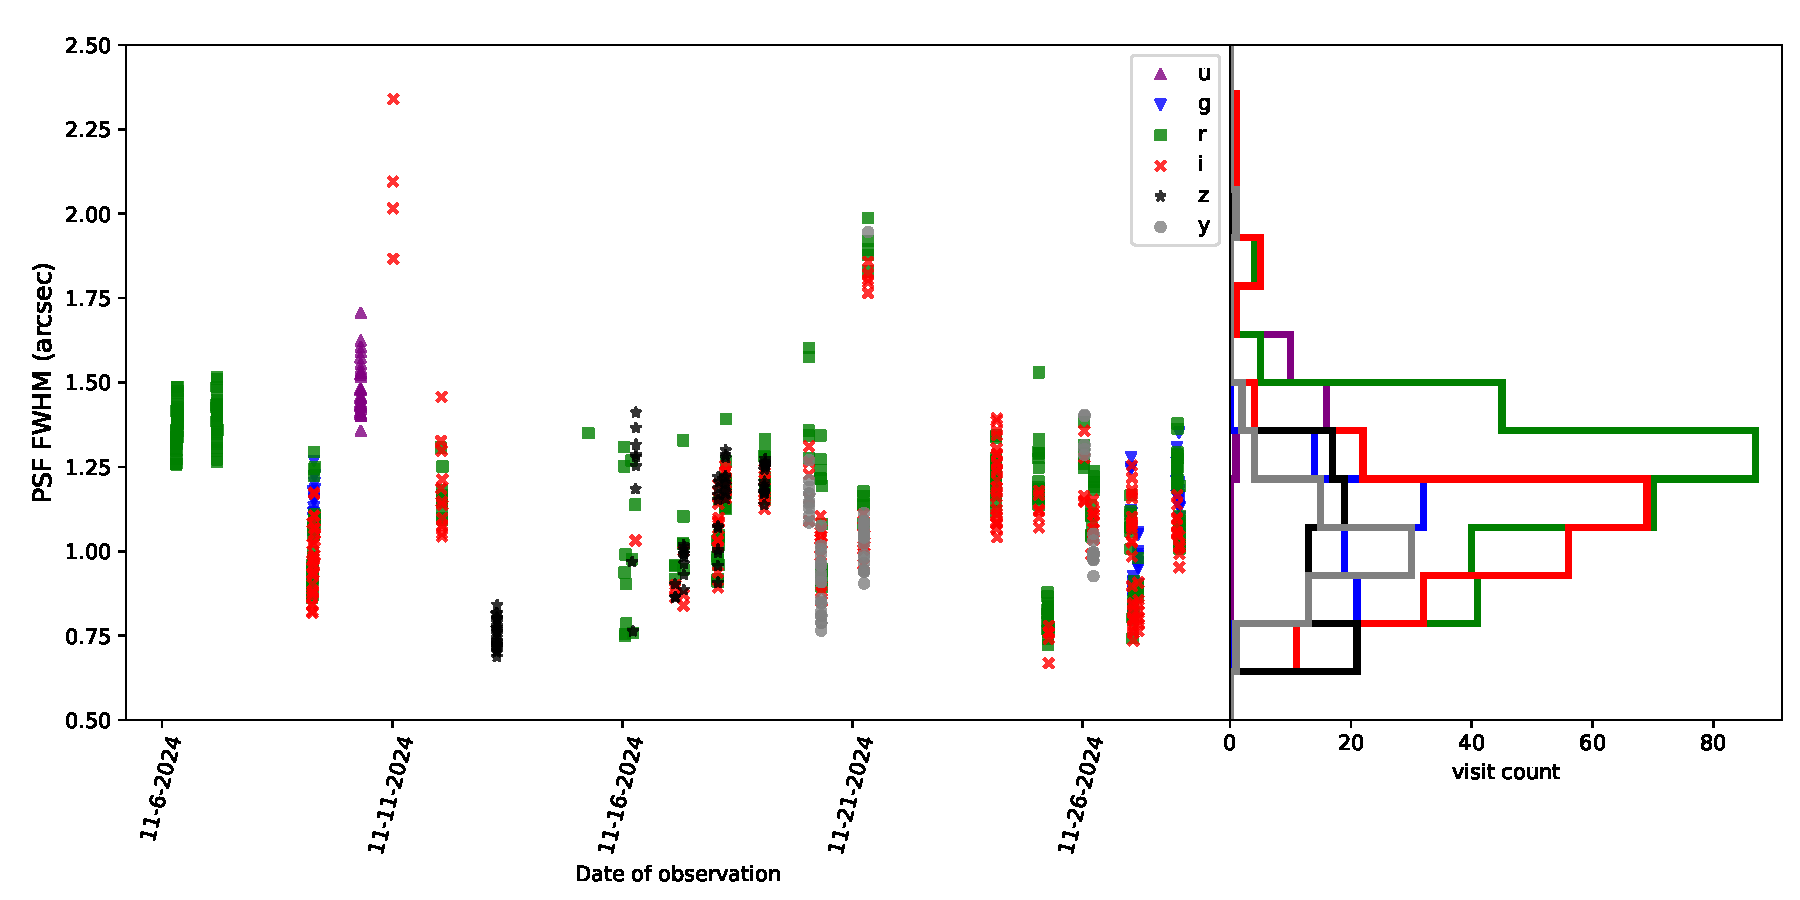
\includegraphics[width=\textwidth]{figures/seeing}
        \caption{\small PSF FWHM as a function of the observed date. Data are from DRP from 2024-11-01 to 2024-11-28.}
        \label{seeing_plot}
\end{figure*}


\begin{table*}
\centering
\begin{tabular}{@{}lccc@{}}
\textbf{Filter} & \textbf{Number of Visits} & \textbf{Mean PSF FWHM} & \textbf{STD PSF FWHM} \\ 
All           & 775                      & 1.12                   & 0.23                  \\
u             & 28                       & 1.49                   & 0.08                  \\
g             & 86                       & 1.07                   & 0.14                  \\
r             & 307                      & 1.18                   & 0.22                  \\
i             & 203                      & 1.09                   & 0.24                  \\
z             & 85                       & 1.01                   & 0.21                  \\
y             & 66                       & 1.04                   & 0.18                  \\ 
\end{tabular}
\caption{Summary of PSF FWHM statistics. Data are from DRP from 2024-11-01 to 2024-11-28.}
\label{tab:psf_summary}
\end{table*}


\subsubsection{PSF Modeling}

Two different PSF models are currently used in the DM pipeline: PSFEx, which provides a fast preliminary PSF estimation, and Piff, used later in the pipeline for more accurate PSF modeling. During the initial data collection with \ComCam and AOS testing, most in-focus star shapes exhibited doughnut-like patterns, reflecting residual optical aberrations that had not yet been corrected. This specific form of asymmetry posed challenges for PSF modeling and was not typical. Interestingly, Piff, despite being the more advanced model, struggled to handle the large, non-symmetric PSFs compared to PSFEx. Fig. \ref{growth_plot} shows how we were able early in the observation to constrain the PSF.


\begin{figure*}
        \centering
        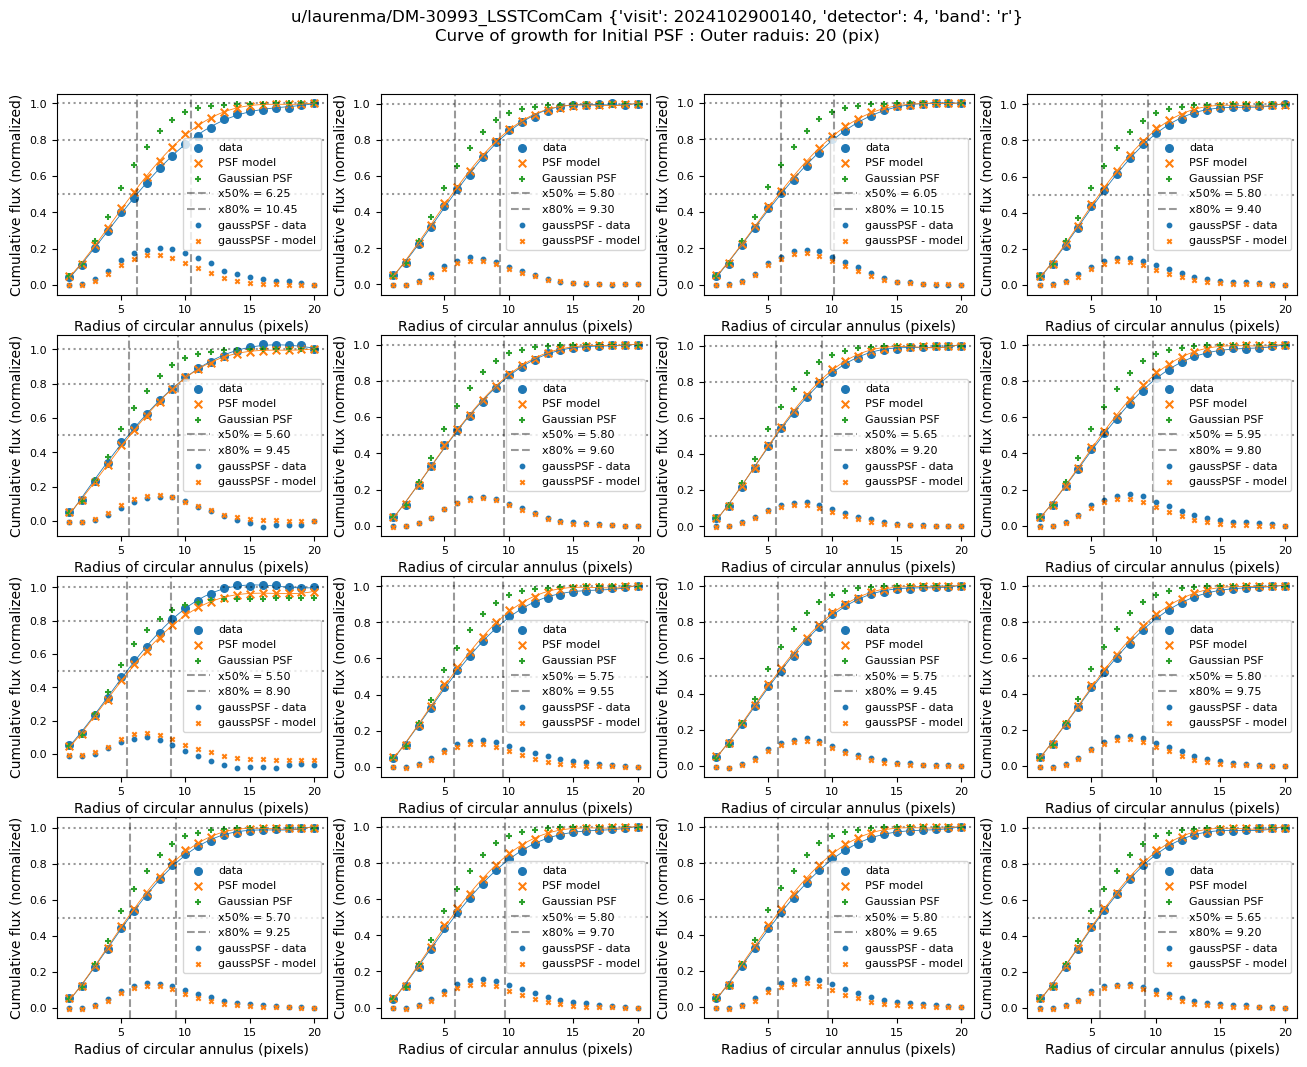
\includegraphics[scale=0.2]{figures/curveOfGrowth_pfsex_u_laurenma_DM-30993_LSSTComCam_2024102900140_4}
        \caption{\small Growth curves of the PSF compared to its model (PSFex here)  in the early data taken with \ComCam. }
        \label{growth_plot}
\end{figure*}



However, as the AOS system improved image quality and produced more symmetric PSFs, we observed behavior more consistent with expectations for both PSFEx and Piff. 
Analysis of second-moment reconstructions shows that PSFEx has a systematic offset in size reconstruction compared to Piff, which aligns with observations from DES. Overall, Piff demonstrates better PSF reconstruction, as illustrated in Fig. \ref{DT_plot}. 

\begin{figure*}
        \centering
        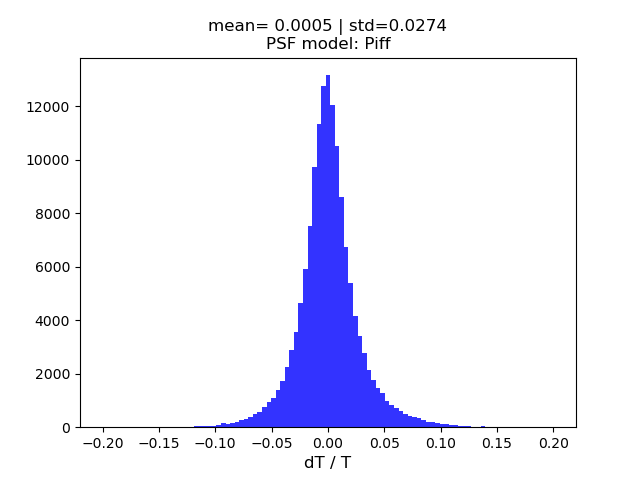
\includegraphics[scale=0.47]{figures/0_dT_1d_Piff}
        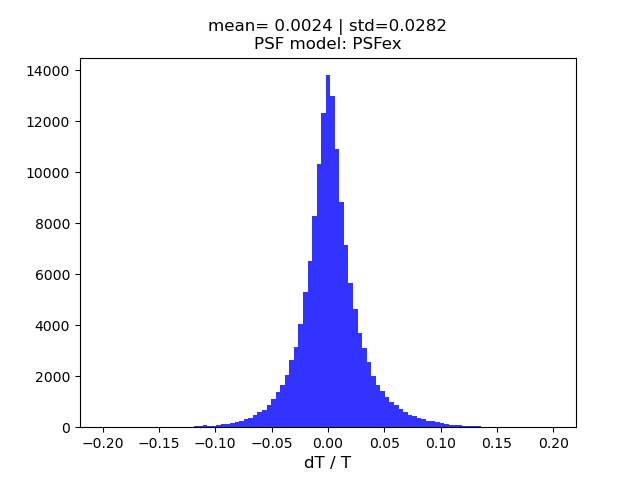
\includegraphics[scale=0.47]{figures//0_dT_1d_PSFex}
        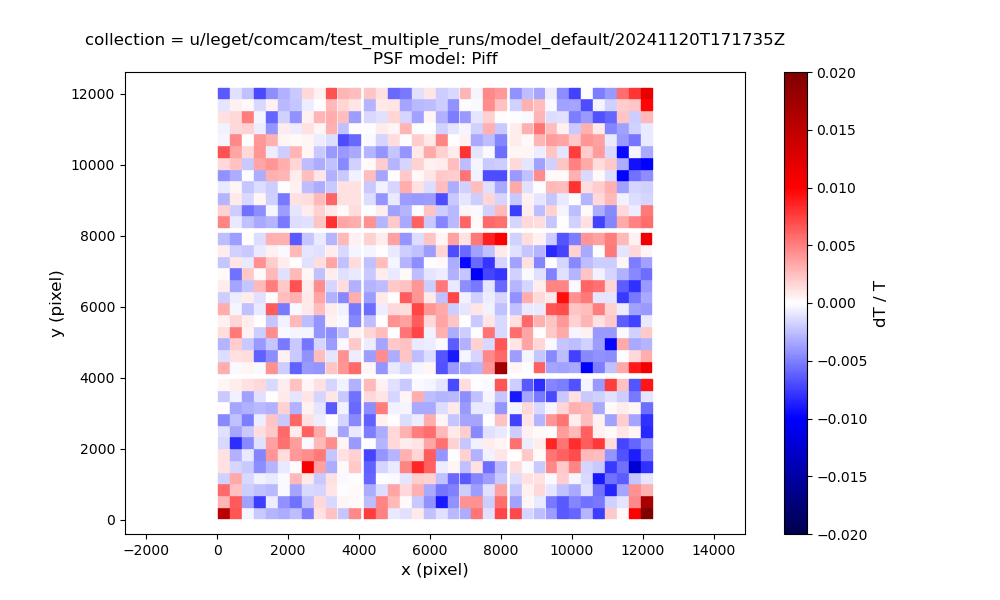
\includegraphics[scale=0.3]{figures/0_dT_2d_Piff}
	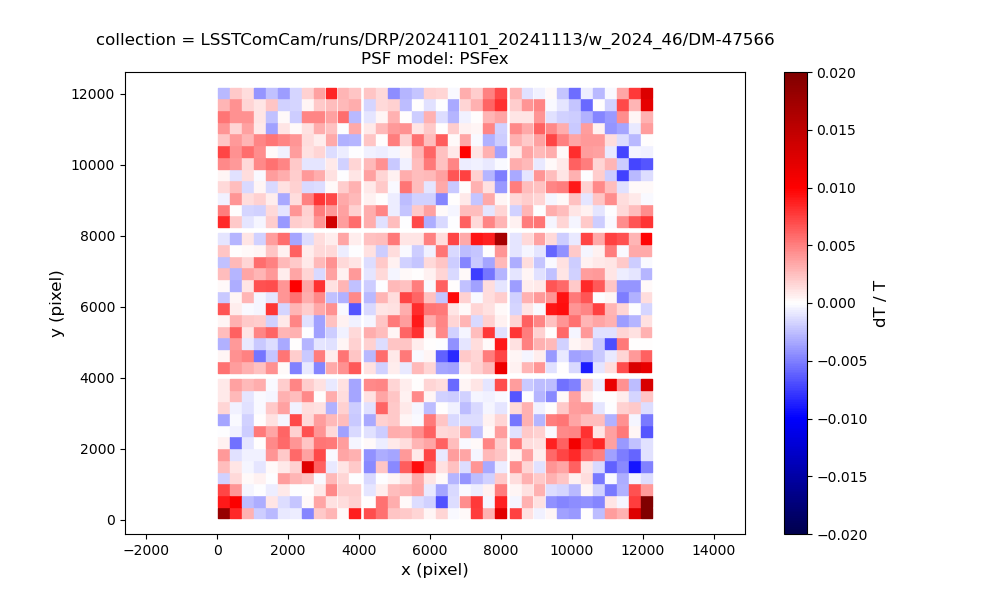
\includegraphics[scale=0.3]{figures/0_dT_2d_PSFex}
        \caption{\small Size residuals for Piff and PSFex (1d distribution and 2d average across visits). Piff has no offset and smaller scatter. Both panels 
        exhibit spatial structure across the focal plane, based on spatial averages across all science visits. The PSF is modeled per CCD in pixel coordinates 
        using a second-order polynomial for interpolation. The observed structure is unlikely to result from atmospheric or dome effects, given that this plot 
        represents an average across visits. Instead, it likely reflects spatial variations not captured by the second-order polynomial interpolation, such as 
        optical aberrations or sensor anomalies.}
        \label{DT_plot}
\end{figure*}


\subsubsection{Understanding PSF Physics}


With LSSTCam, we aim to leverage wavefront sensor data to estimate the optical system's current state and model the optical contribution to the PSF, ultimately building a physical PSF model. During AOS testing with ComCam, the optical state was estimated using out-of-focus images to predict the optical contribution to PSF shape. A ray-tracing analysis showed that the optics fitted from these images could predict the PSF shape, providing strong evidence that a physical PSF model could be developed for LSSTCam (See  Fig. \ref{PSF_plot})


\begin{figure*}
        \centering
        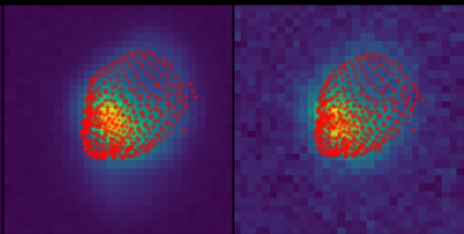
\includegraphics[scale=0.47]{figures/plot_psf_1}
        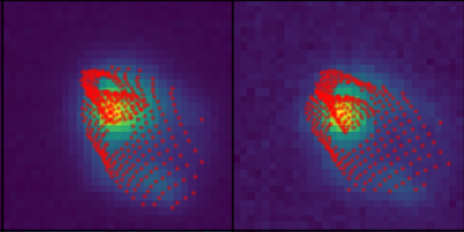
\includegraphics[scale=0.47]{figures/plot_psf_2}
        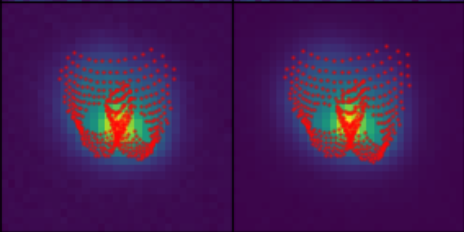
\includegraphics[scale=0.47]{figures/plot_psf_3}
        \caption{\small In-focus stars and prediction from the ray tracing on predicting PSF shape (red-dot). Optics parameters on the ray tracing side were derived from out of focus images by measuring optical aberration on "donuts" (out of focus star).}
        \label{PSF_plot}
\end{figure*}

% We’re writing a tech note (SITCOMTN-149) to capture our
% understanding of the state of the system during on-sky commissioning
% campaign with ComCam.  Please use this ticket to capture the work.
%
% From the introduction:
%
% The Vera C. Rubin Observatory on-sky commissioning campaign using
% the Commissioning Camera (ComCam) began on 24 October 2024 and is
% forecasted to continue through mid-December 2024. This interim
% report provides a concise summary of our understanding of the
% integrated system performance based tests and analyses conducted
% during the first weeks of the ComCam on-sky campaign. The emphasis
% is distilling and communicating what we have learned about the
% system. The report is organized into sections to describe major
% activities during the campaign, as well as multiple aspects of the
% demonstrated system and science performance.
%
% Charge:
%
% The groups within the Rubin Observatory project working on each of
% the activities and performance analyses are charged with
% contributing to the relevant sections of the report. The anticipated
% level of detail for the sections ranges from a paragraph up to a
% page or two of text, depending on the current state of
% understanding, with quantitative performance expressed as summary
% statistics, tables, and/or figures.  The objective for this document
% is to summarize the state of knowledge of the system, rather than
% how we got there or “lessons learned”. The sections refer to
% additional supporting documentation, e.g., analysis notebooks, other
% technotes with further detail, as needed. Given the timelines for
% commissioning various aspects of the system, it is natural that some
% sections will have more detail than others.

\subsection{Instrument Signature Removal}
\label{sec:isr}
\newcommand{\czw}[1]{
  \textbf{CZW: }\textcolor{red}{#1}
}
The quality of the instrument signal removal (ISR) has improved during commissioning, as we create and deploy updated calibration products that better represent the \ComCam system.
The following discussion summarizes our current understanding of a variety of features, both expected and newly seen on \ComCam, and presents our expected prognosis of the behavior of the full LSSTCam.

\subsubsection{Phosphorescence}

There are regions on some of the detectors (most visible in R22\_S01, detector=1) which show bright emission, particularly at bluer wavelengths, as shown in \figRef{isr_phosphorescence_example}.
This is believed to be caused by a thin layer of remnant photo-resist from the manufacturing process that remained on the detector surface, and is now permanent due to the subsequent addition of the anti-reflective coating.
In addition to the large areas, there are also discrete point-source-like or cosmic-ray-like defects caused by accumulations of this material.
Adding to the difficulty of mitigating these defects is that this photo-resist is known to be phosphorescent, explaining why these regions are more noticeable in the bluer filters.

The initial studies of this show that these features can continue to emit light up to several minutes after they've been illuminated.
Due to the long duration of these features, we decided to place manual defect masks over the worst regions.
The first of these manual masks takes up about 3.5\% of that detector, smaller than but consistent with estimates that this would create a pixel loss of approximately one amplifier.

\begin{figure}
  \begin{center}
  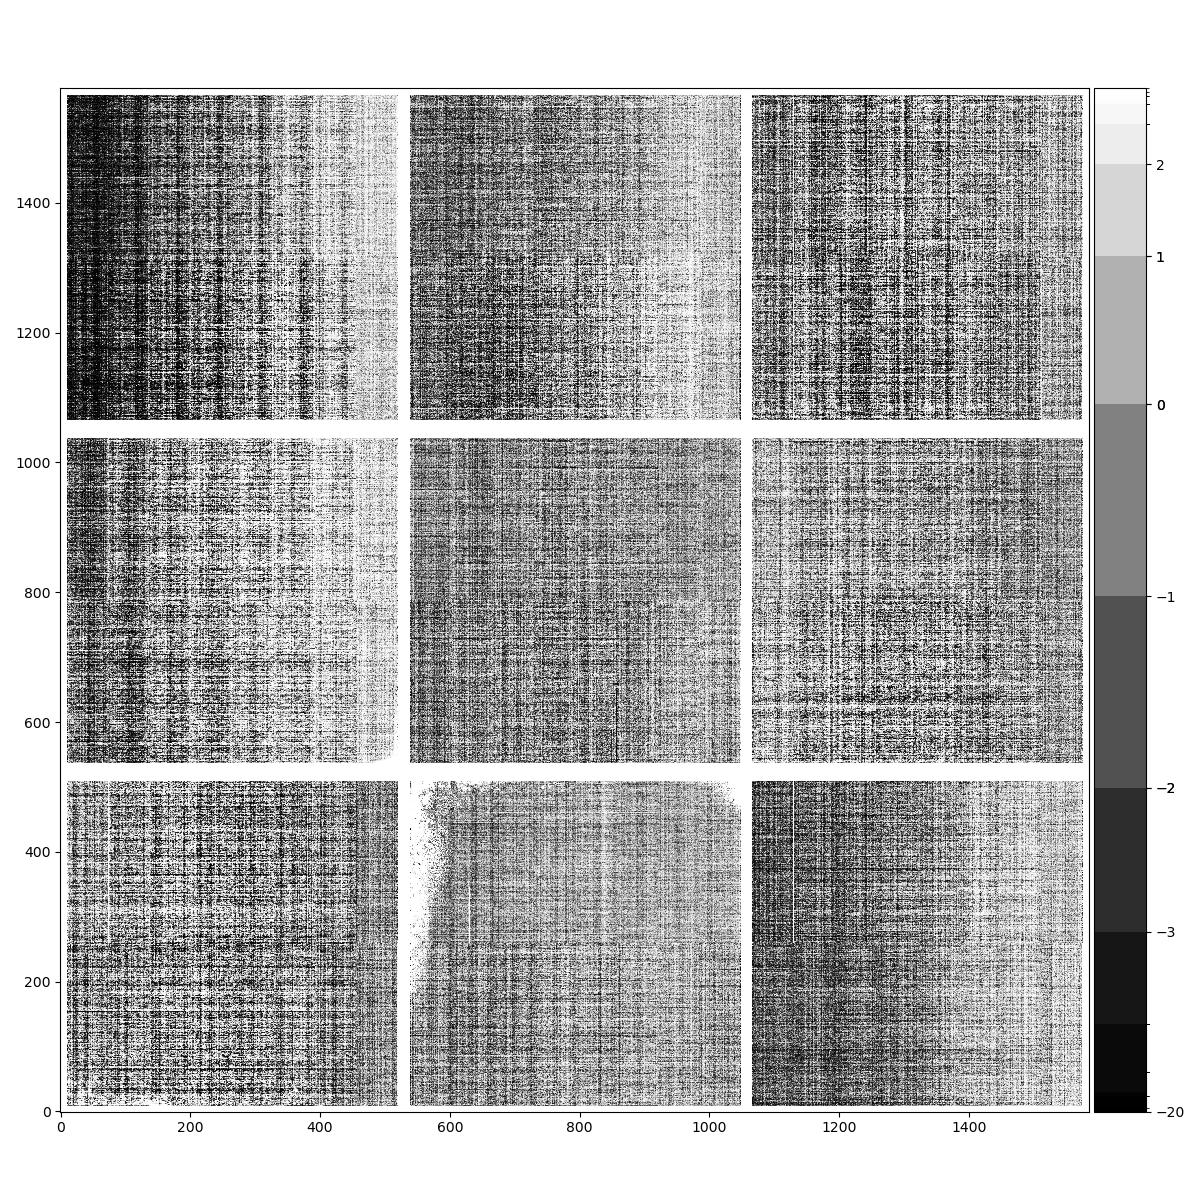
\includegraphics[width=0.5\textwidth]{figures/isr-f01-phosphor_dark_exposure.jpg}
  \caption{The phosphorescence seen in R22\_S01, shown here in a dark exposure taken after a series of twilight flats (exposure=2024112000065).  This material absorbs light at bluer wavelengths and re-emits that energy over a wide range of wavelengths.}
  \label{fig:isr_phosphorescence_example}
  \end{center}
\end{figure}

\begin{figure}
  \begin{center}
  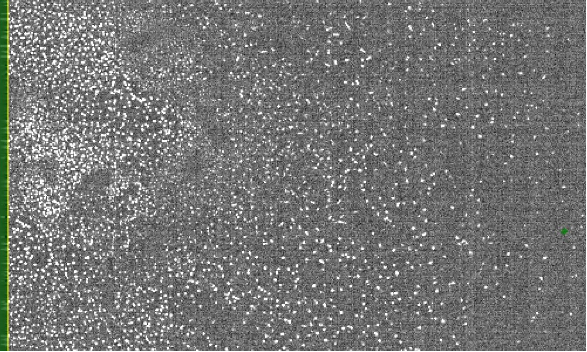
\includegraphics[width=0.8\textwidth]{figures/isr-f02-phosphorescence_point_like.pdf}
  \caption{A full-resolution view of the edge of R22\_S01.  The features shown in this image are point-like sources caused by the trapped phosphorescence photo-resist.}
  \end{center}
\end{figure}

The ITL detectors in LSSTCam are believed to have been cleaned better, so this should be less of an issue on the full camera.

\subsubsection{Vampire pixels}

There are defects on \ComCam that have been classified as ``vampire'' pixels, as they appear as a bright defect with a (generally) axisymmetric region surrounding the bright core, as if the defect is draining charge from its neighbors.
The naming is at least broadly correct, as integrating to large radii shows that these regions do appear to conserve charge.
There is an intensity dependence that makes these vampire pixels different than standard hot pixels, as these pixels do not show up on dark frames, only on flats and science exposures, where the detector surface is illuminated.
After the initial discovery of the bright obvious vampires, we added new masking code that identifies the bright cores that are above 2.0 on the combined flat (pixels that are greater than 200\% of the median flat level), and adds circular masks to the defect list.
This appears to find the most problematic examples, but as we have improved flat quality during commissioning, we are finding that there is a sub-population that are not as severe, but likely have a similar physical mechanism.
This population is still bright on the flat, with peaks around 1.2 (20\% elevated relative to the flat), and may need to be masked as well.
From an initial study in the lab, it appears that all ITL detectors on LSSTCam have a few of these kinds of defects, with two detectors approaching similar contamination levels as R22\_S10 on \ComCam.

\begin{figure}
  \begin{center}
  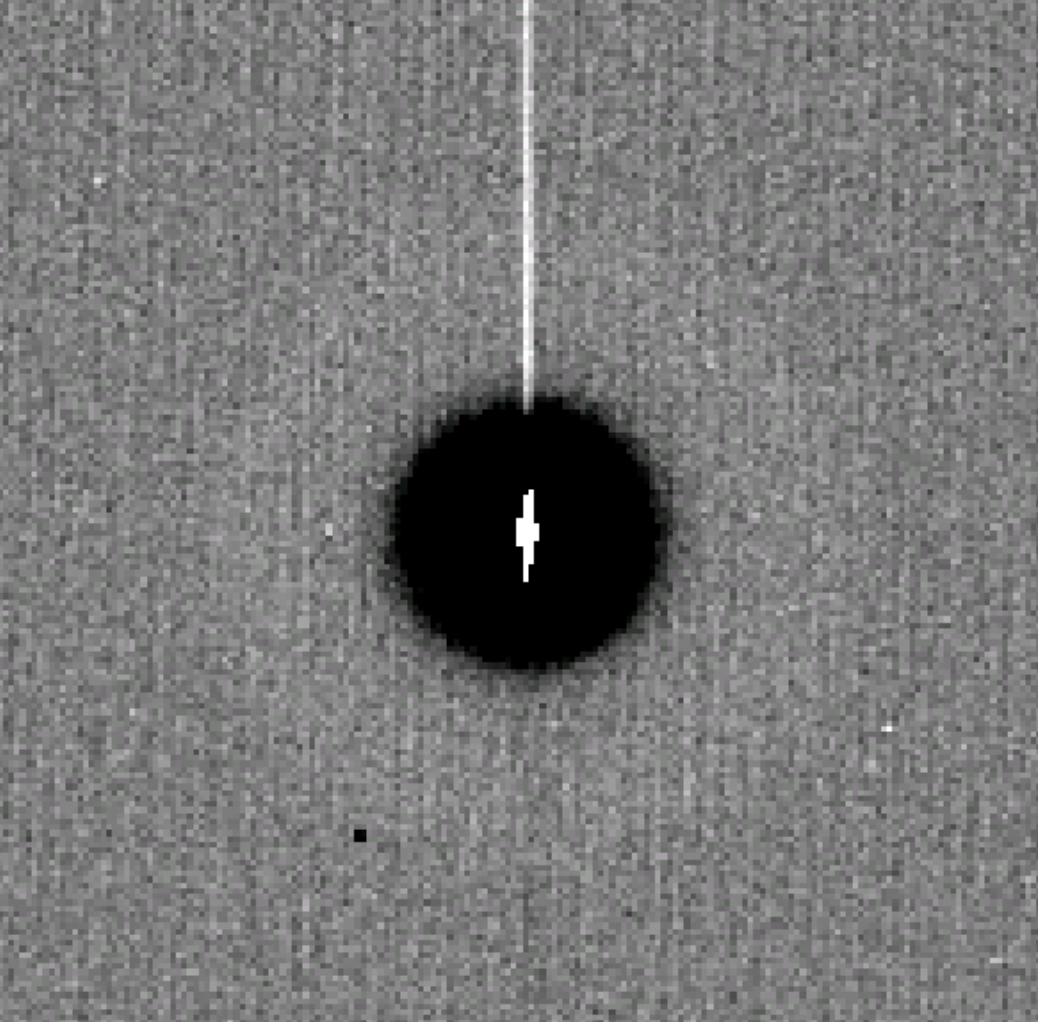
\includegraphics[width=0.5\textwidth]{figures/isr-f03-vampire_pixel.png}
  \caption{A close up of one of the largest vampire pixels.  The bright core and region of depletion are clearly visible.  Currently we only mask the core and depleted region, but will be extending this to mask the persistence-like trail that this feature leaves in the next few weeks.}
  \end{center}
\end{figure}

\begin{figure}
  \begin{center}
  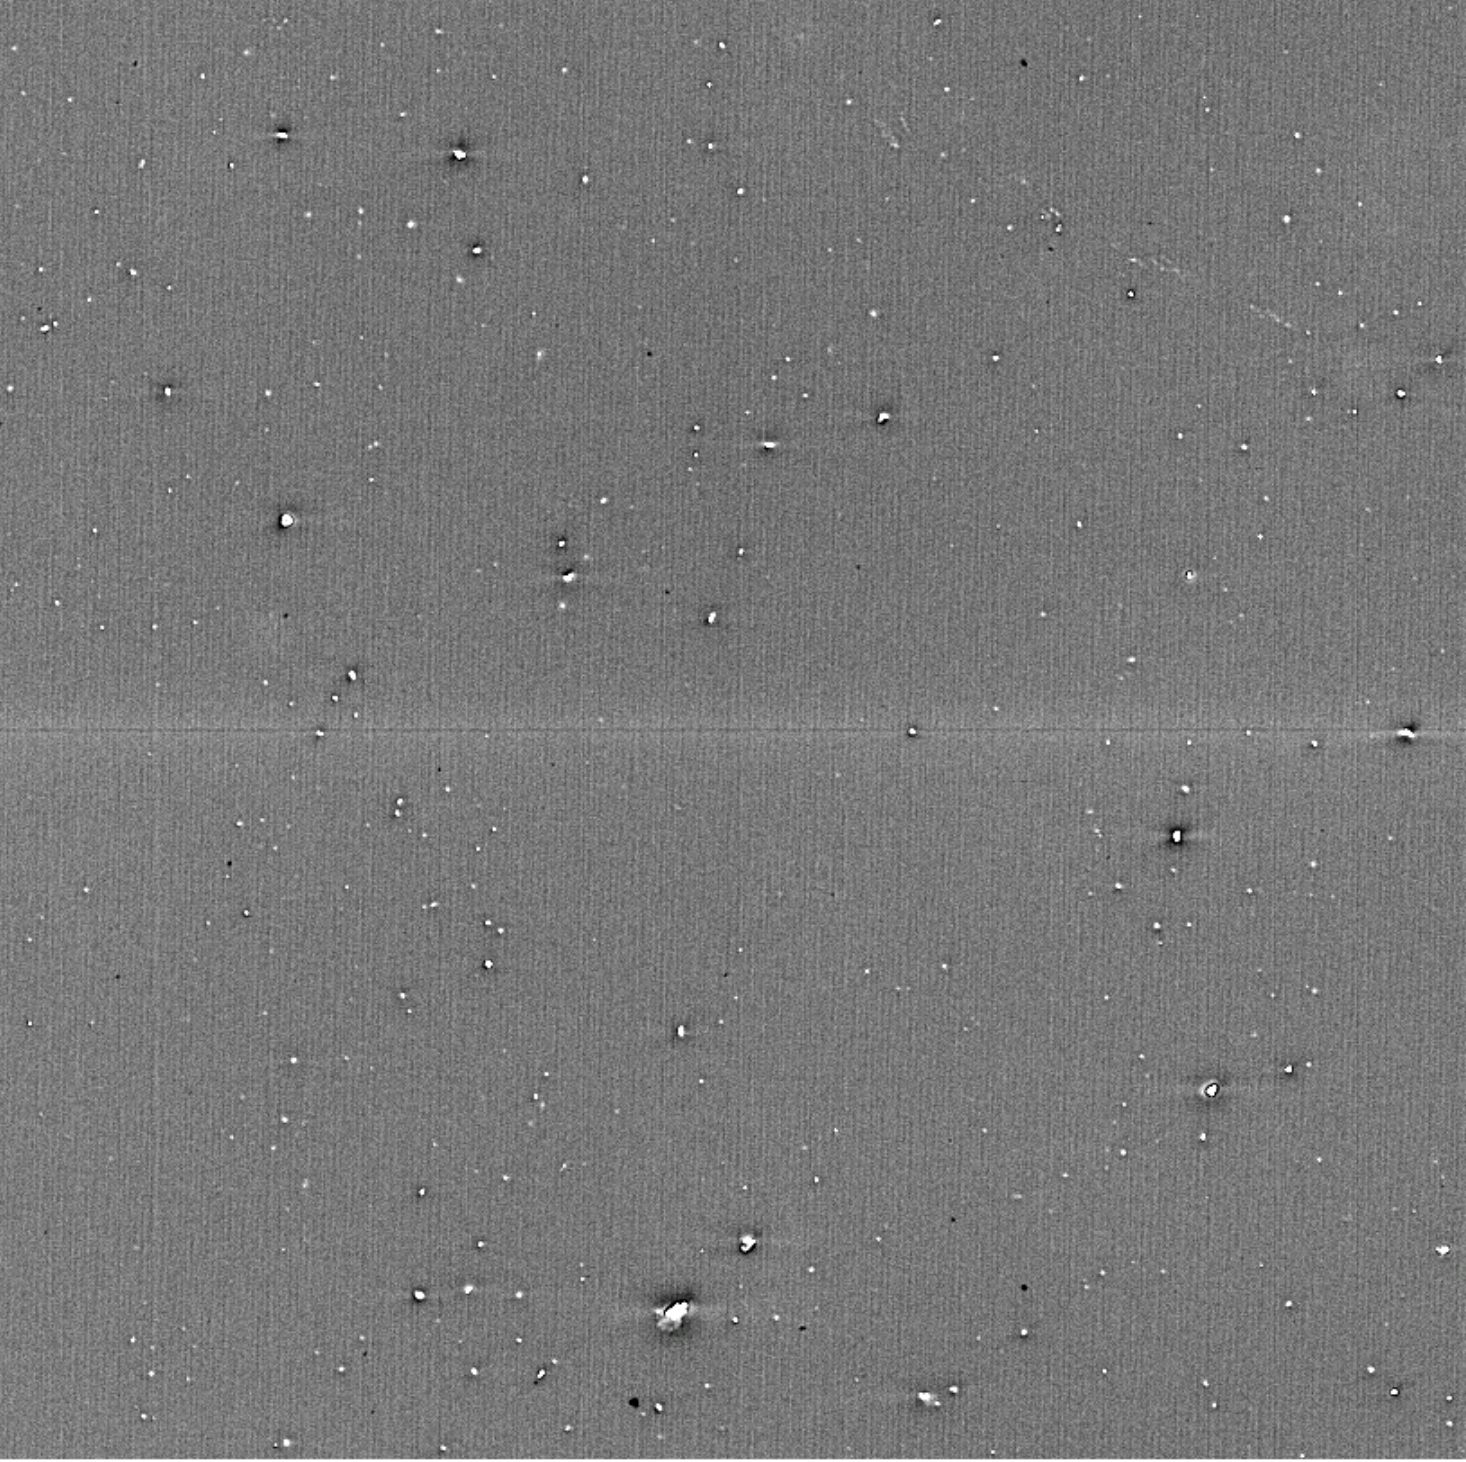
\includegraphics[width=0.5\textwidth]{figures/isr-f04-vampire_pixels_y_det03.png}
  \caption{A view of detector R22\_S10 in y-band, which has a large number of less significant vampire pixels.}
  \end{center}
\end{figure}


\subsubsection{Saturated star effects}

\begin{figure}
  \begin{center}
\linkedFigure{https://rubin-obs.slack.com/files/U0772GZSR8W/F081SU3FAE6/19zqa.png?origin_team=T02SVMGU4&origin_channel=C07RV29CXSR}
    \caption{
      A portion of \texttt{day\_obs 20241127 seq\_num 488} showing the vertical bands which are apparently
        produced by very bright (saturated?) pixels.
    }
\label{fig:darkStreaks}
  \end{center}
\end{figure}

Although we expected to find saturated star trails coming from bright sources, the observed behavior of these trails is unique.
Saturation spikes on most cameras appear as streaks extending from the core of the bright source along the
direction of the parallel transfers, and truncate as the charge bleeds run out of charge (and can no longer
overcome the potentials defining the pixel).
The trails seem with \ComCam, however, extend the entire height of the detectors, crossing the midline break
(as is to be expected in the ITL, but not the E2V, CCDs).
These trails are also not at the expected high state, with the centers of these trails having flux levels
lower than the average sky levels, creating dark trails (See \figRef{darkStreaks}),
On the worst saturated objects, there is also evidence of charge pile-up near the serial register, which can then create fan-like bright features at the edge of the detector.
Those bright features can also then crosstalk onto other amplifiers.

The underlying physics is not well understood. The leading theory is that photo-electrons entering the
$n$-doped channel stops partially cancel the effects of the holes, leading to electric fields which
produce an effect similar to Brighter-Fatter, visible in the background level as well as in objects.
Further study is needed to see if we can correct these trails outside of the regions of charge buildup.
Until we have a correction, we plan to begin masking both the trail and the fan-spread near the serial register.

Although we haven't seen identical features on LATISS (possibly due to the much lower sky levels), the presence of these odd trails on all \ComCam detectors suggests that this is a property of the ITL devices, and so will likely be seen on LSSTCam as well.

\subsubsection{Gain ratios}

\ComCam has been the first large-scale application of the updated ``IsrTaskLSST'' task, which uses a model of how the various signals combine to form the raw images to inform how we correct those signals during the ISR process.
One improvement of this new task is that we now apply per-amplifier gains before flat correction, removing the gain component that was previously included in the flat correction.
This results in the flat containing mainly QE and illumination patterns, which is much ``flatter'' than flats that also include gain terms (which offset the amplifiers relative to each other).


If we have properly diagonalized the flats and the gains, we would expect that applying the gain correction would create images with consistent sky levels across different amplifiers.
However, when we look at images taken on-sky, our initial gain values result in some amplifiers being
significantly different than their neighbors (\figRef{raft_flat_ratio}).
The gains that we use are derived from the photon transfer curve (PTC), which uses flat pairs at different flux levels to monitor the properties of the noise.
We have two of these sequences taken in the lab, and they disagree at the few percent level.
This is similar in scale to the errors necessary to explain the on-sky differences.
Further complicating this issue, the offsets seen in twilight data (used for flats) and that seen during the
night also seem to differ (\figRef{amp_gain_ratios})
These differences so far have not been found to correlate with any device temperature, time, or voltage values.
The gain correction fix appears to be stable, as we've only needed to generate and apply it once.

\begin{figure}
  \begin{center}
  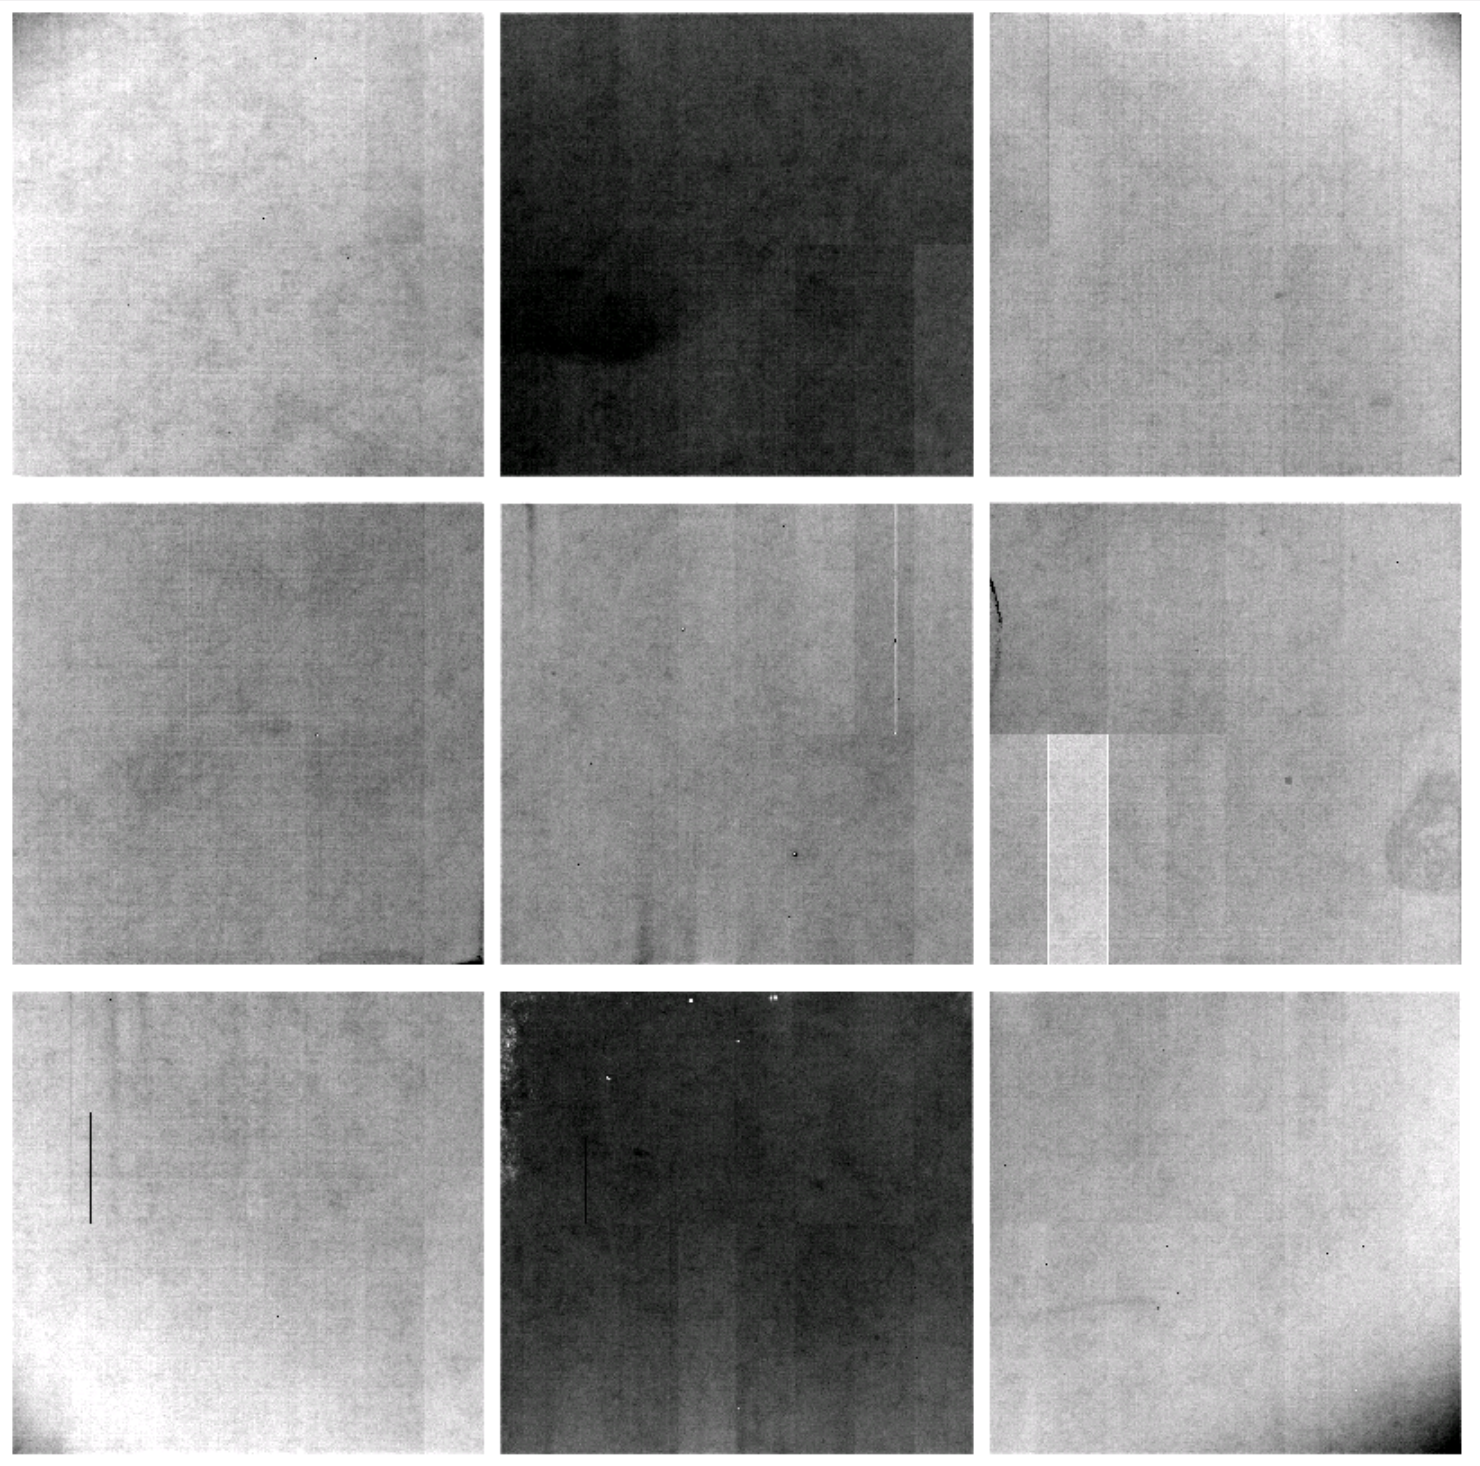
\includegraphics[width=0.5\textwidth]{figures/isr-f06-twilight_flat_ratio.png}
  \caption{The ratio of the twilight-flat divided by a flat constructed from 94 r-band science frames.  The
    scaling ranges from 0.9905 to 1.007.  The visibility of amplifiers is caused by the unknown gain errors.
    The bottom right corner amplifier (C07) on R22\_S21 is one of the indicator amplifiers, as it diverges
    from its neighbors.  Although the C00-C03 amplifiers in R22\_S12 also show significant offsets, these
    amplifiers also have an unrelated CTI issue, making them less reliable indicators.}
  \label{fig:raft_flat_ratio}
  \end{center}
\end{figure}

\begin{figure}
  \begin{center}
  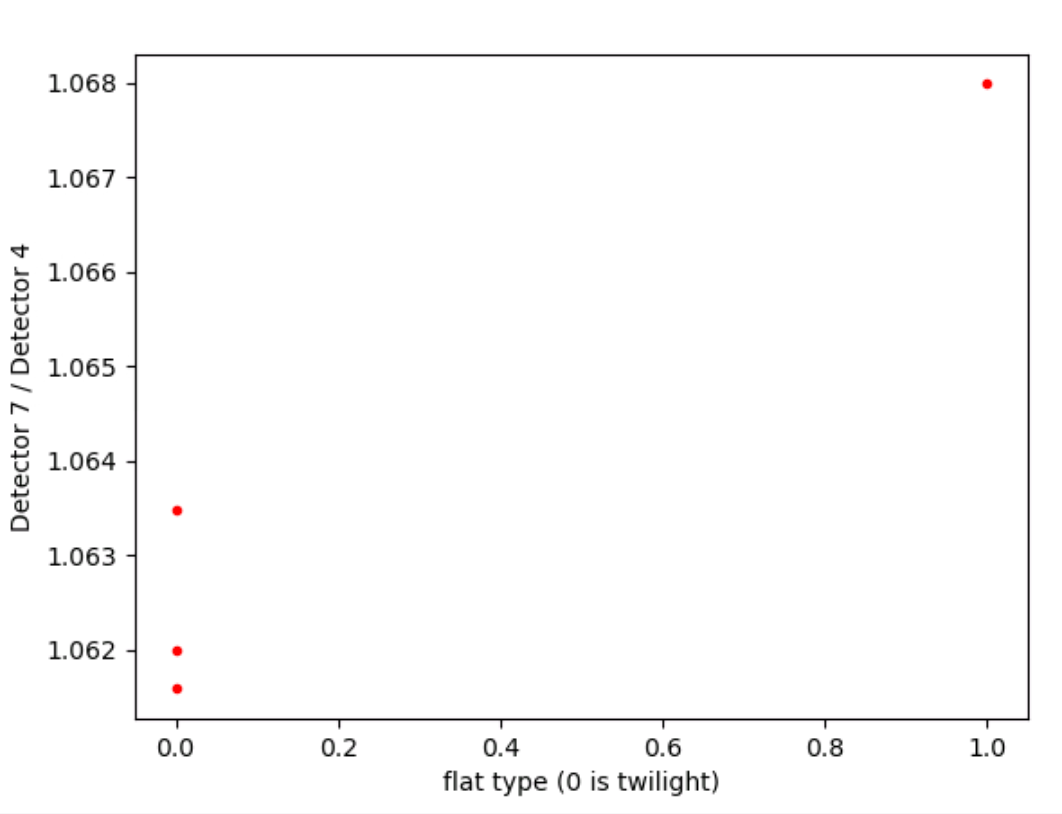
\includegraphics[width=0.5\textwidth]{figures/isr-f05-gain_ratios_by_flat.png}
  \caption{A comparison of the gain ratio between amplifiers in R22\_S12.  C07 is chosen as the indicator amplifier, and C04 is the reference.  We have three twilight flat measurements taken at different rotator angles, and one from the 94 input sky flat.}
  \label{fig:amp_gain_ratios}
  \end{center}
\end{figure}

\subsubsection{Crosstalk}

We are currently using crosstalk values that were constructed by averaging the lab-based ITL measurements taken on LSSTCam.
These are working better than expected, with residuals post correction being only a few electrons peak to peak.
We plan to do a more complete crosstalk study using on-sky data, but the current results suggest that these lab measurements are sufficient for \ComCam, and expect the same to be true for LSSTCam.

\subsubsection{Twilight flats}

Because the flat field screen and illuminator was not available while ComCam was on the telescope, we used dithered, tracked twilight flats to generate the combined flat calibration frames. The exposure time of the twilight flats were dynamically adjusted to hit a target count, generally in the range of 10-20k. The flats taken at a wide range of azimuth angles and rotator angles. See \figRef{twilight_counts} for the counts per pixel per second as a function of sun elevation angle.

This reduction of non-sky signals is imperfect, and an early i-band flat showed a satellite trail as a
result; this was remedied with a more recent flat built using a larger number of exposures.


\begin{figure}
  \centering
  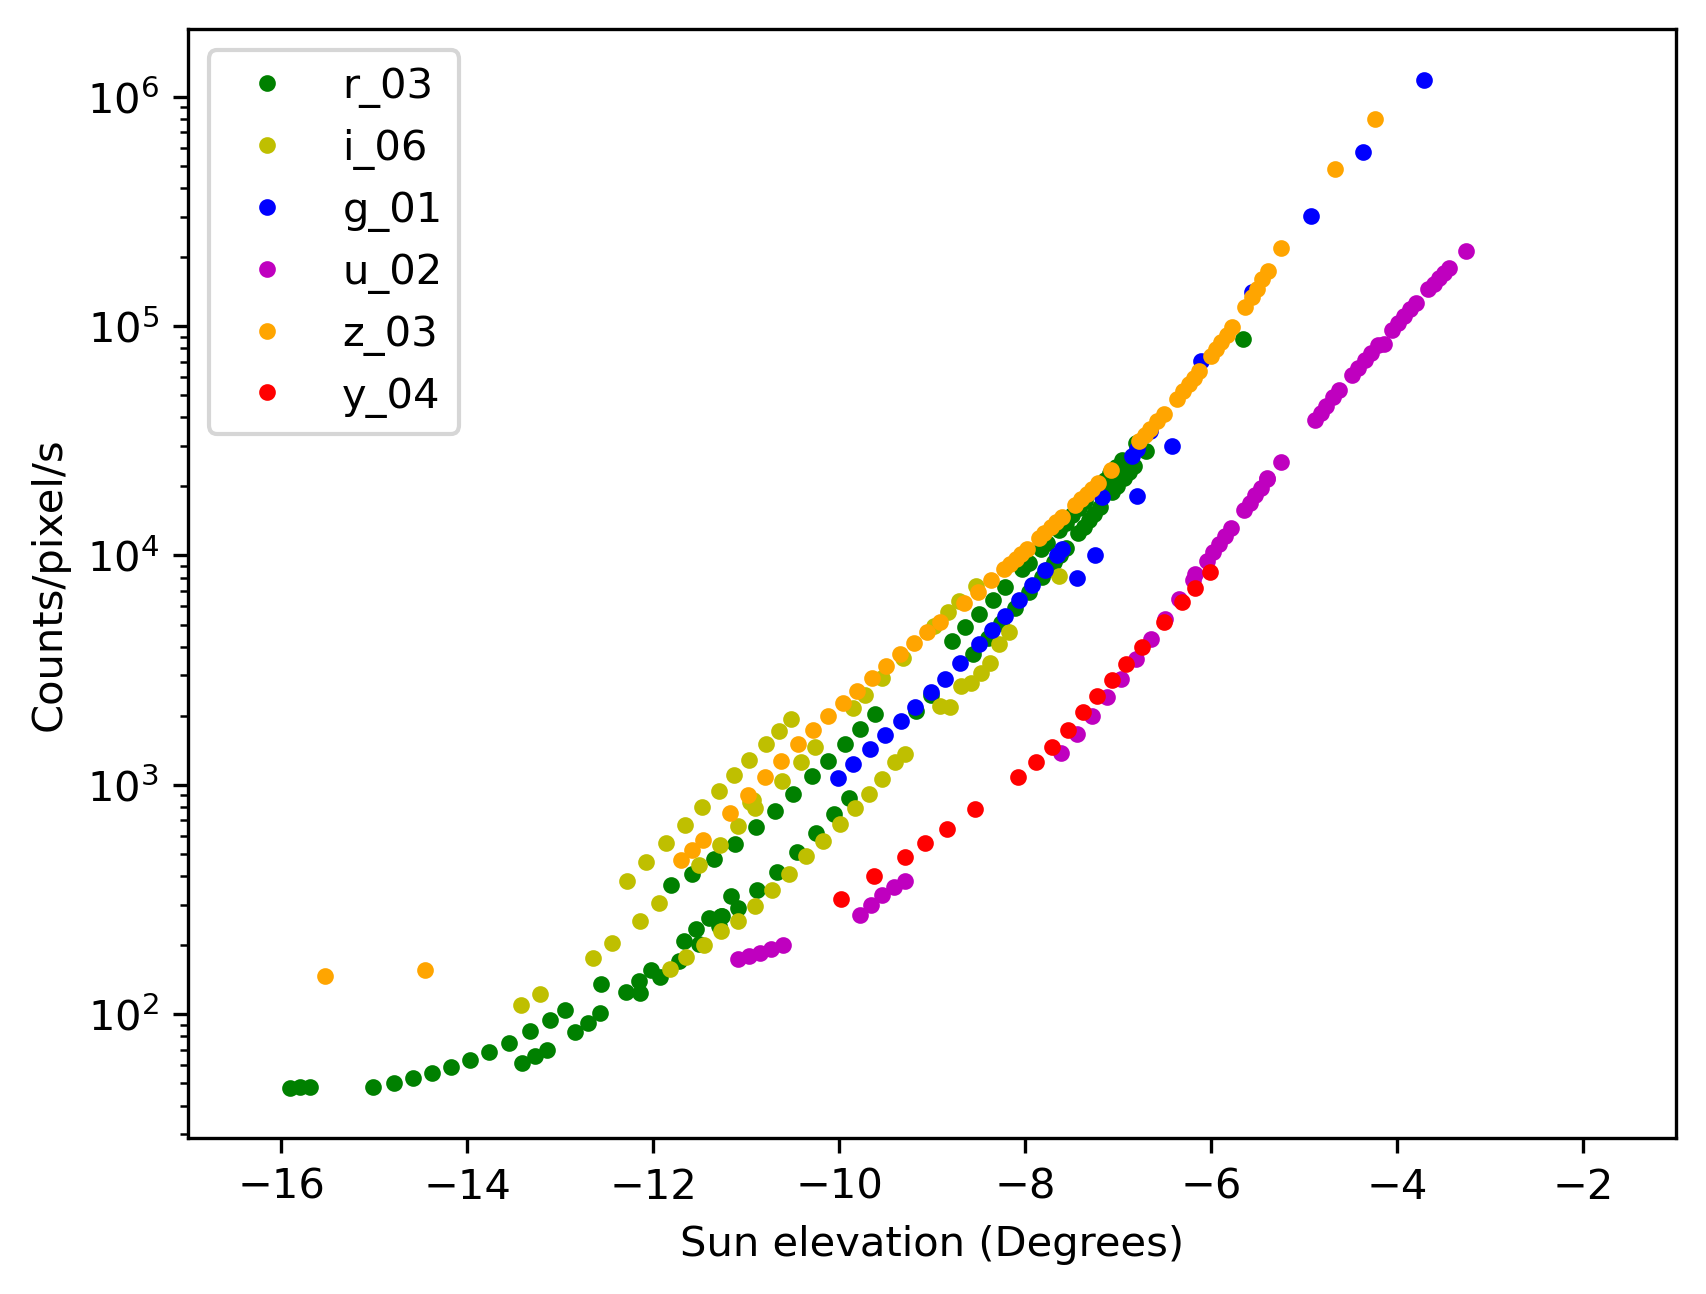
\includegraphics[width=0.5\textwidth]{calibration_data_figures/twilight_flat_counts.png}
  \caption{Twilight flat counts per pixel per second for each filter as a function of sun elevation angle.}
  \label{fig:twilight_counts}
\end{figure}

\subsubsection{Operations}

The Telescope and Auxiliary Instrumentation Calibration Acceptance Board (TAXICAB) has been meeting previously to discuss LATISS calibrations, and has been helping manage calibrations for \ComCam.
This process has not prevented problematic calibrations from being deployed (like the i-band flat with the satellite trail), but it has ensured that multiple people have checked some set of results.
We are generating calibration verification reports regularly as part of this process (available at \url{https://s3df.slac.stanford.edu/people/czw/cpv_reports/}), and plan to add new metrics and checks to these as we discover more features of these detectors.


\section{Low Surface Brightness Sources and Scattered Light}
\label{sec:low_surface_brightness}

The low-surface-brightness science team has been actively involved in investigating the \ComCam imaging. Efforts in this area have largely broken down along two avenues.

\noindent {\bf Visual Inspection:} Several members of the team have been actively engaged in image inspection with a specific eye on low-surface-brightness features. Several items that have arisen during this inspection. 

\begin{itemize}
\item {\bf Ghosts:} Ghosting, internal reflections of the light from astronomical objects off of multiple reflecting surfaces within the camera (e.g., the detectors, lenses, and filter), is a well known contaminant for low-surface-brightness science. Ghosts were first identified in images taken on the first night of \ComCam observing. Ghost patterns were associated to stars both on, and slightly off, the \ComCam field-of-view. Analysis from the batoid ray tracing code could qualitatively reproduce the ghost patterns (see below for more details).

\item {\bf Baffling:} A prominent stray light feature was noticed as concentric circles of varying intensity often situated in the corner of the \ComCam field of view. Initial incidences of this stray light were traced back to a light on the dome crane (see below); however, this pattern continues to be seen on subsequent nights.   Members of the camera crew note that there is no baffle system installed upstream of the \ComCam optics, and we expect stray light to be much reduced with LSSTCam.

\item {\bf Dome Lights:} Several lights inside and around the dome have been identified and mitigated (one particularly impactful light source was on . Pinhole images are a valuable tool for identifying these light sources, and several were identified in recent pinhole imaging. As operations becomes more routine, it is expected that the incidence of artificial light in the dome will decrease.

\item {\bf Sky over-subtraction:} Correct subtraction of the sky background around large, bright astronomical
  objects (e.g., nearby galaxies, nebulae, galaxy clusters, etc.) while making accurate measurements for faint
  objects in the frame is a challenging task. The LSB group has been tracking instances of astronomical objects that have been observed by \ComCam and are likely to suffer from background subtraction issues.

\item {\bf Artificial Satellites:} The low-surface-brightness, out-of-focus tails of bright artificial satellites may contribute structured low-surface-brightness features in stacks and coadds. While the topic of artificial satellites is largely covered in Section~\ref{sec:dia_transient_variable}, the LSB group is interested in tracking particularly prominent examples.

\end{itemize}

The group is tracking visually identified instances of many of these features in \ComCam imaging.

\noindent {\bf Quantitative Ghost Investigation:}  The `batoid` ray tracing toolkit has the ability to predict the locations and relative intensities of these ghosts. Based on early qualitative comparisons, batoid appears to be doing a good job at predicting the patterns of ghosts observed in \ComCam imaging for stars located both on and slightly off the focal plane. A more quantitative evaluation between batoid and the \ComCam imaging is now being developed to assess the precision and accuracy of the batoid model when it comes to predicting the location, morphology, and intensity of ghosts. Gaia is being used to identify bright stars that should contribute prominent ghosts. These stars are fed into batoid and the output ghost patterns are scaled by the flux of each input star as measured by Gaia. Circular templates for the ghosts are being generated by running batoid on each scattering surface individually and applying Canny edge detection and a circular Hough transform to determine to position and size of each ghost. These circular ghost templates will be compared to the observed data, and eventually fit to the intensity of the observed ghosts to verify/refine the reflectivity coefficients that batoid uses for each camera surface. While the ghosting in LSSTCam will be different from that in \ComCam, the tools developed for this analysis should be generalizable.

\noindent {\bf Future Endeavors}

The team hopes to have the chance to collect and investigated on- and off-axis dithered bright star exposures to further quantify ghosting and scattered light. The team is actively investigating metrics to characterize the variance in the sky background modeling. The team is investigating sky background fitting techniques developed on DECam. DECam calibrations have been acquired and testing of these algorithms on DECam data processed with the LSST Science Pipelines is being developed. We hope to apply the quantitative LSB tools being developed on precursor data to the \ComCam data.


This is a quick update on astrometry quality based on data collected halfway through the \ComCam observations. It is important to note that so far only single frame astrometric calibration is being done. Doing the additional global astrometric calibration with GBDES will further improve the results presented here.


For now, metrics like AM1 (the RMS of distances between star pairs separated by 5’ across all visits on a tract) appear to be satisfactory. On average, the median value across different filters is around 10 mas, as shown in Figure \ref{AM1_plot}.

\begin{figure*}
        \centering
        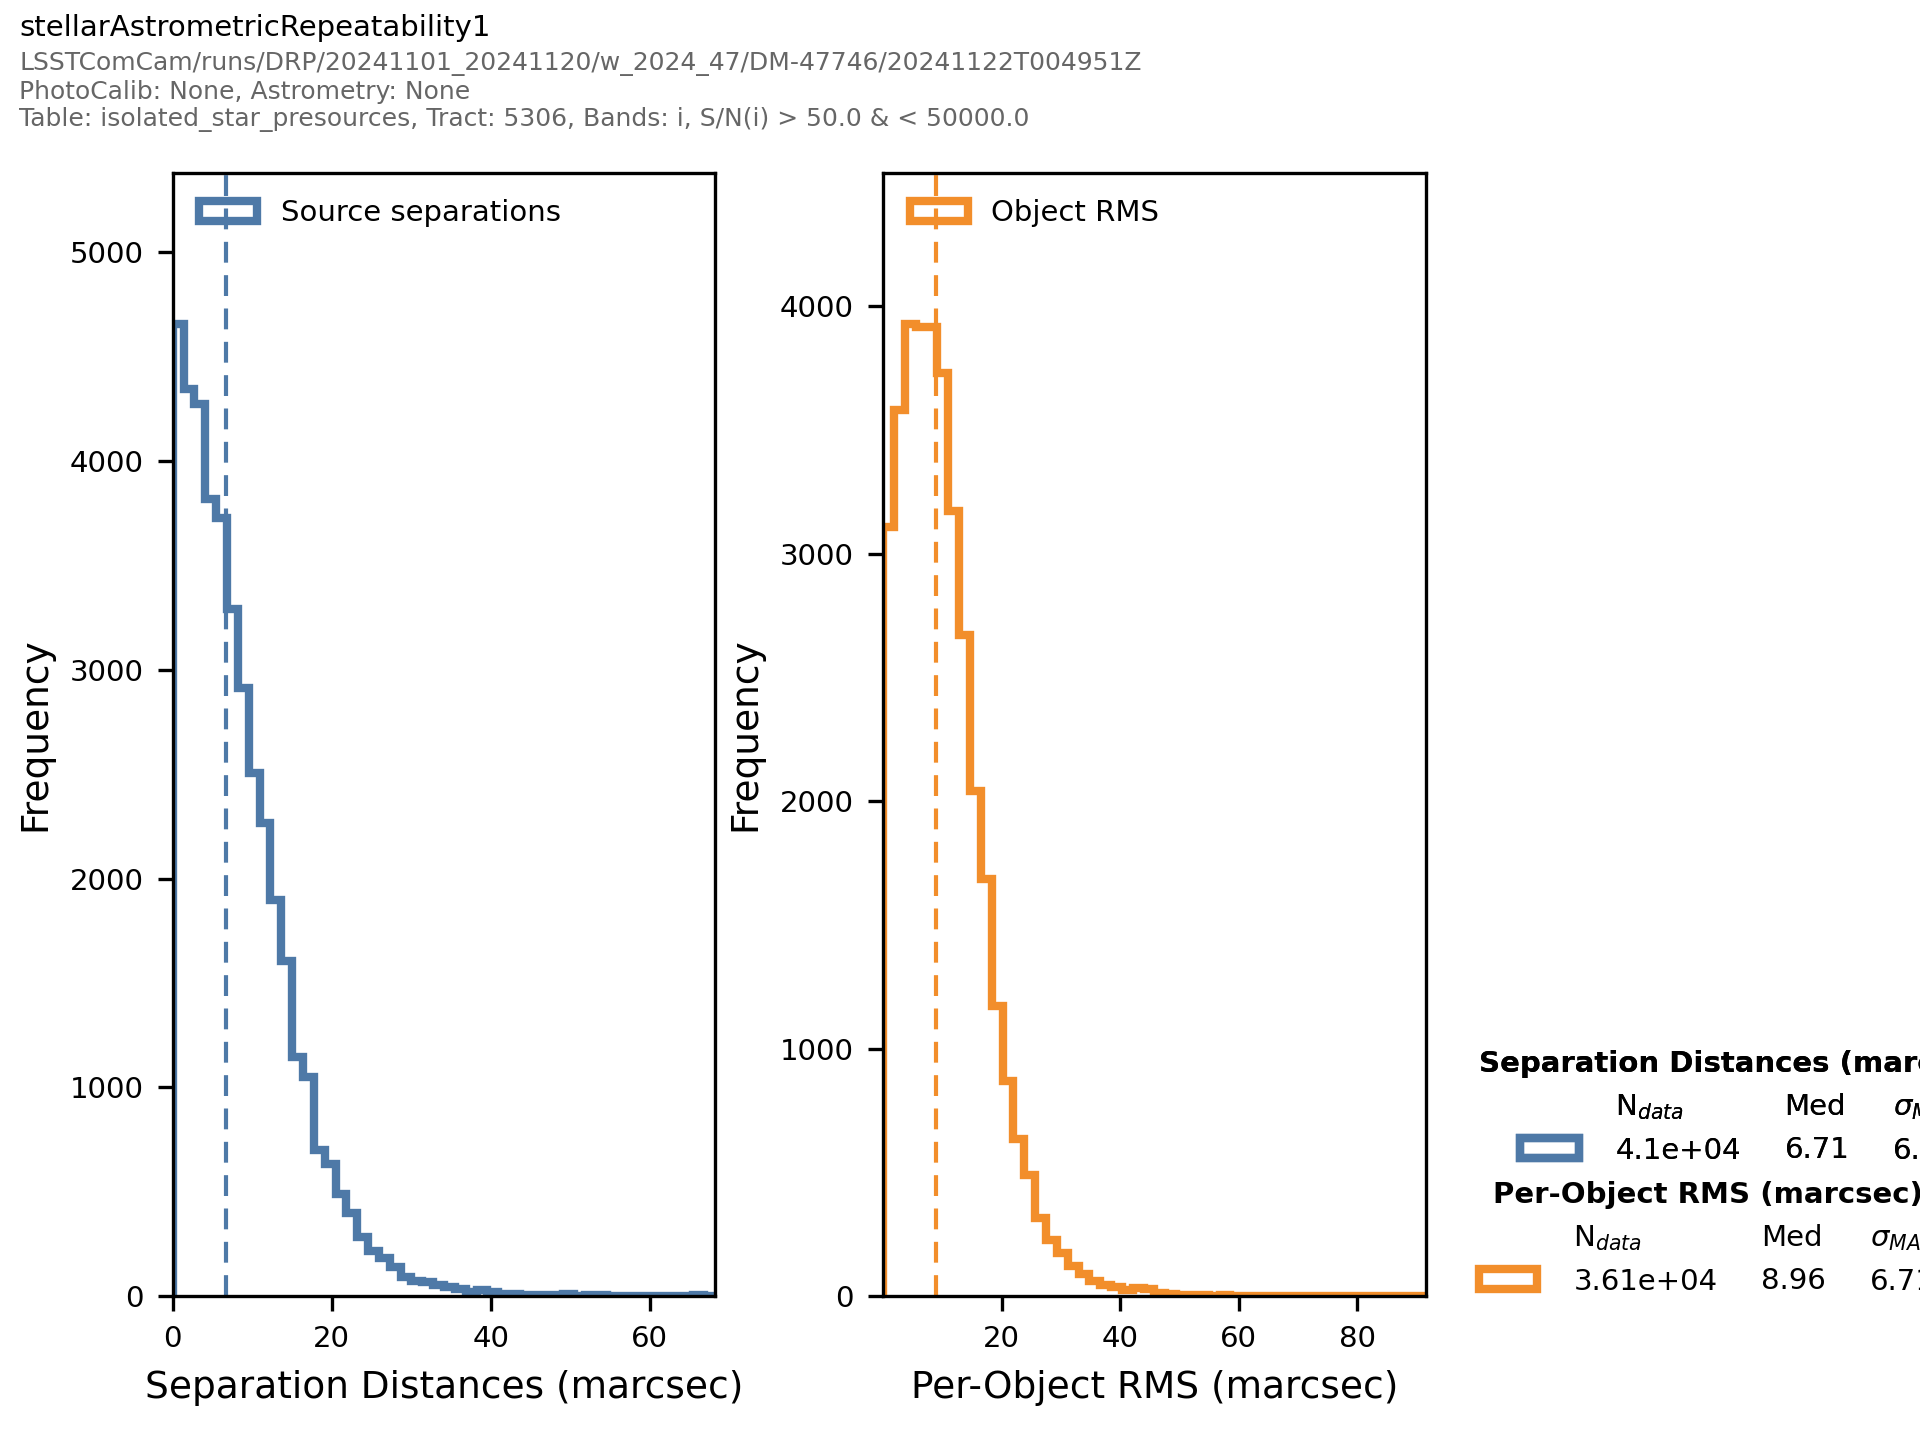
\includegraphics[scale=0.47]{figures/11d0c9f8-45f6-4bf2-871a-56e00e62060c}
        \caption{\small Stellar Astrometric repeatability in filter I in a given tract. AM1, which is the median of the orange histogram,  is below 10 mas.}
        \label{AM1_plot}
\end{figure*}

When examining the average astrometric residuals projected across the focal plane, some structures appear to be present, as in the example below in Fig \ref{fov_astrometry_plot}. However, more data is needed to confirm whether these patterns are noise or systematic effects. It is likely that GBDES will help address these structures once it is activated. Personally, I don’t think this could be noise, but it’s fine to be noncommittal about causes here.

\begin{figure*}
        \centering
        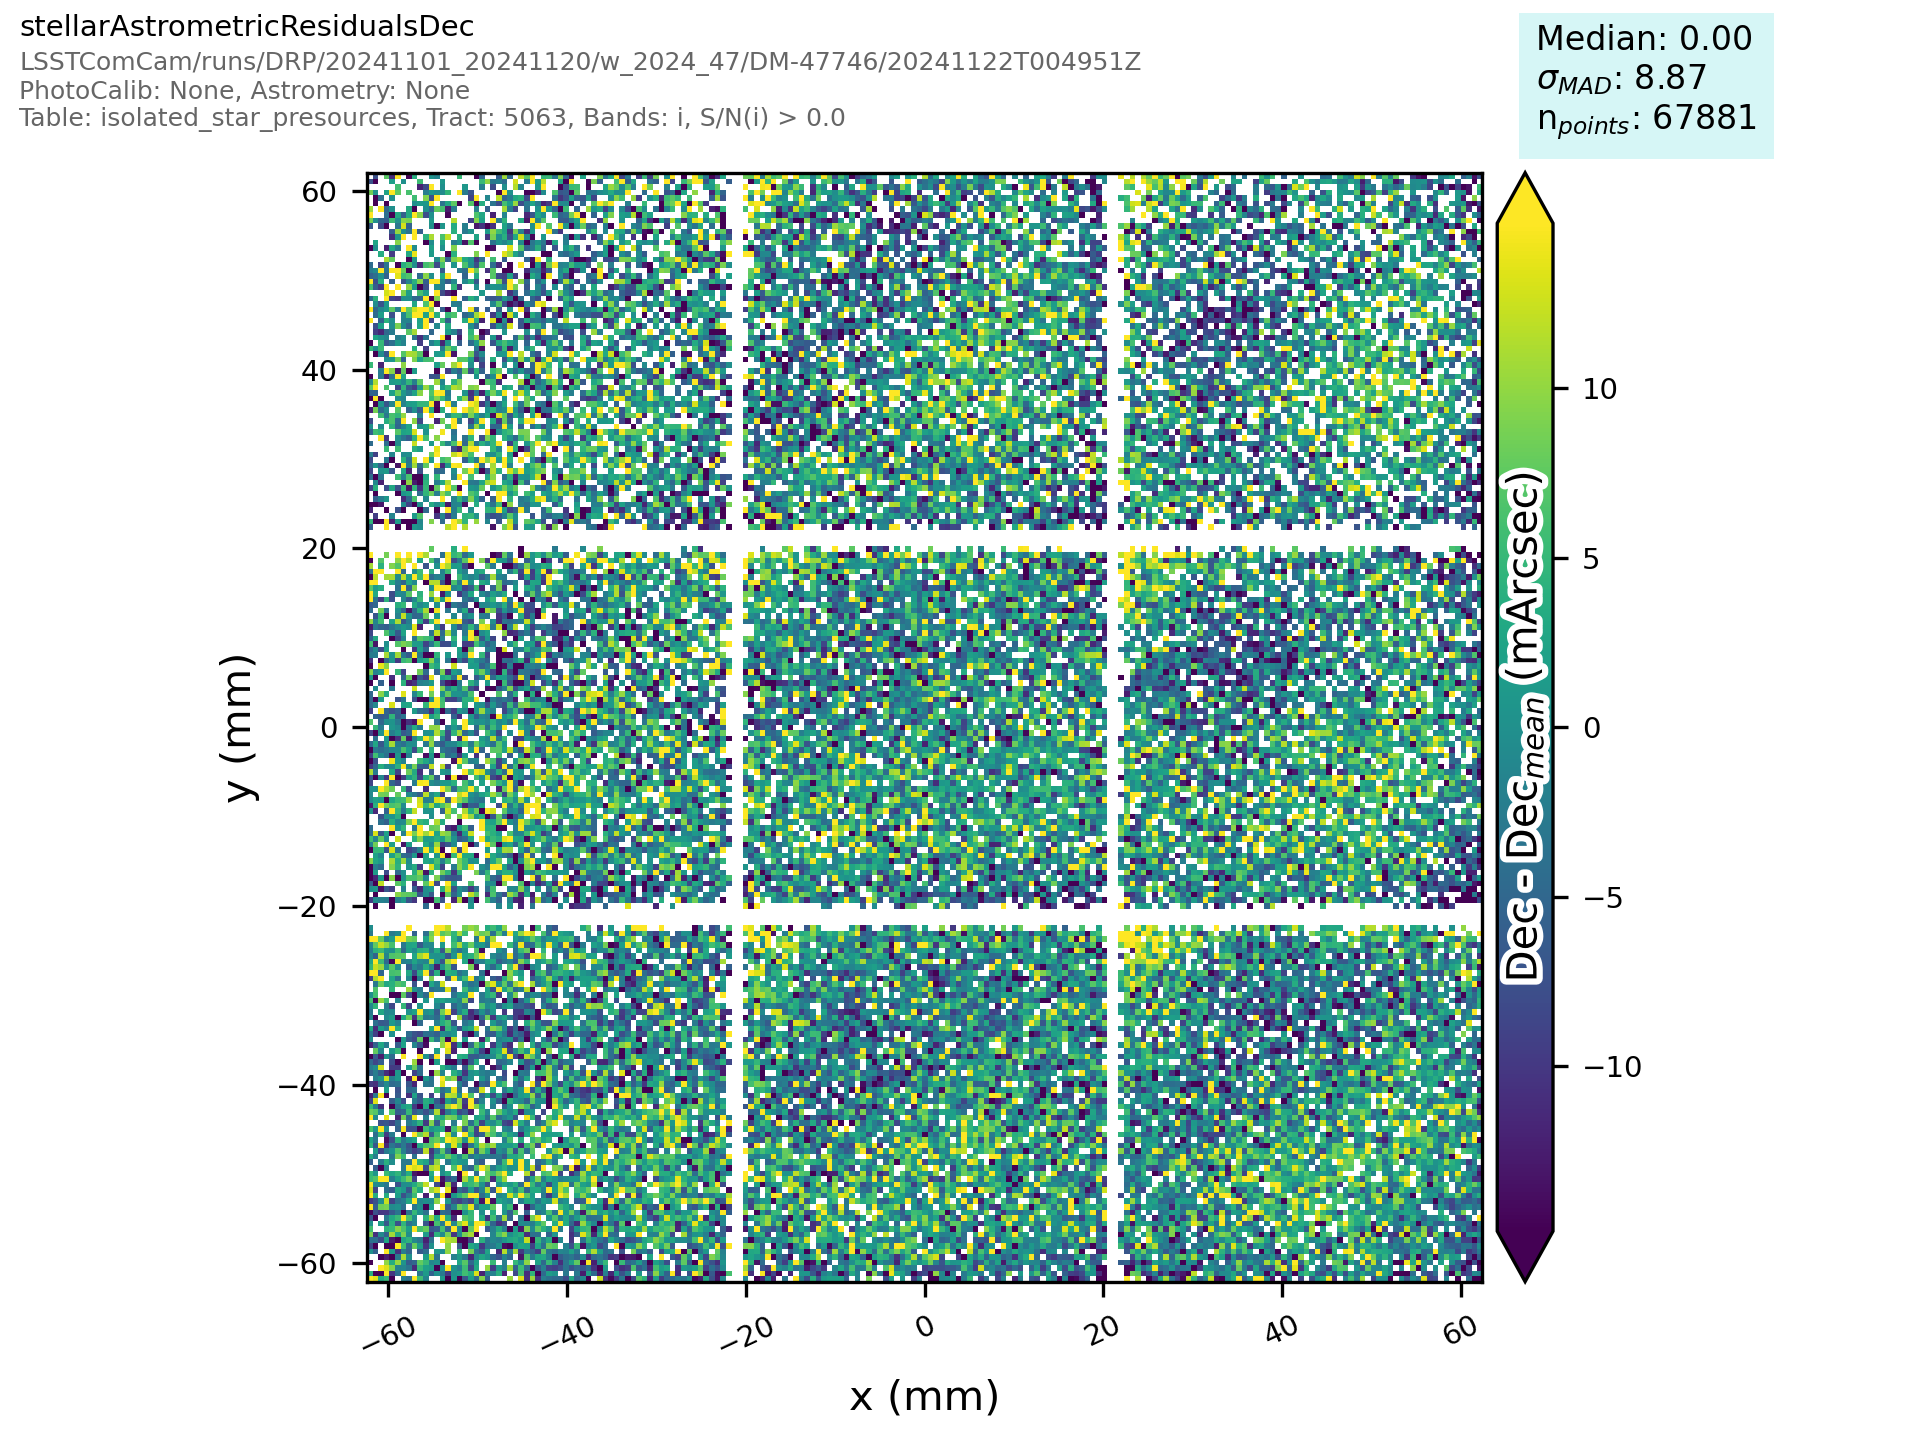
\includegraphics[scale=0.47]{figures/e3aea76f-3ed1-4686-9a24-00abf0ff9515}
        \caption{\small Declination residuals projected in Focal plane coordinate for a given tract. Some structure looks to be present in focal plane coordinates, which will be taken into account with GBDES. }
        \label{fov_astrometry_plot}
\end{figure*}


\subsection{Photometric Calibration}
\label{sec:photometric_calibration}

We have started commissioning the full photometric calibration pipeline for
Rubin Observatory, with great success so far. For testing photometric
calibration we have obtained over 150 dithered science observations in ugriz
over part of the Extended Chandra Deep Field-South (ECDFS) (one of the planned LSST
deep fields), and tens more in rizy over part of the Euclid Deep Field South
(EDFS). All of the science data has delivered seeing of $\sim0.8$ to $\sim1.5$
arcsecond seeing.  The
validation work in this document covers the ECDFS field with its more complete
filter coverage.

The precision photometric calibration software used for Rubin is the Forward
Global Calibration Method (Burke, Rykoff, \etal 2018) which was used
successfully to achieve better than 2 mmag uniformity for the Dark Energy
Survey. This software has been adapted for the LSST Science Pipelines and has
been used on Hyper Suprime Cam Special Survey Program (HSC SSP) for data
releases since DR2.
The performance on HSC data has not been as good as that on DES data due to a
number of reasons, yielding repeatability and uniformity closer to the 5 mmag
level for grizy data.

\iffalse                                % re HSC
First, we have had a lot of problems with HSC
backgrounds and amp-to-amp non-linearities.  Second, the HSC survey strategy
was not well suited to self calibration due to the slow slewing of the
telescope and the long time required to change a filter, leading to lots of
isolated single-band single-night surveys.  Third, we do not have detailed
throughput scans including detector-to-detector QE variations and in-situ scans
of the significant filter variations that are required for the full forward
modeling in FGCM.
\fi

Early calibration of the ComCam data is in many ways easier than that of HSC.
First of all, we have a smaller camera (9 detectors) and thus fewer variations
to have to cross-calibrate.  Second, the camera is situated in the center and
easiest to calibrate part of the focal plane.  Third, we only have one field to
calibrate across a few nights of data so far over a limited range of airmass.
Fourth, the survey strategy (multiple bands per night dithered and repeated
with overlapping filters from night to night) is well suited to
self-calibration.  On the other hand, we do not yet have
detailed filter or detector scans available for ComCam using the CBP (\secRef{cbp}), and are
therefore using the LSSTCam reference filter curves and average detector
throughput for the LSSTCam ITL detectors.  In addition, we do not have a flat
field screen so we have had to rely on twilight flat observations for flat fielding.

\subsubsection{Processing Overview}

We start with the standard ISR as documented in \secRef{isr}. While
there are a number of challenges that we have discovered with the ITL
detectors, these are mostly near the sky level, while the testing of
photometric calibration is focused on brighter stars that are less affected by
these issues. We then apply twilight flats, which we are investigating how to
make better. At the same time, we are going to have the flat field screen and
laser and projector installed prior to the commissioning of LSSTCam, so we do
not want to spend too much time worrying about specific challenges of twilight
flats which are only necessary for ComCam.

After flat fielding we find an initial point-spread function (PSF), do a star
selection based on source and psf moments that was developed for HSC
single-frame processing, and perform an initial astrometric solution and
photometric solution (with a single zero-point per detector).  The initial
astrometric solution is used to associate star observations together prior to
global photometric calibration with FGCM.  The initial photometric solution is
used for rapid analysis and prompt processing, but is not used at all for FGCM
which relies entirely on instrumental fluxes (in units of electrons) with a
minor constraint from the reference catalog.

\subsubsection{Global Photometric Calibration with FGCM}

All associated stars with observations with signal-to-noise greater than 10 are
input into the FGCM solution.  In addition, reference stars from The Monster
reference catalog are associated with the stars.  Only a small fraction of the
reference stars are used in the FGCM solution, sufficient to estimate an
``absolute'' calibration (trusting that The Monster is a good absolute
reference catalog).  There is additional ongoing work with absolute calibration
with respect to the CalSpec star C26202 which is not saturated in LSST images
and is fortunately contained in ECDFS that is described in \secRef{C26202}.

The FGCM model constrains the atmospheric parameters per night, as well as the
absolute throughput relative to the input scans.  The standard atmosphere is
given by MODTRAN, run at the elevation of Cerro Pachon at airmass 1.2 with an
Angstrom aerosol model.  The optics and filters are all taken from
\texttt{lsst/throughputs} version 1.9, and the detector throughput is taken from the
ITL average of the lab scans ingested into \texttt{obs\_lsst\_data}.  Note that the
detector QEs are normalized to 1.0 at 800 nm, which is certainly
greater than the true QE at this wavelength.

\subsubsection{FGCM Results on the ECDFS Field}

The FGCM results presented here are based on the
\texttt{LSSTComCam/runs/DRP/20241101\_20241113/w\_2024\_46/DM-47566} DRP processing
run, specifically the 157 visits overlapping tracts
4847, 4848, 4849, 5062, 5063, 5064 which are in the ECDFS field. Specifically there
are 28, 18, 38, 45, 28 visits in ugriz respectively. All QA plots are available
in \href{https://usdf-rsp.slac.stanford.edu/plot-navigator}{the plot navigator at USDF} in
the collection \texttt{u/erykoff/LSSTComCam/DM-47303/test2/build2/run9}.  In this
section we focus on some of the highlights.

Note that FGCM defines a ``photometric'' observation as one that is consistent
with the forward model, including normal variations in the atmosphere, airmass,
known detector throughputs, filter curves, and additional accomodation for
aperture corrections (discussed in Burke, Rykoff \etal).  With this definition
fully 92\% of the observations were deemed to be photometric by the code.

\subsubsubsection{Illumination Corrections}

Part of the FGCM solution is generating illumination correction maps (\figRef{illumination_correction})
with a second-order 2D Chebyshev polynomial over each detector.  Prior to LSSTCam
commissioning this will be turned into a separate calibration product generated
from dense dithered star field observations (Y1).
We have not yet done dithered observations with ComCam over a dense
field, only high latitude, which limits the precision.  Nevertheless we are
able to constrain reasonable illumination corrections.  The offsets from
detector to detector in the illumination correction are due to unexpected
offsets in the twilight flats that we are investigating.

\begin{figure}
  \begin{center}
    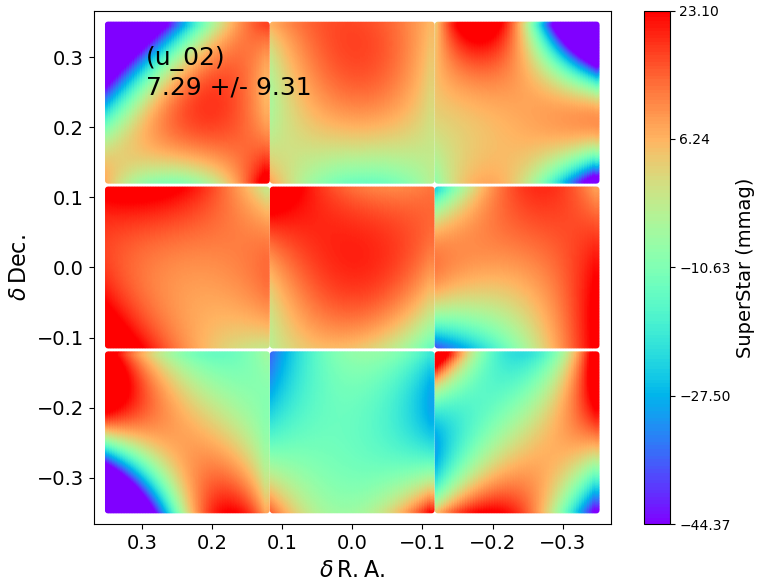
\includegraphics[width=0.3\textwidth]{photometric_calibration_figures/illumcorr_u.png}
    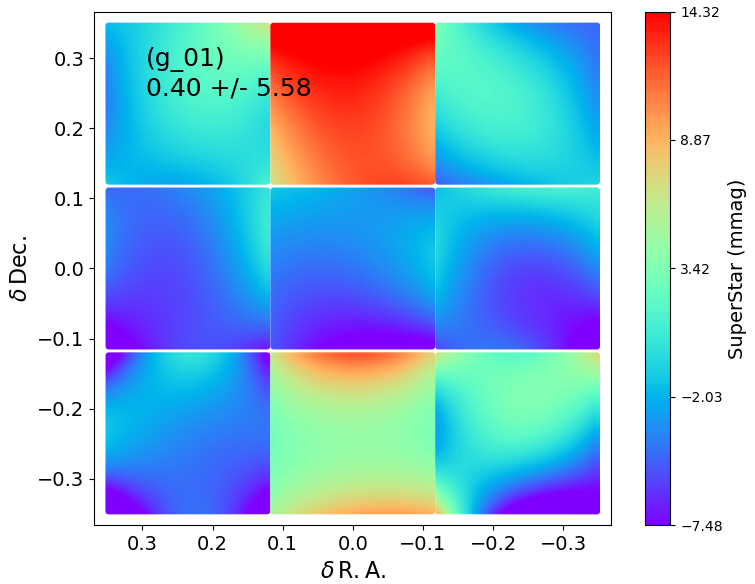
\includegraphics[width=0.3\textwidth]{photometric_calibration_figures/illumcorr_g.png}
    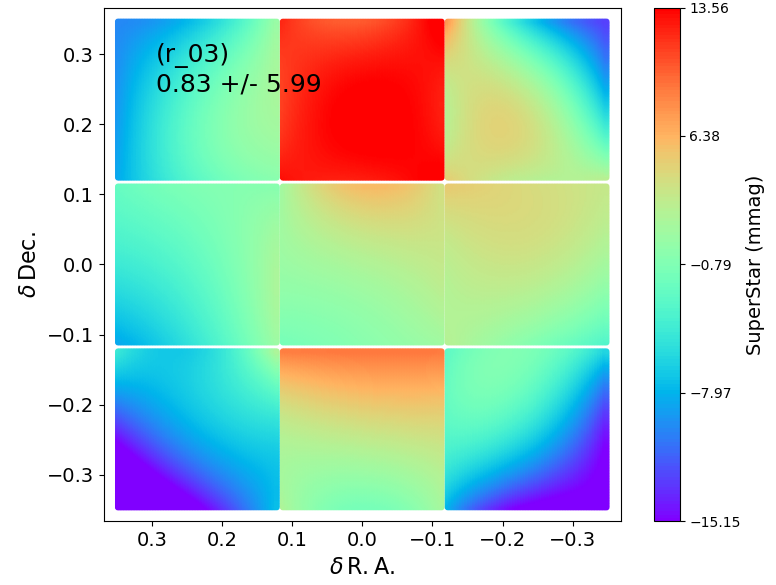
\includegraphics[width=0.3\textwidth]{photometric_calibration_figures/illumcorr_r.png}
    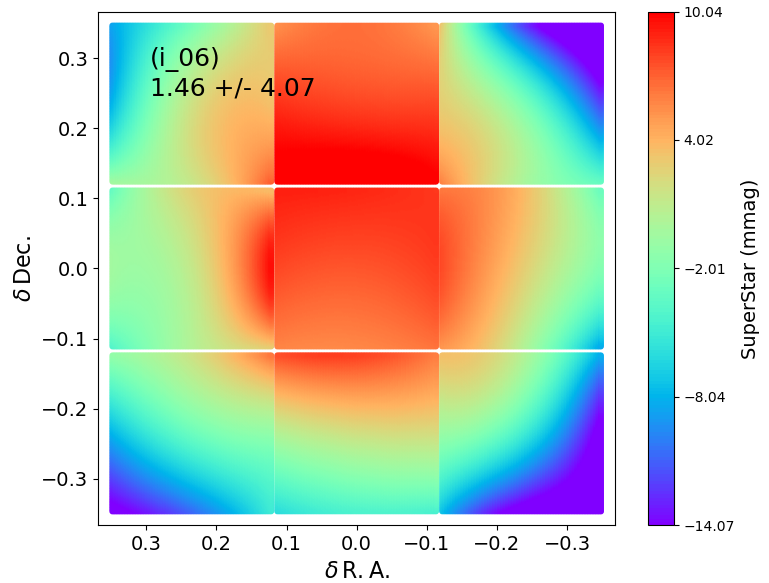
\includegraphics[width=0.3\textwidth]{photometric_calibration_figures/illumcorr_i.png}
    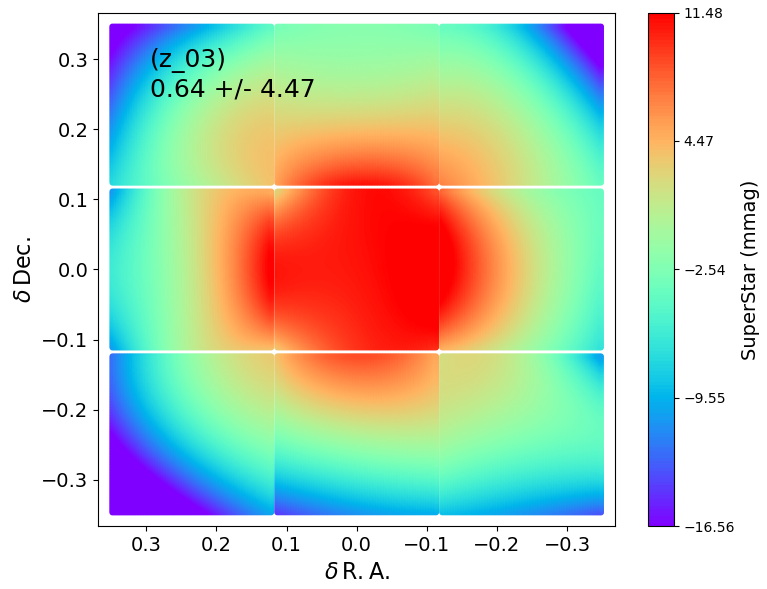
\includegraphics[width=0.3\textwidth]{photometric_calibration_figures/illumcorr_z.png}
  \end{center}
  \caption{Illumination corrections derived from FGCM for the ugriz bands.}
  \label{fig:illumination_correction}
\end{figure}

\subsubsubsection{Photometric Repeatability}

The photometric repeatability after the FGCM fits was excellent. We show here
the repeatability histograms, after all chromatic corrections, for the stars
used in the fit (``all stars'').  Although 10\% of the stars are reserved,
the histograms do not yet have good statistics.  These plots are all made with
signal-to-noise greater than 100 stars (with better than 1\% photometric
errors).  Therefore the scatter is often dominated by photometric error.  The
label ``sigma\_fgcm`` is meant as an estimate of the intrinsic scatter after
subtracting off the photometric error in quadrature. The plots are split into
four panels, showing all stars, the 25\% bluest (from $g-i$ color), the 50\%
middle color, and the 25\% reddest stars. Note that the reddest stars tend to
be fainter and thus have larger photometric error. Furthermore, there are no
red stars observed in the u-band. In all cases except the u-band the intrinsic
repeatability is $1\,\mathrm{mmag}$ or better, and for the u-band it is better
than $5\,\mathrm{mmag}$, comfortably exceeding our requirements in all measured bands.

\begin{figure}
  \begin{center}
    \includegraphics[width=0.3\textwidth]{photometric_calibration_figures/repeatability_u.png}
    \includegraphics[width=0.3\textwidth]{photometric_calibration_figures/repeatability_g.png}
    \includegraphics[width=0.3\textwidth]{photometric_calibration_figures/repeatability_r.png}
    \includegraphics[width=0.3\textwidth]{photometric_calibration_figures/repeatability_i.png}
    \includegraphics[width=0.3\textwidth]{photometric_calibration_figures/repeatability_z.png}
  \end{center}
  \caption{Photometric repeatability for stars in the ugriz bands.}
\end{figure}

\subsubsubsection{Detector Chromaticity Fits}

In the absence of full in-situ throughput scans, we additionally constrain the
``chromaticity'' of the detectors, which is a first-order adjustment to the
slope of the peak of the throughput curve per-detector.  By doing this
adjustment in throughput space rather than color space we can preserve the
forward model approach, and additionally apply these corrections to any
SED. Note that this operation assumes that the filters are perfectly known, and
it is only the detector throughput that is varying.  This is, in general, a
valid assumption in the g band where the AR coating varies from detector to
detector causing chromatic differences in this band.

\begin{figure}
  \begin{center}
    \includegraphics[width=0.6\textwidth]{photometric_calibration_figures/detector_chromaticity_g.png}
  \end{center}
  \caption{Variation in throughput in the g band for the 9 ComCam detectors as
    derived from star colors. These are all constrained relative to the average
    ITL throughput. The CBP will be used for making this measurement
    ``correctly'', but this serves as a prediction of what variations the CBP
    scans should observe when we have it running on ComCam.}
\end{figure}

\subsubsubsection{Absolute Throughputs}

The FGCM fit performs a ``dead reckoning'' of the expected absolute throughput
given the telescope aperture, the effective gain, the standard atmosphere, and
the various throughputs input.  See above for the throughputs assumed.  If we
trust The Monster reference catalog for absolute calibration,
\figRef{absthroughputs} shows the comparison of the delivered
throughput to the predicted throughput.  In griz bands it is very close, given
that (a) we know that the peak detector QE is not 100\%; and (b) the ComCam
front lens did not have an AR coat applied, thus reducing its throughput
relative to nominal LSSTCam lenses.  In u band we are getting more throughput
than predicted.  This may be an issue with the reference catalog, or our ComCam
u-band QE is 20-30\% larger than the baseline expectation.  Given how fast the
detector QE falls off in the u-band, it would not take much to increase the
throughput by this factor.

\begin{figure}
  \begin{center}
    \includegraphics[width=0.6\textwidth]{photometric_calibration_figures/abs_throughput.png}
  \end{center}
  \caption{Absolute throughput derived per band, relative to naive expectations.}
  \label{fig:absthroughputs}
\end{figure}

We have additional ongoing studies of absolute throughputs using the CalSpec
standard C26202 directly.

\subsubsubsection{Comparison to The Monster}

Given our calibrated stars from the FGCM fit we can compare the magnitudes as a
function of color against The Monster reference catalog.  The ``lsst'' fluxes
in The Monster were derived by using stellar spectra to convert from The
Monster native DES system to the standard throughputs in lsst/throughputs
v1.9. These do not match ComCam, in particular it used a strange hybrid of
ITL/E2V for the detector throughput, which is not correct for
ComCam. Therefore, we do expect residual color terms.  Studies are ongoing on
whether these color terms are expected given the differences between the ComCam
throughput and the predicted LSST throughput.  Further validation will be
possible if we get CBP scans prior to the removal of ComCam.

\begin{figure}
  \begin{center}
    \includegraphics[width=0.3\textwidth]{photometric_calibration_figures/reference_residuals_u.png}
    \includegraphics[width=0.3\textwidth]{photometric_calibration_figures/reference_residuals_g.png}
    \includegraphics[width=0.3\textwidth]{photometric_calibration_figures/reference_residuals_r.png}
    \includegraphics[width=0.3\textwidth]{photometric_calibration_figures/reference_residuals_i.png}
    \includegraphics[width=0.3\textwidth]{photometric_calibration_figures/reference_residuals_z.png}
  \end{center}
  \caption{Residuals between FGCM standardized magnitudes and The Monster
    predicted LSST magnitudes for the ugriz bands as a function of $g-i$, assuming
    The Monster has the correct absolute throughput.}
\end{figure}

\subsubsubsection{Background Oversubtraction}

As a side-effect in the calibration, FGCM tests local background
oversubtraction by looking at the statistical difference between two large
aperture magnitudes.  If the background were perfectly measured then the
difference in magnitude will just be a measure of the wings of the PSF (a local
portion of the growth curve) which should be self-similar for all star fluxes.
Instead, we generally see a downturn consistent with a constant background
offset.  This background oversubtraction has been seen in DES, HSC, and
ComCamSim data at similar levels with different photometric pipelines.  It is
worse in the redder bands.  It seems to be caused by the far wings of stars (in
DES all stars and galaxies brighter than 17th magnitude in i contribute), as
well as possibly due to faint undetected sources.  This same background
oversubtraction effect is seen in the ComCam images.  Further investigations
are being done by the low-surface-brightness science unit.

\begin{figure}
  \begin{center}
    \includegraphics[width=0.3\textwidth]{photometric_calibration_figures/background_oversubtraction_u.png}
    \includegraphics[width=0.3\textwidth]{photometric_calibration_figures/background_oversubtraction_g.png}
    \includegraphics[width=0.3\textwidth]{photometric_calibration_figures/background_oversubtraction_r.png}
    \includegraphics[width=0.3\textwidth]{photometric_calibration_figures/background_oversubtraction_i.png}
    \includegraphics[width=0.3\textwidth]{photometric_calibration_figures/background_oversubtraction_z.png}
  \end{center}
  \caption{Estimate of the background oversubtraction using delta magnitudes
    from large apertures in the ugriz bands.  The amount of curvature is a measure
    of the oversubtraction; this should be flat as a function of star magnitude
    if the background were measured correctly on average.}
\end{figure}

\begin{figure}
  \begin{center}
    \includegraphics[width=0.9\textwidth]{photometric_calibration_figures/background_oversubtraction_g.png}
  \end{center}
  \caption{Estimate of the background oversubtraction using delta magnitudes
    from large apertures in the g band.  The amount of curvature is a measure
    of the oversubtraction; this should be flat as a function of star magnitude
    if the background were measured correctly on average.}
\end{figure}

\begin{figure}
  \begin{center}
    \includegraphics[width=0.9\textwidth]{photometric_calibration_figures/background_oversubtraction_r.png}
  \end{center}
  \caption{Estimate of the background oversubtraction using delta magnitudes
    from large apertures in the r band.  The amount of curvature is a measure
    of the oversubtraction; this should be flat as a function of star magnitude
    if the background were measured correctly on average.}
\end{figure}

\begin{figure}
  \begin{center}
    \includegraphics[width=0.9\textwidth]{photometric_calibration_figures/background_oversubtraction_i.png}
  \end{center}
  \caption{Estimate of the background oversubtraction using delta magnitudes
    from large apertures in the i band.  The amount of curvature is a measure
    of the oversubtraction; this should be flat as a function of star magnitude
    if the background were measured correctly on average.}
\end{figure}

\begin{figure}
  \begin{center}
    \includegraphics[width=0.9\textwidth]{photometric_calibration_figures/background_oversubtraction_z.png}
  \end{center}
  \caption{Estimate of the background oversubtraction using delta magnitudes
    from large apertures in the z band.  The amount of curvature is a measure
    of the oversubtraction; this should be flat as a function of star magnitude
    if the background were measured correctly on average.}
\end{figure}

\subsubsection{Next Steps}

The following additional data will need be taken to advance from our current
knowledge:

\begin{enumerate}
  \item{g band observations in the EDFS field, when the g filter is put back
    into ComCam for the upcoming dark time.}
  \item{Dithered observations in as many bands as possible over a field with
    much larger stellar density for better illumination corrections.}
  \item{More contiguous dithered survey data in (at least) gri.}
\end{enumerate}

The particular emphasis on g band in these requests is that by default FGCM
will use the $g-i$ color for internal QA, which is a very useful color to split
on.  There are no facilities in the code for doing quality calibrations on
multiple disconnected fields with different band coverage, as this is not the
normal case for survey observations.  We could run different fields separately
with different configs, but this is not preferred.  Thus, gri coverage over the
fields of interest for DRP processing is the ``easiest'' path that will yield
the best results and be most consistent with the LSST survey.


\subsection{A Comparison with the HST CalSpec Standard C26202}
\label{sec:C26202}

The CDFS field observed by ComCam during commissioning contains an HST
CalSpec standard that is faint enough not to saturate the ComCam
science images.  This HST CalSpec
standard\footnote{\url{https://www.stsci.edu/hst/instrumentation/reference-data-for-calibration-and-tools/astronomical-catalogs/calspec}},
C26202, had previously been used to perform the absolute AB
calibration of the Dark Energy Survey (DES) Data Release 2 (DR2)
\citep{2021ApJS..255...20A}.

For the ComCam data, two separate (but related) analyses were
performed using the ComCam observations of C26202: (1) a measurement
of the absolute system throughput of the ComCam $ugrizy$ bandpasses,
and (2) a measurement of how far off the initial absolute photometric
calibrations were from the AB magnitude system (``AB offsets'') for
these same bandpasses.

These two analyses are discussed below.

\subsubsection{Absolute System Throughput Measurements}

For the absolute system throughput analysis, the expected total counts
(in electrons) for C26202 were calculated for each of the ComCam
bandpasses for a 30-second exposure, assuming the engineering system
throughputs for an average ITL CCD found in the {\tt
  syseng\_throughputs repository} (see
\url{https://github.com/lsst-pst/syseng\_throughputs}). Expected
counts in each filter passband were calculated for a range of
airmasses ($1.0 \leq X \leq 2.5$) in steps of 0.1 airmass to cover the
full range of possible airmasses of the observed ComCam data.
Throughout, the HST CalSpec spectral energy distribution (SED), {\tt
  c26202\_stiswfcnic\_007.fits}, was used as the C26202
spectrophotometric reference spectrum.

Next, the post-ISR instrumental counts (in electrons) for C26202 were
retrieved from the {\tt icSrc} tables from the ComCam observations in
the Butler at the USDF.  The {\tt base\_PsfFlux\_instFlux} was used,
and an aperture correction from PSF to total flux was applied making
use of the {\tt base\_CircularApertureFlux\_70} as a proxy for total
instrumental flux.

Finally, for each of the $ugrizy$ filter passbands, the ratio of the
observed total flux to the expected (synthetic) total flux was
calculated and plotted.  The results can be found in
Figure~\ref{fig:c26202_throughputs}.  Note that the measured and
predicted counts from per-visit synthetic photometry is consistent for
all bands at the $\sim$5\% level.

\begin{figure}
  \begin{center}
    \includegraphics[width=0.7\textwidth]{photometric_calibration_figures/LSSTComCam_Absolute_Throughputs_20241210.png}
  \end{center}
  \caption{\label{fig:c26202_throughputs}The histogram of the ratio of
    the observed counts to the expected counts for HST CalSpec
    spectrophotometric standard star C26202 from ComCam observations
    in {\tt
      LSSTComCam/runs/DRP/20241101\_20241204/w\_2024\_49/DM-47988}.
    Median values of the ratio for each passband are: 1.053 ($u$),
    0.939 ($g$), 1.068 ($r$), 1.037 ($i$), 1.037 ($z$), and 0.967
    ($y$).}
\end{figure}


\subsubsection{AB Offsets}

The C26202 AB magnitude offsets are the difference between the
calibrated observed ComCam AB magnitudes and the {\tt
  rubin\_sim.PhotUtils}-determined synthetic AB magnitudes for the
ComCam $ugrizy$ filter passbands.

The calibrated ComCam AB magnitudes in each of the passbands are
obtained by converting the {\tt calibFlux} values in the USDF butler
{\tt sourceTable} from nano-Janskys to AB magnitudes via the equation
$mag_{\rm ab} = -2.5 \times log_{10}(calibFlux)$.

As with the absolute system throughput measurements for the expected
counts of C26202, the engineering system throughputs for an average
ITL CCD found in the {\tt syseng\_throughputs repository} were used
for calculating the expected AB magnitudes with the {\tt rubin\_sim
  PhotUtils} module for each filter bandpass.  Also, as with the
absolute system throughput measurements, the HST CalSpec spectral
energy distribution (SED), {\tt c26202\_stiswfcnic\_007.fits}, was
used as the C26202 spectrophotometric reference spectrum.

The results are shown in Figure~\ref{fig:c26202_ab_offsets}.

These results are not unexpected, as performing absolute calibrations
on reference catalog data is extremely difficult before real observed
data are obtained in a new filter bandpass system.  Updates are now
being applied by the Rubin Calibration Scientist to address these
offsets.


\begin{table*}
\centering
\begin{tabular}{@{}lcccc@{}}
  Band & No. of \ComCam observations & median \ComCam mag. & CalSpec synthetic mag. & offset \\
  \hline
u             & 28  & 17.869 & 17.573 &  $\phantom{-}0.296$ \\
g             & 77  & 16.684 & 16.692 &  $          -0.008$ \\
r             & 121 & 16.269 & 16.362 &  $          -0.093$ \\
i             & 99  & 16.197 & 16.260 &  $          -0.063$ \\
z             & 42  & 16.589 & 16.244 &  $\phantom{-}0.346$ \\
y             & 24  & 16.269 & 16.239 &  $\phantom{-}0.031$ \\
\end{tabular}
\caption{Comparison of \ComCam observed magnitudes with synthetic magnitudes calculated from
  C26202\_stiswfcnic\_007 using \ComCam passbands.
}
\label{tab:C26202}
\end{table*}

%HST CalSpec Standard observed in ECDFS field

%DRP Cumulative collection \texttt{LSSTComCam/runs/DRP/20241101_20241204/w_2024_49/DM-47988}
%ComCam observed mags are from the calibFlux values from the sourceTable

%ComCam ugrizy synthetic mags generated using rubin_sim.PhotUtils and syseng_throughput
%ComCam ITL responses used.

%There are 2 related-but-separate analyses going on:  the AB offset analysis here, and 
%the throughput analysis.
%The AB offset analysis is just concerned about the difference in the calibrated observed 
%ConCam AB magnitudes and the synthetic AB magnitudes.  We get the calibrated ConCom AB 
%magnitudes from the calibFlux column of the sourceTable and converting the calibFlux 
%(in nano-Janskys) to AB magnitudess via mag_ab = -2.5*log10(calibFlux).   I believe — 
% but am not 100% certain — that the calibFlux values in the sourceTable have been 
%photometrically calibrated against the Monster RefCat, probably via calculating a local 
%photometric zeropoint from the Monster stars observed by ConCam in that visit+detector.  
%If this is the procedure for the photometric calibration of the calibFlux column of the 
%sourceTable, the first-order airmass correction (the k*X term in SDSS parlance) is taken 
%care of automatically, since the Monster RefCat stars are observed through the same airmass 
%for that  visit+detector.  For the synthetic AB magnitudes, essentially Equation 7 of 
%Fukugita \etal (1996) is used.  The shape of the passbands is important, but the total 
%throughput cancels out.  For the ConCam-based synthetic magnitudes, I used the rubin_sim 
%PhotUtils module and the syseng_throughput package (in order to make use of the ConCam 
%ITL responses), following code that Lynne Jones pointed me to.  (I think the default 
%airmass is X=1.2 or X=1.3; I am not sure, but it shouldn’t make a bit difference in the 
%overall shape of the passbands.) So, if the passband shapes (including atmosphere, etc.) 
%are generally well known and if the calibFlux is indeed calibrated against the Monster 
%RefCat,  but there is an overall AB magnitude offset, I think this would imply a possible 
%AB calibration error in the Monster RefCat.

%The total throughput analysis ignores the Monster entirely.  It takes the ISR-corrected 
%(but not photometrically zeropointed) psf instFlux counts for C26202 from the icSrc 
%table and compares them against the expected counts for a single 30-second exposure 
%calculated via rubin_sim PhotUtils module and the syseng_throughput package, again 
%making use of code that Lynne provided.  In this case, estimaging total throughput 
%is critical to the analysis — in fact, it is the purpose of the analysis.   Here, 
%the expected counts are corrected to the airmass of the visit, and not just to a 
%typical/official airmass like in the AB offset analysis above.


\section{Survey Performance}
\label{sec:survey_performance}

Understanding and predicting survey performance includes modeling the likely input telemetry, the expected performance of the telescope and observatory, as well as understanding the survey strategy and its interaction with science outcomes. 

At this point in commissioning, the operations of the observatory are focused on obtaining specific observations, with very different strategies than will be employed during operations. This includes very different configurations of the Feature Based Scheduler. Thus, we are not testing the Feature Based Scheduler as it would be used in operations yet, and have no comment about issues that may be related specifically to survey strategy implementation. 

We can however begin to evaluate how our models may be validated or not by the currently acquired observations. We focus on the observations acquired for the science program, BLOCK-320.

First, clearly bad visits (where stars were clearly trailed in the images, as visible in rubintv) were removed from the set of science visits. 

The throughput curves available in `syseng_throughputs`, the repository that tracks current system engineering summaries of full-focal-plane throughputs, can be used to predict zeropoints for average ITL CCDs. See \url{https://github.com/lsst-pst/syseng_throughputs/blob/main/notebooks/InterpolateZeropoint.ipynb}, where a simple interpolation function for filter and airmass is defined for the current throughputs (v1.9). The returned zeropoint includes the exposure time, as zeropoints in DM pipelines outputs are for a given exposure with the given exposure time (they are not 1-second zeropoints). A comparison of these predicted zeropoints to the reported median visit zeropoints in the ConsDB (the column `cdb_lsstcomcam.visit1_quicklook.zero_point_median`) is shown in Figure~\ref{fig:zeropoints). The mean of these zeropoint variations averages 0.13 magnitudes across all bands, being slightly smaller in r (0.09 mag) and slightly larger in y band (0.18); the RMS scatter in these measurements is < 0.02 magnitudes. 

\begin{figure}
    \centering
    \includegraphics[width=0.8\textwidth]{sp/zeropoints.png}
    \caption{Predicted zeropoints from syseng_throughputs (accounting for airmass) compared to measured zeropoints from `cdb_lsst.comcam.visits1_quicklook`.}
    \label{fig:zeropoints}
    \end{figure}

\section{Sample Production}
\label{sec:sample_production}

\section{Difference Image Analysis: Transience and Variable Objects}
\label{sec:dia_transient_variable}


\subsection{DIA Status}

As we have started to obtain repeated science-quality images of some fields, we have begun to build coadded templates as part of the regular weekly cumulative Data Release Processings. 
These mini-DRPs also include difference image analysis (DIA) of their constituent exposures.
Using the DRP-produced templates, we have also obtained near-real-time difference images in Prompt Processing for a few exposures. 
We have not yet had the opportunity to begin tuning template generation, difference imaging, or Real/Bogus characterization of these data, so the report below provides an initial rough characterization of DIA performance. 

\subsection{ML Reliability and Artifact Rates}

We ran a convolutional neural network on 51$\times$51 difference, science, and template cutouts for 912k DIASources identified in the \texttt{w\_2024\_47} data release processing.  
This processing primarily includes data from extragalactic deep fields.
These DiaSources were obtained from 4252 detector-visit images, implying an average of 21 DIASources per detector or about four thousand per equivalent full LSST focal plane.
This is somewhat less than the ten thousand DIASources expected per visit and may reflect lower sensitivity due to ongoing image quality refinement and early templates.

The CNN was trained on simulated DC2 images with additional point source injection, so caution is needed when interpreting the values returned by this classifier on ComCam data.
Nevertheless,  Figure \ref{fig:reliability_hist} shows a clear separation in reliability scores and would imply roughly a 3:1 bogus:real ratio if taken at face value.
These values will be confirmed with manual inspection.
We plan to train a purpose-built classifier on larger samples of labeled ComCam data.

\begin{figure}
\includegraphics[width=\textwidth]{dia/figures/reliability_histogram.png}
\caption{Histogram of machine-learned reliability scores computed on ComCam difference images. \label{fig:reliability_hist}}
\end{figure}

\section{Difference imaging QA}

\begin{figure}
\includegraphics[width=\textwidth]{Diffim kernel quiver plot.png}
\caption{Quiver plot of the implied offset between the science and template images, calculated from the centroid of the PSF matching kernel. \label{fig:diffim-quiver}}
\end{figure}

A difference imaging afterburner is run manually on Prompt Processing output to generate diagnostic plots, such as \ref{fig:diffim-quiver}.
From \ref{fig:diffim-quiver} we see the centroid of the PSF matching kernel sampled across one detector, which reveals a systematic offset between the science and template images.
A similar offset is seen across the rest of the detectors for this visit, and in other visits.
The images comprising the template used the same astrometric reference catalog as the science image in this case, but the template was constructed with the calibrate+characterizeImage pipeline while the science image was processed with calibrateImage.
These are not included in the Prompt Processing payload to save critical time during observing.

The distribution of sources detected on the difference image reveals some detector-level effects that are not fully accounted for.
Binning the locations of the diaSources in 1-D in \ref{fig:diaSource-distribution} by their x- and y-values reveals systematic overdensities of detections at the amplifier boundaries in x (but not in y).
Additional overdensities seen in y-band may be from the residual phosphorescent wax reported to be left on some chips beneath the AR coating.

\begin{figure}
\includegraphics[width=\textwidth]{diaSource_distribution.png}
\caption{Binning the locations of the diaSources in 1-D by their x- and y-values reveals systematic overdensities of detections at the amplifier boundaries in x (but not in y). \label{fig:diaSource-distribution}}
\end{figure}

\subsection{Cosmic Ray Detection Performance}

In this analysis, we evaluate the performance of the cosmic ray detection algorithm by integrating real cosmic ray events into simulated observational data and applying standard detection pipelines to assess their performance. The primary objective is to assess the algorithm's ability to accurately identify cosmic rays, thereby ensuring data purity for subsequent scientific analyses.

\subsubsection{Methodology}

We used 67 visits (603 detectors), where the dark frames were taken from 2024-10-27 to 2024-11-01, and the simulated exposures are from $day\_obs=20240626$.

We processed a set of simulated on-sky images from the ComCamSim OR4 repository and added real ComCam dark frames containing only cosmic rays. First, we performed Instrument Signature Removal (ISR) on ComCam darks as well as ComCamSim separately. After that, we combined the two images and performed image characterization and calibration.

To establish ground truth, we used the ComCam dark frames and identified pixels that were brighter than 5 times the standard deviation above the mean background level. This threshold allowed us to create a ground truth mask representing cosmic rays. At the end of the process, we compared this ground truth mask with the cosmic ray (CR) mask obtained after the characterization step to evaluate the algorithm's performance.

\subsubsection{Results}

The detection outcomes were categorized into four classes: True Positives (TP), False Positives (FP), True Negatives (TN), and False Negatives (FN). The counts for each category are presented in Table~\ref{tab:confusion_matrix}. The True Positives, False Positives, True Negatives, and False Negatives represent the comparison between the CR mask and the ground truth mask. Critical False Negatives (CFN), on the other hand, are the pixels that are considered detections (from the DETECTED mask) but are, in fact, cosmic rays.

\begin{table}[H]
    \centering
    \caption{Confusion Matrix for Cosmic Ray Detection (Pixel counts)}
    \label{tab:confusion_matrix}
    \begin{tabular}{*3c}
        \hline
        & \textbf{Positive (Detected)} & \textbf{Negative (Not Detected)} \\
        \hline
        \textbf{True (Cosmic Ray)}  & 223,982 & 92,366 \\
        \textbf{False (Non-Cosmic Ray)} & 86,094  & 9,821,261,558 \\
        \hline
         \multicolumn{2}{c}{\textbf{CFN (Cosmic Ray detected as Source)}} & 27954 \\
    \end{tabular}
\end{table}

From these results, we calculated the following performance metrics:

\begin{itemize}
    \item \textbf{Purity (Precision):} 
    \begin{equation*}
        \text{Purity} = \frac{TP}{TP + FP} = \frac{223,982}{223,982 + 86,094} \approx 0.722
    \end{equation*}
    \item \textbf{Completeness (Recall):} 
    \begin{equation*}
        \text{Completeness} = \frac{TP}{TP + FN} = \frac{223,982}{223,982 + 92,366} \approx 0.708
    \end{equation*}
    \item \textbf{Adjusted Completeness:} Considering critical false negatives (CFN), where cosmic rays were detected as sources, the adjusted completeness is 
    \begin{equation*}
        \text{Adjusted Completeness} = \frac{TP}{TP + CFN} = \frac{223,982}{223,982 + 27,954} \approx 0.889
    \end{equation*}
\end{itemize}

\subsubsection{Discussion}

The results indicate that the current cosmic ray detection algorithm demonstrates moderate success in identifying cosmic rays, as evidenced by a purity of approximately 72.2\%. This suggests that most of the detections are indeed true cosmic rays, though a significant portion, about 27.8\%, are false positives.

The completeness, at around 70.8\%, reveals that while the algorithm is capable of detecting a majority of cosmic rays, it still misses a substantial number of events. However, the adjusted completeness of 88.9\% highlights the algorithm's improved performance when considering critical false negatives—those cosmic rays that were detected but mistakenly classified as sources rather than cosmic rays. 



\subsection{Satellite Streaks}

As orbital space becomes increasingly crowded, we expect to see many bright streaks, flares, and glints due to satellites and other reflective human-made objects orbiting the Earth. The majority of the population is in low-Earth orbit (LEO). For a review of the current status and likely impacts to LSST, please see \url{ls.st/satcon}.

As expected, many ComCam detector-visit images clearly show streaks. Visual inspection of nearly all ComCam images to date are being recorded on a best-effort basis in a Confluence Database dubbed ``ComCam Satellite Spotter,'' and as of 2024 Nov 25 there are over 500 rows. The simple schema has one row per visit (if a streak crosses multiple detectors --- which it often does --- this is indicated in the ``detector'' column). In general, the morphology of streaks falls into one of these categories:
\begin{itemize}
\item Straight bright linear feature, typically at least 20 pixels wide, that crosses one or more detectors and goes off the edge (typical of most LEO satellites, such as Starlink)
\item Shorter version of the above, with clear start and/or endpoints, which usually indicates the object imaged is located at a higher-than-LEO orbital altitude (and/or the exposure integration time was unusually short)
\item Intermittent linear feature, i.e., a dashed line, due to different parts of the satellite having different reflective properties
\item A flare or glint brightening event that fades in and out along a linear trajectory, either isolated or as part of a longer streak
\item Actually a bright star diffraction spike
\item Actually a cosmic ray that was not repaired
\item Variation of any of the above but in out-of-focus donut form (interestingly, depending on altitude, certain streaks may appear either in- or out-of-focus when stars appear as donuts)
\end{itemize}

Thanks to ComCam's relatively small field of view and the satellite population being as small as it ever will be during Rubin Commissioning and Operations, we have not yet seen an overwhelmingly bright satellite (e.g., BlueWalker 3 or one of the BlueBirds, all operated by AST SpaceMobile). Only a couple instances have streaks bright enough to induce visually-obvious crosstalk ``secondary streaks;'' the majority of streaks are relatively faint and the only portion of the image impacted are regions overlapping with the streak itself on the sky. Reliably determining streak width is an ongoing challenge, as it is not a delta function, and some of the brighter streaks do have notably extended stray light profile wings.

We note the Science Pipelines' algorithmic approach to identifying linear streak features  (see \url{https://dmtn-197.lsst.io}) uses the detected mask plane and not the image array (pixel values) for efficiency. To more effectively detect faint streaks in difference images, as in the DECam example shown in Figure \ref{fig:decam-streak}, we have recently implemented a binning scheme designed to be sensitive to linear features that fall below the detection threshold.

\begin{figure}[ht!]
    \centering
    \includegraphics[width=0.5\linewidth]{figures/decam-streak.png}
    \caption{THIS IS DECAM, NOT COMCAM. A typical faint satellite streak in a portion of a difference image where only some regions in the streak fall above the image detection threshold. The streak detection algorithm did not recognize this as a streak, because the regions of the image masked detected (blue) are not contiguous. After binning the image to effectively boost the streak surface brightness, it was readily detected.}
    \label{fig:decam-streak}
\end{figure}

\subsubsection{Mitigating streaks in DRP}

In most situations, the usual outlier clipping done during coadd assembly with the CompareWarp algorithm excludes streaks from coadds. The coadds where streaks remain all tend to have very few input images, so the streak was not able to be flagged and excluded as an outlier. Work is underway to assess the performance of detecting streaks via the kernel Hough transform in ComCam on top of the standard outlier clipping.

\subsubsection{Mitigating streaks in AP}

Work is underway to detect and masking streaks and glints in difference images. ComCam observations are an important data set for testing how well this works in various situations. A more detailed report will be available in the coming weeks. The efforts described here are distinct from work to identify long trailed sources and cross-check with an external satellite catalog.

\subsubsection{Additional streak considerations}

A streak showed up in an i-band flat and was used to make a combined flat, so a few visit images processed with this flat had an erroneous dark streaks. This was easily resolved by excluding the problematic flat exposure, but it was a manual process to notice the problem.

It is possible to use public satellite catalog data to ID some satellites, which will be useful for providing feedback to satellite operators and others to measure how the changing satellite population is affecting science and the sky over the course of LSST. A preliminary field-of-view query service is available via IAU CPS SatChecker (see \url{https://satchecker.readthedocs.io/en/latest/}).

Before LSST begins in earnest, it will be necessary to coordinate with the Scheduler team to proactively avoid the brightest satellites.


\subsection{Fake Source Injection for DIA}
\subsubsection{Selection of a data subset}

We selected a subset of 24 visits chosen from observations processed by the DRP pipelines that included image
subtraction, in order to learn about DIA performance, as well as that of the detection and measurement
algorithms.

We chose visits with a zenith distance of less than 45 degrees, as well as some technical parameters, derived from the nominal DRP DIA performance (ratio of PSF between template and science, as well as Kernel basis condition number). 

We create a catalog of fakes for these visits by injecting synthetic sources near true sources which are
possibly extended, and with a flux within 1.5 magnitudes of the selected source host
(\figRef{scatter_radec_diaSrcs_match_arsec_mag})

\begin{figure}
    \centering
    \includegraphics[width=0.5\linewidth]{dia/figures/simple_hist_completeness_mag_per_filter.png}
    \caption{The distribution of magnitudes per bandpass for all the injected fakes (solid lines), and in shaded region the distribution of magnitudes of the fakes detected by the AP pipeline.}
    \label{fig:found_fakes_per_Filter}
\end{figure}


We run Alert Production pipeline with a set of additional tasks that handle fake injection on the
\texttt{initial\_pvi} images, and then the book-keeping tasks of fake catalog matching to diaSources as well
as forced photometry for SNR estimation. We then cross-matched the position of our candidate detections, or
\textit{diaSources} with the positions of the synthetic sources, using a tolerance of $0.5''$ (roughly
$2.5$px).

Those fakes that found a match are called ``found fake'' and objects that had no match we refer as ``lost'' or
``missed'' fakes.  The rate of found to existing fakes is our recovery rate, Recall or Efficiency of detection.

\begin{figure}
    \centering
    \includegraphics[width=0.95\linewidth]{dia/figures/Efficiency_vs_forced_base_PsfFlux_instFlux_SNR.png}
    \caption{The detection efficiency as function of the PSF estimated S/N ratio of the fake sources. The SNR 1/2 parameter is also included in dashed lines, and represents the 50\% efficiency S/N threshold value (lower is better).}
    \label{fig:eff_vs_snr_fakes}
\end{figure}

\begin{figure}
    \centering
    \includegraphics[height=0.3\textheight]{dia/figures/scatter_xy_diaSrcs_match_px.png}
    \hfil
    \includegraphics[height=0.3\textheight]{dia/figures/scatter_radec_diaSrcs_match_arsec_mag.png}
    \caption{The scatter of the coordinate centroid recovery of the fakes. In the left we have the scatter around the true centroid in pixel coordinates, and in the right the scatter around the true center of fakes in sky coordinates (and in units of arc-seconds), wit the grid matching the pixel grid by means of the platescale. Also, we include the brightness in colormap.}
    \label{fig:scatter_radec_diaSrcs_match_arsec_mag}
\end{figure}

\iffalse                                % doesn't add much to the PSF mags, and has more scatter
\begin{figure}
    \centering
    \includegraphics[width=0.95\linewidth]{dia/figures/scatter_mag_ap_mag_perfilter.png}
    \caption{The recovered Aperture magnitude residual per filter for all the found fake sample, as a function of their true magnitude. }
    \label{fig:photometric_recovery_vs_fakemag}
\end{figure}
\fi

\begin{figure}
    \centering
    \includegraphics[width=0.45\textwidth]{dia/figures/scatter_mag_psf_mag_perfilter.png}
    \hfil
    \includegraphics[width=0.45\textwidth]{dia/figures/scatter_dist_psf_mag_perfilter.png}
    \caption{The residual of PSF magnitude measurement for found fakes, as function of their true magnitude
    (left) or matching distance in arcsec (right).}
    \label{fig:dia_photometric_recovery}
\end{figure}

\iffalse                                % Needs to be analysed as a function of flux
\begin{figure}
    \centering
    \includegraphics[width=0.95\linewidth]{dia/figures/flux_pulls.png}
    \caption{The flux pull (``$\chi$'') distribution for all the found fakes, in each filter bandpass. A zero mean, unit dispersion Gaussian distribution function is also included for reference.}
    \label{fig:fake_sources_pulls}
\end{figure}
\fi

\iffalse                                % what does this tell us?
\begin{figure}
    \centering
    \includegraphics[width=0.95\linewidth]{dia/figures/lost_sources_detector_map.png}
    \caption{The scatter map of the lost sources in the detector coordinates. In gray scale in the colorbar we show the object magnitudes.}
    \label{fig:lost_sources_xy}
\end{figure}
\fi

The detection efficiency is plotted in \figRef{eff_vs_snr_fakes}; 
the astrometric errors in the recovered synthetic sources is shown in
\figRef{scatter_radec_diaSrcs_match_arsec_mag}, while the photometric errors appear
in \figRef{dia_photometric_recovery}





\section{Difference Image Analysis: Solar System Objects}
\label{sec:dia_solar_system}

There is no difference image analysis of solar system objects because there are no difference images in which known or new solar system objects have been found.

\section{Single-epoch Image Analysis: Solar System Objects}
\label{sec:sia_solar_system}

\subsection{Single-epoch Linking}
\label{sec:linking}

\subsection{Single-epoch Association}
\label{sec:association}

Ten images taken on 2024-11-06 in the same field close to the ecliptic were ideal for asteroid association. Across the ten images, 24 known asteroids (all main belt asteroids with high-precision ephemerides) were detected and labeled, in 8 images per object on average. Failure modes included one object near the limiting magnitude which was detected in some but not all images and two objects which travelled near bright stars on which the deblender did not run, precluding their detection in the source catalog. The dimmest object had an ephemeris magnitude of V ~ 23.3. 

Comparing the sources' astrometry to ephemerides, [to be continued...]




\section{Galaxy Photometry}
\label{sec:galaxy_photometry}

\section{Weak Lensing Shear}
\label{sec:weak_lensing_shear}

\section{Crowded Stellar Fields}
\label{sec:crowded_stellar_fields}

\subsection{Observations taken to date}
Five visits of the globular cluster 47 Tuc were taken during AOS testing:
\begin{itemize}
    \item \href{https://usdf-rsp.slac.stanford.edu/rubintv/summit-usdf/comcam/event?key=comcam/2024-11-16/focal_plane_mosaic/000136/comcam_focal_plane_mosaic_2024-11-16_000136.jpg}{2024111600136}
    \item \href{https://usdf-rsp.slac.stanford.edu/rubintv/summit-usdf/comcam/event?key=comcam/2024-11-16/focal_plane_mosaic/000139/comcam_focal_plane_mosaic_2024-11-16_000139.jpg}{2024111600139}
    \item \href{https://usdf-rsp.slac.stanford.edu/rubintv/summit-usdf/comcam/event?key=comcam/2024-11-16/focal_plane_mosaic/000142/comcam_focal_plane_mosaic_2024-11-16_000142.jpg}{2024111600142}
    \item \href{https://usdf-rsp.slac.stanford.edu/rubintv/summit-usdf/comcam/event?key=comcam/2024-11-16/focal_plane_mosaic/000145/comcam_focal_plane_mosaic_2024-11-16_000145.jpg}{2024111600145}
    \item \href{https://usdf-rsp.slac.stanford.edu/rubintv/summit-usdf/comcam/event?key=comcam/2024-11-16/focal_plane_mosaic/000148/comcam_focal_plane_mosaic_2024-11-16_000148.jpg}{2024111600148}
\end{itemize}
Links are to focal plane images of each visit.

This field is a good target for testing the crowded field pipeline, though these observations do not have a sufficiently good PSF for analysis. Zoomed in, the PSF of the stars in the cluster are a variety of \href 
{https://files.slack.com/files-pri/T02SVMGU4-F082HCQ499P/image.png}{out-of-focus donuts}.

Deblending failed on these images, and we are waiting on new data under better conditions to test deblending and image differencing.

Other fields observed so far have not exceeded \( 25\,000 \) sources per square degree, which is insufficient for testing the crowded field pipelines.

\subsection{Commissioning data needed}
The ideal test data would be observations with densities in the \( 75\,000 - 100\,000 \) sources per square degree range. Several fields have been proposed:
\begin{enumerate}
\item \textbf{Extragalactic Deep Field:} Extended Chandra Deep Field-South @ (ra, dec) = (53.125, -28.1)
\item \textbf{Extragalactic Deep Field:} Euclid Deep Field South @ (ra, dec) = (59.1004, -48.73)
\item \textbf{Ecliptic Field:} Rubin\_SV\_38\_7 @ (ra, dec) = (37.9, 7.0)
\item \textbf{High Stellar Density:} Fornax Dwarf Spheroidal Galaxy @ (ra, dec) = (40.00, -34.45)
\item \textbf{High Stellar Density:} Rubin\_SV\_095\_-25 @ (ra, dec) = (95.0, -25.0)
\end{enumerate}

\subsection{Development work needed}
While difference images can usually rely on having isolated diaSources, we expect to have many blended footprints in sufficiently crowded fields. 

We have implemented deblending of blends of purely positive or purely negative peaks (\href{https://rubinobs.atlassian.net/browse/DM-44319}{DM-44319}), but blends of mixed peaks require new development.
This work is ticketed on \href{https://rubinobs.atlassian.net/browse/DM-44416}{DM-44416}, but not yet started or planned.


\section{Image Inspection}
\label{sec:image_inspection}

The prospects for human-based inspection of the vast number of images to be
produced by the Rubin/LSST are unavoidably going to be limited to a very small
fraction of the dataset produced (even nightly, let alone for the full 10-year
survey).  Yet, the potential value of getting human eyes on the images (including
the raw, minimally processed, and final processed and calibrted stages), is
immense, in particular for identifying patterns that are easily spotted by eye
yet tend to evade most modern automated image quality assessment protocols.

Every dataset from any given observation program comes with its own unique set
of ``features'' stemming from the observatory structres, optics, camera,
detectors, electronics, observation strategy, the night sky, etc.  This makes
eyeball inspection particulalry valuable in the early days of commissioning.
Fortuitously, the amount of energy and enthusiasm from internal project members
are at extrememly high levels at this stage, so there is no shortage of voluntary
effort for human visial inpsection for the commissioning phase of the LSSTComCam.
This effort do date has largely proceded via an informal
see-something-say-something scheme, with many users posting their latest findings
on the internal staff Slack channels (namely the \#sciunit-image=inspection channel,
but also prominently in other channels, \#sciunit-lsb, \#validation-team,
\#embargo-beautiful-images, \#ops-satellites, to name a few).

Anomolies and peculiarities reported to date along with details of and/or pointers
to further study and explanation (where applicable) include:
\begin{itemize}

\item \textbf{ghosts}: largely seen around bright stars (including those falling
  outside of the FOV) and attributed to multi-bounce reflections off of the focal
  plane and the LSSTComCam optics.  The presence and appearance of the ghosts
  are very well predicted by Josh Meyers' ``batoid ray tracer'', even in its
  current unoptimized state.  It is noted that the nature of the ghosts will be
  quite different for the full LSSTCam, but this initial level of understanding
  of this feature is promissing and useful for honing characterization and
  mitigation strategies.

\item \textbf{stray/scattered light}: prominent ring-shaped waffle/corduroy-like
  features seen early on were identified as originating from a blinking light on a
  crane that was left on. Large irregular ring-shaped ``spots'' were attributed to
  the laser tracker (an issue in access to turn it off was noted).

\item \textbf{streaks}: see Section~\ref{sec:dia_transient_variable}

\item \textbf{kettlebell \& trefoil-shaped PSFs}: see Section~\ref{sec:aos_commissioning}.
  This issue was further investigated in the context of the PSF modelling itself on such
  irregularly shaped PSFs.  It was noted that the preferred ``piff'' algorigthm (which
  is used for the final characterization model) was performing worse that the ``psfex''
  algorithm (which, due to its relative speed, is used in the initial characterization).
  As such, we temporarily switched to using only ``psfex'' until the image quality was
  improved.  Given the incredible and expeditious work of the AOS team, we are already
  confident that we can switch back to our preferred configurartion.  (This has also
  spurred a study into the reason why ``piff'' seems to struggle with these shapes and
  will hopefully lead to improvements there, see
  Section~\ref{sec:delivered_image_quality_and_psf}).

\item \textbf{background subtraction issues}: see Section~\ref{sec:low_surface_brightness}

\item \textbf{repeated patchwork gradients}: I admittedly have yet to read the 114+ reply
  thread for this one, but see issues like crosstalk and electronics readouts, etc., have
  been speculation, so this is most likely to be further assessed in
  Section~\ref{sec:isr}-related work.

\item \textbf{trailed bright sources}: due to tracking errors.  These are particularly
  difficult to identify with automated image quality metrics (there are some ideas
  about using AI to identify tracking error-based image degradation floating around,
  but we also hope to be able to confidently rely on data from the EDF to indicate
  tracking issues).

\end{itemize}

\subsection{Future Endeavors}

A major goal for future image inspction efforts is to develop a more systematic
system for identifying and reporting issues and, where possible, alerting the
relevant stakeholders for further investigations into mitigating the problem.

The most promissing venue currently under development is the deployment of an
``Exposure Checker'' using the same infrastructure used for the Dark Energy Survey
(see https://arxiv.org/pdf/1511.03391 and demo at
http://des-exp-checker.pmelchior.net/index.html).
**** ALEX TO ADD SOME WORDS??? ***

Also recently implemented for visual inspection is a rendering of the 3-color coadd
HIPS maps produced regularly during the nightly validation and DRP processing runs.
Such images are invaluable for highlighting myriad issues at the coadd level (often
indicating a need to drill-down to the visit-level for a full diagnosis, while
providing significant clues on where to look first).


\appendix
% Include all the relevant bib files.
% https://lsst-texmf.lsst.io/lsstdoc.html#bibliographies
\section{References} \label{sec:bib}
\renewcommand{\refname}{} % Suppress default Bibliography section
\bibliography{local,lsst,lsst-dm,refs_ads,refs,books}

% Make sure lsst-texmf/bin/generateAcronyms.py is in your path
\section{Acronyms} \label{sec:acronyms}
\addtocounter{table}{-1}
\begin{longtable}{p{0.145\textwidth}p{0.8\textwidth}}\hline
\textbf{Acronym} & \textbf{Description}  \\\hline

2D & Two-dimensional \\\hline
3D & Three-dimensional \\\hline
ADU & Analogue-to-Digital Unit \\\hline
AI & Artificial Intelligence \\\hline
AOS & Active Optics System \\\hline
CBP & Collimated Beam Projector \\\hline
CCD & Charge-Coupled Device \\\hline
CNN & Convolutional Neural Network \\\hline
COSMOS & Cosmic Evolution Survey \\\hline
DC2 & Data Challenge 2 (DESC) \\\hline
DE & dark energy \\\hline
DECaLS & The Dark Energy Camera Legacy Survey \\\hline
DECam & Dark Energy Camera \\\hline
DES & Dark Energy Survey \\\hline
DESC & Dark Energy Science Collaboration \\\hline
DIA & Difference Image Analysis \\\hline
DIMM & Differential Image Motion Monitor \\\hline
DM & Data Management \\\hline
DR10 & Data Release 10 \\\hline
DR2 & Data Release 2 \\\hline
DRP & Data Release Production \\\hline
EDFS & Euclid Deep Field South \\\hline
FGCM & Forward Global Calibration Model \\\hline
FOV & field of view \\\hline
FRACAS & Failure Reporting Analysis and Corrective Action System \\\hline
FWHM & Full Width at Half-Maximum \\\hline
GBDES & Gary Bernstein Dark Energy Survey \\\hline
HIPS & Hierarchical Progressive Survey (IVOA standard) \\\hline
HSC & Hyper Suprime-Cam \\\hline
HST & Hubble Space Telescope \\\hline
ISR & Instrument Signal Removal \\\hline
ITL & Imaging Technology Laboratory (UA) \\\hline
JPL & Jet Propulsion Laboratory (DE ephemerides) \\\hline
LATISS & LSST Atmospheric Transmission Imager and Slitless Spectrograph \\\hline
LSB & Low Surface Brightness \\\hline
LSST & Legacy Survey of Space and Time (formerly Large Synoptic Survey Telescope) \\\hline
LUT & Look-Up Table \\\hline
LVV & LSST Verification and Validation \\\hline
M1M3 & Primary Mirror Tertiary Mirror \\\hline
M2 & Secondary Mirror \\\hline
ML & Machine Learning \\\hline
MODTRAN & MODerate resolution TRANsmission model \\\hline
NGC & New General Catalogue \\\hline
PSF & Point Spread Function \\\hline
QA & Quality Assurance \\\hline
QE & quantum efficiency \\\hline
RA & Risk Assessment \\\hline
RMS & Root-Mean-Square \\\hline
RTN & Rubin Technical Note \\\hline
SDSS & Sloan Digital Sky Survey \\\hline
SE & System Engineering \\\hline
SED & Spectral Energy Distribution \\\hline
SITCOM & System Integration, Test and Commissioning \\\hline
SLAC & SLAC National Accelerator Laboratory \\\hline
SOAR & Southern Astrophysical Research Telescope \\\hline
SSI & Synthetic Source Injection \\\hline
SSP & Solar System Processing \\\hline
TBC & To Be Confirmed \\\hline
TMA & Telescope Mount Assembly \\\hline
UA & University of Arizona \\\hline
ZTF & Zwicky Transient Facility \\\hline
\end{longtable}

% If you want glossary uncomment below -- comment out the two lines above
%\printglossaries





\end{document}
